% !TeX spellcheck = en_US
\chapter{Structural analysis by FEM }
\label{chap:1}
\minitoc
\begin{mdframed}[hidealllines=true,backgroundcolor=lightgray!20]
\section*{Résumé}
Dans le chapitre d'introduction nous avons relevé un besoins et un cahier des charges pour le cadre que l'on souhaite développer. Pour cela un modèle utilisable sera nécessaire pour prédire
\begin{itemize}
\item Les déformations d'un moteur intégré soumis à des chargements.
\item L'impact de ces déformations sur les "tip-clearance".
\item L'impact des variations de "tip-clearance" sur la consommation du moteur.
\end{itemize}
Dans un premier temps nous rappelons le bases de théorie de la mécanique des solides déformables. Ensuite la méthode des éléments fini est introduite comme moyen de construction de modèle. Une maquette éléments finis de moteur est introduite pour la prédictions des variations de "tip-clearance" et de performance moteur. Pour pouvoir traiter la communication entre maillage incohérent, une étude bibliographique est d'abord présentée et deux nouvelles contributions sont introduites. L'approche WACA essaye de fournir un bon compromis entre précisions, complexité et cout computationnel. L'approche de correction de moments fournie une technique d'amélioration de toutes les techniques existantes en imposant "apriori" la conservation du bilan des moments mécaniques à l'interface entre maillages. Ces techniques ont été implémentées et comparées avec différentes approches disponibles dans la littérature.
Étant le modèle de moteur intégré utilisé dans les prochains chapitres pour faire de l'optimisation topologique, son cout d'évaluation doit être contenu le plus possible. Une première approche proposée pour réduire le temps de calcul et pour gérer des modèles moteurs complexes consiste à utiliser des super-éléments. Cela nécessite l'utilisation de matrices fournies par les logiciels commerciaux. Pour cela nous faisons un rappel sur les étapes nécessaires à leur exploitation. Ensuite la méthode itérative du gradient conjugué avec preconditionneur multigrid géométrique est aussi implémentée et testés avec différents smoothers pour réduire les temps de calcul de l'analyse éléments finis du problème en étude. 
\end{mdframed}
\section{Finite elements method in structural analysis }
\label{sec:1.1}
Structural analysis is a major part in the design and validation phase in many industrial sectors. Its objective consists in predicting the structural integrity and performance of structures under different phases of the product life cycle.
The aircraft industry relies on structural analysis for both safety and performance purposes. A product is in fact the object of several phases of testing before its integration.
Experimental testing is the most expensive and time demanding part as it needs the construction of prototypes, with increasing levels of fidelity and cost with the development phase. Moreover sensors, actuators, and testing facilities are needed for the appropriate simulation of the product environment.
On top of that, correctly understanding test results requires time, experience and high-skilled profiles. 
For all these reason, experiments, even if necessary, have to be reduced as much as possible. For this reason numerical simulation is nowadays employed for helping both explaining test results and reducing the overall number of experiences. 
At the roots of this methods stand a solid knowledge of the physics governing a particular phenomenon that has to be studied. 
The continuum hypothesis is considered as satisfied when studying structures on length scales much greater than that of inter-atomic distances. 
The governing equation of continua can be mathematically described by systems of Partial Differential Equations (PDEs), where the unknowns are fields that represent the quantity of interest that one would like to know in any point of the space. 
Finite Element Modeling (FEM) is the most popular approximation method used to solve PDE problems in industrial applications.
FEMs can in fact provide:
\begin{itemize}
\item Models for structures and fluid mechanical behavior.
\item Models for the quantification of thermal exchange phenomena.
\item Models for the quantification of electromagnetic phenomena. 
\item Models that account for coupled multi-physics phenomena.
\end{itemize}
The main goal of the beginning of this chapter is to introduce notations associated with the finite element formulation for the linear elasto-static problem, notations which will be used throughout the rest of the thesis. The optimization responses needed in chapter \ref{chap:2} need the evaluation of both a mechanical finite element model (c.f. subsection \ref{ssec1.2.1}) and an engine performance index model (c.f. subsection \ref{ssec1.2.1}). The rest of the chapter provides details about the techniques required to consider inconsistent meshes, superelements and efficient iterative solvers that are required to speed-up the overall optimization elapsed time.

\subsection{Elastostatics equations - strong and weak form}\label{subsec:1.1.1}
We consider an elastic body described by a 3D domain $\Omega$ (cf. figure \ref{fig.1}). We denote its boundary, $\partial \Omega$ and the outward normal vector $\VectorVar{\hat{n}}$.
Finally we call $\partial \Omega_{u}$ and $\partial \Omega_{\sigma}$ the boundary where, respectively displacements and surface traction are prescribed, so that $\partial \Omega_{\sigma} \cup \partial \Omega_{u} =\partial \Omega $. We also considered the hypothesis that $\partial \Omega_{u} \cap\partial \Omega_{\sigma}=\emptyset$.\\
\begin{figure}[ht]
\centering
\includegraphics[width=8cm]{images/Ch1/solid}
\caption{linear elastostatics problem definition}
\label{fig.1}
\end{figure}
In elastostatics problems one seeks the displacement field $\VectorVar{u} \in H^1(\Omega)$ that solves the local balance, boundary conditions and constitutive equations\footnote{In this context we consider a 3D solid continuum so that $\VectorVar{u}\equiv \VectorVar{u,v,w}$.}:
\begin{eqnarray}
\label{eq.1.1}
\nabla \cdot \MatrixVar{\sigma} + \VectorVar{b}=\VectorVar{0}  & & \forall \VectorVar{x} \in \Omega/\partial \Omega \\
\label{eq.1.2}
\VectorVar{u}=\VectorVar{\bar{u}} & & \forall \VectorVar{x} \in \partial \Omega_{u}  \\
\label{eq.1.3}
\MatrixVar{\sigma}\cdot\VectorVar{\hat{n}}=\VectorVar{\bar{t}} & & \forall \VectorVar{x} \in \partial \Omega_{\sigma}
\\
\label{eq.1.4}
\MatrixVar{\sigma}=\MatrixVar{\MatrixVar{E}}:\MatrixVar{ 	\varepsilon} & & \forall \VectorVar{x} \in \Omega
\end{eqnarray}
Where $\VectorVar{b}$ are the body force vector, $\MatrixVar{\sigma}$ is the stress tensor and $\nabla \cdot (\bullet)$ indicates the divergence operator, $\VectorVar{\bar{u}}$ and $\VectorVar{\bar{t}}$ are respectively the prescribed displacements field and surface force field defined on the boundary $ \partial \Omega_{\sigma}$ and $ \partial \Omega_{u}$, $\MatrixVar{\MatrixVar{E}}$ is the fourth order elastic tensor, $\MatrixVar{\varepsilon} = \VectorVar{\MatrixVar{D}} \cdot\VectorVar{u} $ is the infinitesimal strain tensor ($\VectorVar{\MatrixVar{D}}$ denotes the symmetric gradient operator), $\cdot$ stands for the scalar product and $:$ represents the double index contraction. \footnote{In this text we denote vectors quantity in braces, Matrix in brackets and third or fourth order arrays as Vectors of Matrices and as Matrices of Matrices, i.e. using nested braces and brackets.}\\

In order to use a finite element approach to discretize the elastostatics equations, a weak form of equation \eqref{eq.1.1} is introduced.
By evaluating the scalar product of equation \eqref{eq.1.1} with a compatible virtual displacement $ \VectorVar{v} \in \mathbb{V}$ and integrating it over the domain $\Omega$, the weak or integral formulation is obtained:
\begin{eqnarray}
\label{eq.1.6}
\int_{\Omega}{\VectorVar{v} \cdot (\nabla \cdot \MatrixVar{\sigma} + \VectorVar{b}) d\Omega}=\VectorVar{0} \quad \forall \VectorVar{v} \in \mathbb{V} 
\end{eqnarray}
Using the following identity, valuable for any differentiable field $\VectorVar{\alpha}$ and for any differentiable tensor $ \MatrixVar{\beta}$ :
\begin{equation}
\label{eq.1.7}
\nabla \cdot (\VectorVar{\alpha} \cdot \MatrixVar{\beta})=\nabla \VectorVar{\alpha} : \MatrixVar{\beta}+\VectorVar{\alpha}\cdot(\nabla \cdot \MatrixVar{\beta})
\end{equation}
Equation \eqref{eq.1.6}  becomes:
\begin{eqnarray}
\label{eq.1.8}
\int_{\Omega}{(\nabla \cdot (\VectorVar{v} \cdot \MatrixVar{\sigma}) - \nabla \VectorVar{v} :\MatrixVar{\sigma}  + \VectorVar{v} \cdot \VectorVar{b}) d\Omega}=\VectorVar{0} \quad \forall \VectorVar{v} \in \mathbb{V} 
\end{eqnarray}
Using the divergence theorem and taking the tensor product term to the right hand side one can get:
\begin{eqnarray}
\label{eq.1.9}
\int_{\partial \Omega}{(\VectorVar{v} \cdot \MatrixVar{\sigma}\cdot\VectorVar{\hat{n}} )d\partial \Omega}+\int_{\Omega}{(\VectorVar{v} \cdot \VectorVar{b}) d\Omega}=\int_{\Omega}{(\nabla \VectorVar{v} :\MatrixVar{\sigma}) d\Omega} \quad \forall \VectorVar{v} \in \mathbb{V} 
\end{eqnarray}
Finally using equations \eqref{eq.1.2} to \eqref{eq.1.4}.
\begin{eqnarray}
\label{eq.1.10}
\int_{\partial \Omega_{\sigma}}{\VectorVar{v} \cdot \VectorVar{\bar{t}} d\partial \Omega}+\int_{\Omega}{\VectorVar{v} \cdot \VectorVar{b} d\Omega}=\int_{\Omega}{\VectorVar{\MatrixVar{D}}\cdot \VectorVar{v} :\MatrixVar{\MatrixVar{E}}:\VectorVar{\MatrixVar{D}}\cdot \VectorVar{u}  d\Omega} \quad \forall \VectorVar{v} \in \mathbb{V}
\end{eqnarray}
Being both $\MatrixVar{\sigma}$ and $\MatrixVar{ 	\varepsilon}$ symmetric, the right hand side of equation \eqref{eq.1.10} can be simplified with the help of the following vectors:
\begin{eqnarray}
\VectorVar{\varepsilon}=\left\lbrace \begin{array}{c}
\varepsilon_{xx}\\ \varepsilon_{yy}\\ \varepsilon_{zz}\\ \gamma_{xy} \\ \gamma_{xz}\\ \gamma_{yz}
\end{array} \right \rbrace=\left\lbrace \begin{array}{c}
\frac{\partial u}{\partial x}\\ \frac{\partial v}{\partial y}\\ \frac{\partial w}{\partial z}\\ \frac{\partial u}{\partial y}+\frac{\partial v}{\partial x} \\ \frac{\partial u}{\partial z}+\frac{\partial w}{\partial x}\\ \frac{\partial v}{\partial z}+\frac{\partial w}{\partial y}
\end{array} \right \rbrace = \nabla_{sym}\VectorVar{u} ;\quad \VectorVar{\sigma}=\left\lbrace \begin{array}{c}
\sigma_{xx}\\ \sigma_{yy}\\ \sigma_{zz}\\ \tau_{xy} \\ \tau_{xz}\\ \tau_{yz}
\end{array} \right \rbrace
\end{eqnarray}
The generalized Hook's law equation \eqref{eq.1.4} can then be written for isotropic materials as:
\begin{equation}
\VectorVar{\sigma}=E \MatrixVar{\begin{array}{cccccc}
	C_1 & C_2 & C_2 & 0 & 0 & 0\\
	C_2 & C_1 & C_2 & 0 & 0& 0 \\
	C_2 & C_2 & C_1  & 0 & 0& 0 \\
	0 & 0& 0& C_3 & 0 & 0 \\
	0& 0& 0& 0& C_3 & 0 \\
	0 & 0 & 0 & 0 & 0 & C_3
	\end{array}} \VectorVar{\varepsilon}=E\MatrixVar{D}\VectorVar{\varepsilon}
\end{equation}
Where:
\begin{eqnarray}
C_1=\frac{1-\upsilon}{(1+\upsilon)(1-2\upsilon)}; \quad C_2=\frac{\upsilon}{(1+\upsilon)(1-2\upsilon)}; \quad C_3=\frac{1}{2(1+\upsilon)}
\end{eqnarray}
$E$ and $\upsilon$ are the material's Young modulus and Poisson ratio respectively. Then equation \eqref{eq.1.10} can be written as :
\begin{eqnarray}
\label{eq.1.11b}
\int_{\partial \Omega_{\sigma}}{\VectorVar{v}^T \VectorVar{\bar{t}} d\partial \Omega}+\int_{\Omega}{\VectorVar{v}^T \VectorVar{b} d\Omega}=\int_{\Omega}{\left(\nabla_{sym}\VectorVar{v}\right)^T E\MatrixVar{D} \nabla_{sym}\VectorVar{u} d\Omega}\quad \forall \VectorVar{v} \in \mathbb{V}
\end{eqnarray}
\subsection{Discretization using finite element}\label{subsec1.1.2}
In the standard Galerkin formulation of the finite element method the space of the solution $\mathbb{U}$ and the space of test functions $\mathbb{V}$ are approximated by their discrete approximation: $\mathbb{U}^h$ and $\mathbb{V}^h$ that are given by the linear combination of shape functions defined in each element\footnote{The standard Galerkin approximation is a well-established approach that produces a symmetric stiffness matrix consistent with the classic variational formulation. More generally, the spaces of functions of $\mathbb{U}^h$ and $\mathbb{V}^h$ may not be the same, as it is the case for the Petrov-Galerkin methods. }. so that the test function and the displacement field can be approximated as follows:
\begin{eqnarray}
\label{eq.1.11}
\VectorVar{v}=\MatrixVar{N}^{(h)}\VectorVar{v}^{(h)} \qquad
\VectorVar{u}=\MatrixVar{N}^{(h)}\VectorVar{u}^{(h)}
\end{eqnarray}
In which $\VectorVar{v}^{(h)}$ and $\VectorVar{u}^{(h)}$ are the vectors containing the corresponding field values at each node for each degree of freedom, $\MatrixVar{N}^{(h)}$ is the $N_d \times N_dN$ matrix containing, $N_d$ is the number of DOFs per node, $N$ is the number of nodes of the discretization. Accordingly in a 3-D mesh with solid elements  $\MatrixVar{N}^{(h)}$ has the following structure:

\begin{equation}
\label{eq.1.12}
\MatrixVar{N}^{(h)}=\left[ \begin{array}{cccccc}
N_1\MatrixVar{I}_d&N_2\MatrixVar{I}_d& \cdots&N_j\MatrixVar{I}_d&\cdots&N_N\MatrixVar{I}_d
\end{array} \right]
\end{equation}
Where $\MatrixVar{I}_d$ is the $N_d \times N_d$ identity matrix and $N_j$ are the shape functions associated with the $j^{th}$ node. These functions are often chosen to be Lagrange basis polynomials defined on each finite element. For ease of implementation, FEA software makes the use of reference elements (c.f. figure \ref{fig.1a}) that renders the definition and the integration of shapes functions easier. 
\begin{figure}[!ht]
     \subfloat[ Reference element in the $(\xi,\eta,\zeta)$ space\label{fig.1a}]{%
       \includegraphics[width=0.5\textwidth]{code_matlab/reference_element.png}
     } 
     \subfloat[Corresponding mapped element in the $(x,y,z)$ space\label{fig.1b}]{%
       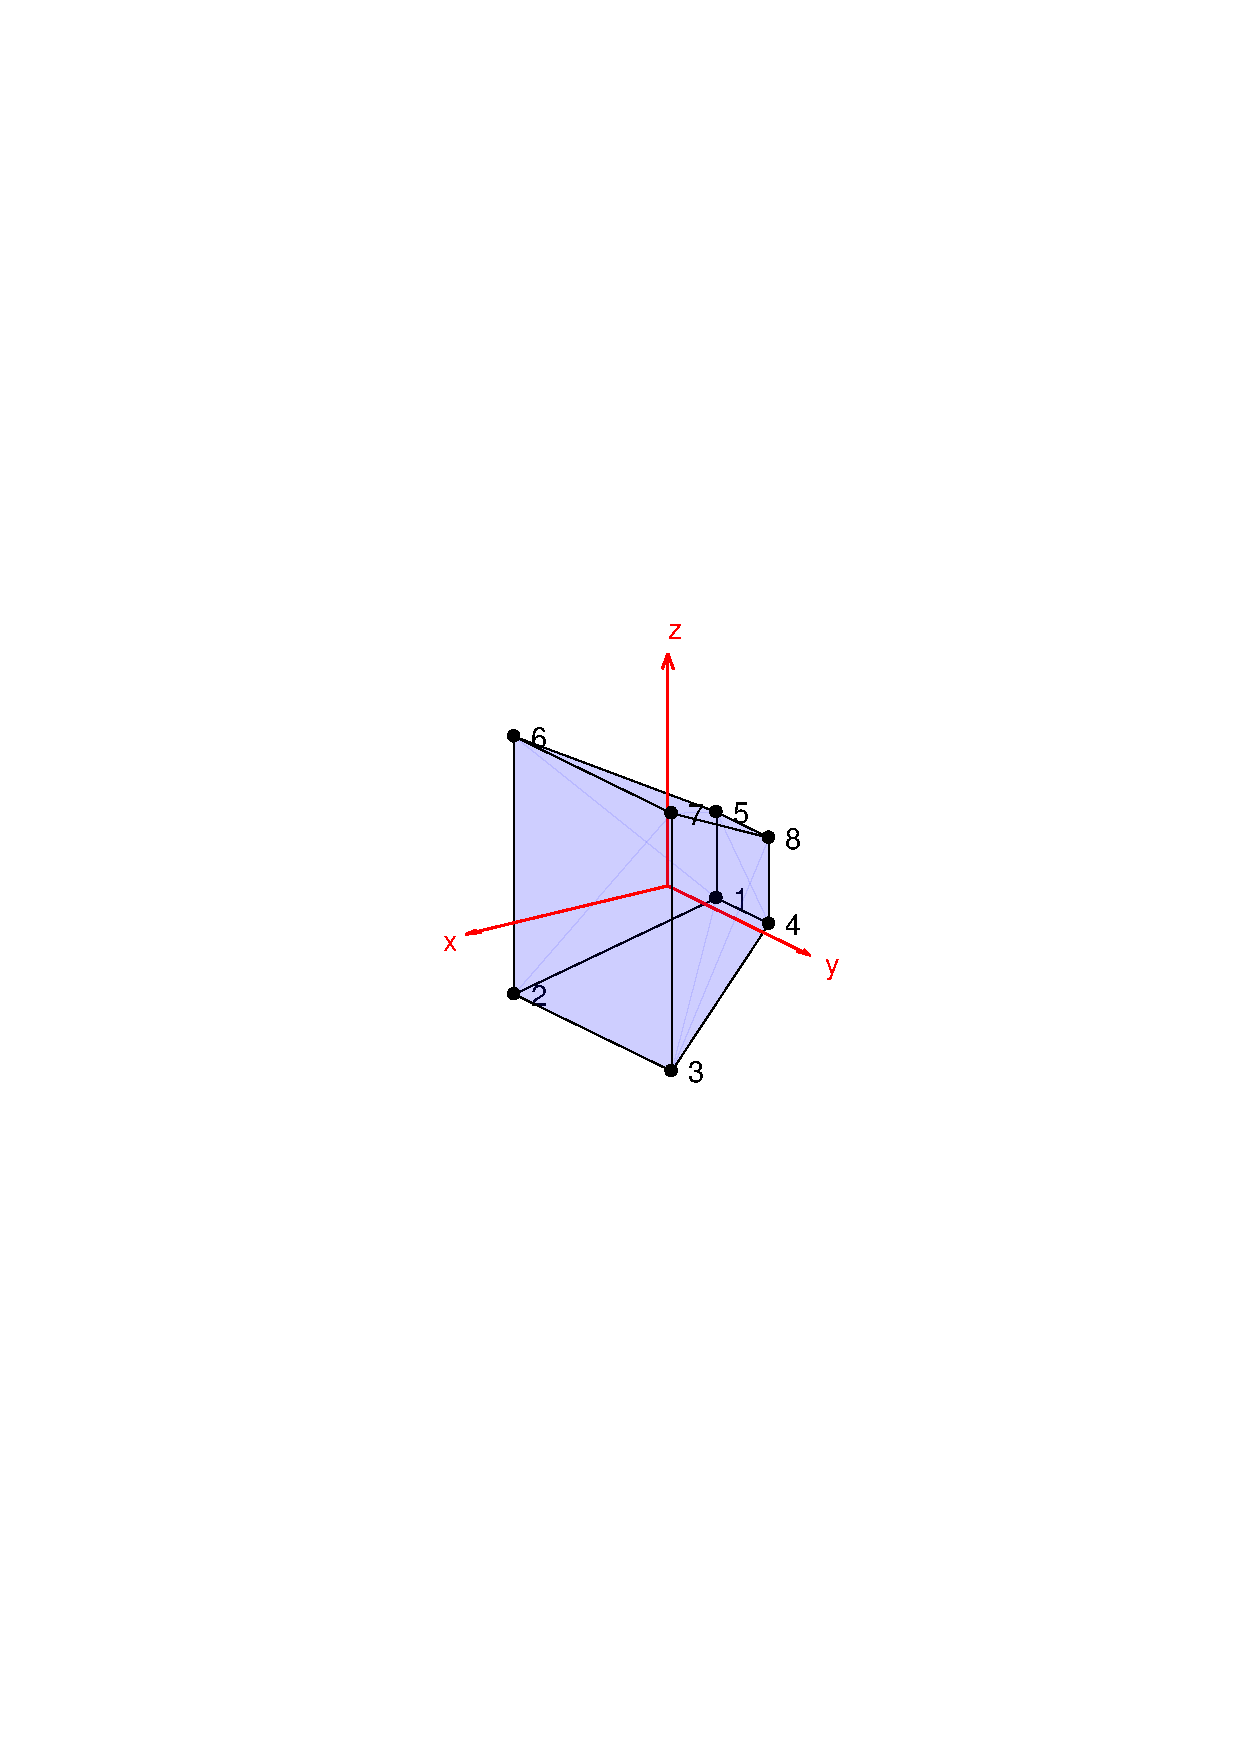
\includegraphics[width=0.5\textwidth]{code_matlab/mapped_element.png}
     }
     \caption{Classic Mapping in FEA}
     \label{fig.1.2}
   \end{figure}
The mapping between reference and actual geometry within a finite element is also made by the same shape functions as follows:
\begin{equation}
\label{eq.1.16}
\VectorVar{X_g}=\VectorVar{\begin{array}{c}
x\\y\\z
\end{array}}=\MatrixVar{\begin{array}{c}\VectorVar{x_n}^T\\\VectorVar{y_n}^T\\\VectorVar{z_n}^T\end{array}}\VectorVar{N_n(\xi,\eta,\zeta)}
\end{equation}
Where  $\VectorVar{x_n},\VectorVar{y_n},\VectorVar{z_n}$ are the column vectors containing the $x,y$ and $z$ coordinates of element nodes, and  $\VectorVar{N_n(\xi,\eta,\zeta)}$ is the column vector containing the value of shape functions relative to element nodes. 
To determine the form of the shape functions one can observe that putting in input the element node reference coordinates $\xi_i,\eta_i,\zeta_i$, for $i=1,2,...,N$, back  into equation \eqref{eq.1.16} one should find the corresponding nodal coordinates $x_i,y_i,z_i$. This means that all shape functions have to satisfy $N$ different interpolation conditions. For this reason, in the case of 8 node hexahedral elements, each shape function is chosen to have the following form:
\begin{equation}
N_i(\xi,\eta,\zeta)=\VectorVar{\begin{array}{cccccccc}
1&\xi&\eta&\zeta&\xi\eta&\xi\zeta&\eta\zeta&\xi\eta\zeta
\end{array}}\VectorVar{\begin{array}{c}
a_{i000}\\a_{i100}\\a_{i010}\\a_{i001}\\a_{i110}\\a_{i101}\\a_{i011}\\a_{i111}
\end{array}}=\VectorVar{p(\xi,\eta,\zeta)}^T\VectorVar{a_i}
\end{equation}
then one can also write:
\begin{equation}
\VectorVar{N_n(\xi,\eta,\zeta)}=\MatrixVar{\begin{array}{c}
\VectorVar{a_1}^T\\
\VectorVar{a_2}^T\\
\vdots\\
\VectorVar{a_8}^T
\end{array}}\VectorVar{p(\xi,\eta,\zeta)}=\MatrixVar{A}\VectorVar{p(\xi,\eta,\zeta)}
\end{equation}
To find the 64 coefficients of $\MatrixVar{A}$ one can employ the 8 interpolation conditions specific to each shape function:
\begin{equation}
\label{eq1.19}
\MatrixVar{\begin{array}{c}\VectorVar{x_n}^T\\\VectorVar{y_n}^T\\\VectorVar{z_n}^T\end{array}}=\MatrixVar{\begin{array}{c}\VectorVar{x_n}^T\\\VectorVar{y_n}^T\\\VectorVar{z_n}^T\end{array}}\MatrixVar{A}\MatrixVar{\begin{array}{cccc}
\VectorVar{p(\xi_1,\eta_1,\zeta_1)}&\VectorVar{p(\xi_2,\eta_2,\zeta_2)}&\cdots&\VectorVar{p(\xi_8,\eta_8,\zeta_8)}
\end{array}}
\end{equation}
Where $\xi_i,\eta_i,\zeta_i$ are nodal reference coordinates and can be obtained as the components of the following vectors:
\begin{eqnarray}
	\VectorVar{\xi}=\VectorVar{\begin{array}{c}
		-1\\1\\1\\-1\\-1\\1\\1\\-1
		\end{array}} \quad \VectorVar{\eta}=\VectorVar{\begin{array}{c}
		-1\\-1\\1\\1\\-1\\-1\\1\\1
		\end{array}} \quad\VectorVar{\zeta}=\VectorVar{\begin{array}{c}
		-1\\-1\\-1\\-1\\1\\1\\1\\1
		\end{array}}
\end{eqnarray}
To satisfy equation \eqref{eq1.19} one must have:
\begin{equation}
\MatrixVar{A}=\MatrixVar{\begin{array}{cccc}
\VectorVar{p(\xi_1,\eta_1,\zeta_1)}&\VectorVar{p(\xi_2,\eta_2,\zeta_2)}&\cdots&\VectorVar{p(\xi_8,\eta_8,\zeta_8)}
\end{array}}^{-1}
\end{equation}
Using the discretization of equation \eqref{eq.1.11}, the problem of equation \eqref{eq.1.10} can be written as the well-known system of equation:
\begin{equation}
\label{eq.1.13}
\MatrixVar{K}^{(h)}\VectorVar{u}^{(h)}=\VectorVar{f}^{(h)}
\end{equation}
Typically $\MatrixVar{K}^{(h)}$ and $\VectorVar{f}^{(h)}$ are called \textit{stiffness matrix} and \textit{load vector}. They are defined as:
\begin{eqnarray}
\label{eq.1.14}
{K}_{i,j}^{(h)}=\int_{\Omega}{\left(\MatrixVar{\nabla_{sym}N_i}^{(h)}\right)^T E\MatrixVar{D}\MatrixVar{\nabla_{sym}N_j}^{(h)}   d\Omega}\\
\label{eq.1.15}
{f}_{i}^{(h)}=\int_{\partial \Omega_{\sigma}}{(\MatrixVar{N_i}^{(h)} \cdot \VectorVar{\bar{t}} )d\partial \Omega}+\int_{\Omega}{(\MatrixVar{N_i}^{(h)}\cdot \VectorVar{b}) d\Omega}
\end{eqnarray}
Here the column vectors $\MatrixVar{N_i}^{(h)}$ and $\MatrixVar{N_j}^{(h)}$ are respectively the i-th and j-th column of $\MatrixVar{N}^{(h)}$.
The integrals of equations \eqref{eq.1.14} and \eqref{eq.1.15} can be decomposed as the sum of the integrals computed on each finite element: 
\begin{eqnarray}
{K}_{i,j}^{(h)}=\sum_{el=1}^{n_{el}}E_{el}\int_{\Omega_{el}}{\left(\MatrixVar{\nabla_{sym}N_i}^{(h)}\right)^T \MatrixVar{D}\MatrixVar{\nabla_{sym}N_j}^{(h)}   d\Omega_{el}}\\
{f}_{i}^{(h)}=\sum_{el=1}^{n_{el}}\int_{\partial \Omega_{\sigma}\cap\partial \Omega_{el} }{(\MatrixVar{N_i}^{(h)} \cdot \VectorVar{\bar{t}} )d\partial \Omega_{el}}+\int_{\Omega_{el}}{(\MatrixVar{N_i}^{(h)}\cdot \VectorVar{b}) d\Omega_{el}}
\end{eqnarray}
Where the Young's modulus was supposed to be uniform over each finite element.
 These integrals are usually evaluated by Gauss quadrature over each element.
The mapping of equation \eqref{eq.1.16} can then be employed:
 \begin{eqnarray}
 {K}_{i,j}^{(h)}=\sum_{el=1}^{n_{el}}E_{el}\sum_{k=1}^{N_{GP}}{\left(\MatrixVar{\nabla_{sym}N_{ik}}^{(h)}\right)^T \MatrixVar{D}\MatrixVar{\nabla_{sym}N_{jk}}^{(h)}\determinant{\MatrixVar{J_k}}\omega_k}\\
 {f}_{i}^{(h)}=\sum_{el=1}^{n_{el}}\sum_{l=1}^{n_{GP}} {(\MatrixVar{N_{il}}^{(h)} \cdot \VectorVar{\bar{t_l}} )\determinant{\MatrixVar{J_l}}\omega_l}+\sum_{k=1}^{N_{GP}}{(\MatrixVar{N_{ik}}^{(h)}\cdot \VectorVar{b_k}) \determinant{\MatrixVar{J_k}}\omega_k}
 \end{eqnarray}
Where the notation $\MatrixVar{\nabla_{sym}N_{ik}}$ means that the i-th column of the matrix containing $\MatrixVar{\nabla_{sym}N_{i}}$ is computed on the k-th Gauss point of the el-th element, $\omega_k$ refers to the integration weights of the Gauss-Legendre integration rule chosen to compute each integral. Moreover due to the variable change, the Jacobian determinant of the geometrical mapping $\determinant{\MatrixVar{J_k}}$ has to be computed in each Gauss point of each element in the FEM.
Jacobian determinant can be computed as:
\begin{equation}
\determinant{\MatrixVar{J}} =\determinant{\MatrixVar{\frac{\partial \VectorVar{X_g}}{\partial \xi},\frac{\partial \VectorVar{X_g}}{\partial \eta},\frac{\partial \VectorVar{X_g}}{\partial \zeta}}}=\determinant{\MatrixVar{\begin{array}{c}\VectorVar{x_n}^T\\\VectorVar{y_n}^T\\\VectorVar{z_n}^T\end{array}} \MatrixVar{A}\MatrixVar{\frac{\partial \VectorVar{p}}{\partial \xi},\frac{\partial \VectorVar{p}}{\partial \eta},\frac{\partial \VectorVar{p}}{\partial \zeta}}} 
\end{equation}
In this expression one can observe that both $\MatrixVar{A}$, and $\MatrixVar{\frac{\partial \VectorVar{p}}{\partial \xi},\frac{\partial \VectorVar{p}}{\partial \eta},\frac{\partial \VectorVar{p}}{\partial \zeta}} $ only depend on the reference element nodal coordinates and on the Gauss point position in the reference space and not on the nodal coordinates of the finite element.
For the expression of $\MatrixVar{\nabla_{sym}N_i}^{(h)}$ one can apply the definition of $\nabla_{sym}$ operator in equation \eqref{eq.1.10} to the i-th column of $\MatrixVar{N}^{(h)}$:
\begin{equation}
	\MatrixVar{\nabla_{sym}N_i}^{(h)}=\VectorVar{\begin{array}{c}
		\frac{\partial N_{1i}}{\partial x}\\\frac{\partial N_{2i}}{\partial y}\\\frac{\partial N_{3i}}{\partial z}\\
		\frac{\partial N_{1i}}{\partial y}+\frac{\partial N_{2i}}{\partial x}\\\frac{\partial N_{1i}}{\partial z}+\frac{\partial N_{3i}}{\partial x}\\\frac{\partial N_{2i}}{\partial z}+\frac{\partial N_{3i}}{\partial y}
		\end{array}}
\end{equation}
Where $N_{1i},N_{2i},N_{3i}$ indicate the first, the second and the third component of the i-th column of  $\MatrixVar{N}^{(h)}$.
Computing $\MatrixVar{\nabla_{sym}N_i}^{(h)}$ is a non-trivial operation since shape functions are expressed in terms of reference variables $(\xi,\eta,\zeta)$, that map through equation \eqref{eq.1.16} the $(x,y,z)$ space. So the inverse mapping between reference and geometric space is an implicit set of functions that often cannot be reversed explicitly. To compute the shape function derivatives with respect to space variable one can use Jacobian matrix definition \footnote{Jacobian matrix of the geometric mapping is nonsingular when finite elements are not twisted and have all distinct nodes}:
\begin{equation}
\MatrixVar{\frac{\partial N_{li}}{\partial x},\frac{\partial N_{li}}{\partial y},\frac{\partial N_{li}}{\partial z}}= 
\MatrixVar{J}^{-1}\VectorVar{\begin{array}{c}
	\frac{\partial N_{li}}{\partial \xi}\\\frac{\partial N_{li}}{\partial \eta}\\\frac{\partial N_{li}}{\partial \zeta}\end{array}} 
\end{equation}
Thanks to these relationships, the system of balance equation can be expressed in terms of a linear system of equations. This system is actually singular, in fact as a last step one needs to apply the boundary conditions (equation \eqref{eq.1.2}). For brevity we will here after refer to stiffness matrix as $\MatrixVar{\mathbf{K_{tot}}}$, to the load vector as $\VectorVar{f_{tot}}$ and to the displacement vector as  $\VectorVar{u}$:
\begin{equation}
\label{eq.1.32}
\MatrixVar{\mathbf{K_{tot}}}\VectorVar{u_{tot}}=\VectorVar{f_{tot}}
\end{equation} The load vector can actually be decomposed in two components: the external load vector $\VectorVar{F}$ coming from applied load and the reaction forces vector $\VectorVar{R}$ coming from the boundary conditions so that:
\begin{equation}
\VectorVar{f_{tot}}=\VectorVar{F}+\VectorVar{R}
\end{equation}
To apply the boundary conditions it is useful to adopt a partition of degrees of freedoms in two sets:
the set of constrained DOFs $\VectorVar{u_b}$ and the set of free DOFs $\VectorVar{u_f}$. According to this partition equation \eqref{eq.1.13} becomes:
\begin{eqnarray}
\label{eq.1.17}
\MatrixVar{\mathbf{K_{bb}}}\VectorVar{u_b}+\MatrixVar{\mathbf{K_{bf}}}\VectorVar{u_f}=\VectorVar{R_b}+\VectorVar{F_b}\\
\label{eq.1.18}
\MatrixVar{\mathbf{K_{fb}}}\VectorVar{u_b}+\MatrixVar{\mathbf{K_{ff}}}\VectorVar{u_f}=\VectorVar{R_f}+\VectorVar{F_f}
\end{eqnarray}
The reaction force is applied only on constrained DOFs so that $\VectorVar{R_f}=\VectorVar{0}$. If all rigid modes are constrained by the boundary conditions, then $\MatrixVar{\mathbf{K_{ff}}}$ is non-singular.
 In this case, the system of equations \eqref{eq.1.17}-\eqref{eq.1.18} can be solved with respect to the unknowns $\VectorVar{u_f},\VectorVar{R_b}$:
\begin{eqnarray}
\label{eq.1.19}
\VectorVar{u_f}=\MatrixVar{\mathbf{K_{ff}}}^{-1}\left(-\MatrixVar{\mathbf{K_{fb}}}\VectorVar{u_b}+\VectorVar{F_f}\right)\\
\label{eq.1.20}
\VectorVar{R_b}=\MatrixVar{\mathbf{K_{bb}}}\VectorVar{u_b}+\MatrixVar{\mathbf{K_{bf}}}\VectorVar{u_f}-\VectorVar{F_b}
\end{eqnarray}
Another way of dealing with boundary conditions that can be more suitable for Multi-Grid solver is replacing the rows relative to constrained DOFs directly with the corresponding kinematic constraint equations.
To keep stiffness matrix symmetry for non-homogeneous Boundary Conditions, the term  $\mathbf{K_{fb}}\VectorVar{u_b}$ has to be considered directly in the right hand side.
\begin{eqnarray}
\label{eq.1.17s}
\MatrixVar{\mathbf{A_{bb}}}\VectorVar{u_b}=\VectorVar{b_b}\\
\label{eq.1.18s}
\MatrixVar{\mathbf{K_{ff}}}\VectorVar{u_f}=\VectorVar{F_f}-\MatrixVar{\mathbf{K_{fb}}}\VectorVar{u_b}
\end{eqnarray}
Note that for simple clamping conditions $\MatrixVar{\mathbf{A_{bb}}}$ is the identity matrix and $\VectorVar{b_b}=0$  so that also $\MatrixVar{\mathbf{K_{fb}}}\VectorVar{u_b}$ is zero.
The advantage of this alternative formulation is that the kinematic constraints are directly included in the global stiffness matrix, making it easier to make the transfer among discretization levels for multigrid solvers, as it will be discussed later in this chapter.
In most of commercial software a post processing can be applied to compute both the deformation field and the stress field on each finite element of the FEM. To do that one needs to apply equation \eqref{eq.1.10} and \eqref{eq.1.11}. As the shape functions are $C^0$ function, their derivatives are actually discontinuous passing from a finite element to the other. Moreover it has been shown that stress and deformations computed through the FEA are the most accurate when computed at the Gauss Points \cite{zlamal1978superconvergence,zhang2006natural}. For this reason in the preprocessing phase, when the stiffness matrix and the load vector are assembled, the following matrixes are commonly stored to be reused in the post processing phase:
\begin{eqnarray}
\label{eq.1.40}
	\VectorVar{\varepsilon}=\MatrixVar{B_{gp}}\VectorVar{u_{el}} \quad
	\VectorVar{\sigma}=\MatrixVar{D}\MatrixVar{B_{gp}}\VectorVar{u_{el}}
\end{eqnarray}
Where $\MatrixVar{B_{gp}}$ is a $6\times 24$ matrix called stiffness-displacement as it links the value of deformations in a given Gauss point with $\VectorVar{u_{el}}$ that indicates the $24\times1$ vector of DOFs for the corresponding element.
\section{A generic engine FEM for fuel consumption variation computation}
As discussed in the introduction, to compute the effect of a given design structure on tip clearance variation control, one needs to consider a mechanical model of the engine, nacelle and pylon (that hereafter we can also describe as Power-Plant System (PPS)). This requires to build the model of each component and then to assemble them together.
In this section we first introduce the engine finite element model employed as demonstrator. Then the post processing steps needed for the computation of a global performance index with respect to tip clearance variation is introduced. This will be described as thrust specific fuel consumption variation due to its link to the actual engine performance deterioration, induced by clearance variation. The reader can also observe that for the reasons discussed in the introduction, this parameter is also correlated to other issues such as engine life and operability.
\subsection{Structural Model}
\label{ssec1.2.1}
The mechanical behavior of both engine and PPS structure is usually studied using a Finite Element Model, integrating complex load combinations. Here we introduce a generic engine model that will be used throughout this work (c.f. figure \ref{enginewem}). 
\begin{figure}[hbt!]
\centering
\includegraphics[width=1\textwidth]{images/Ch1/enginegeometry}
\caption{Proposed Whole Engine Model (WEM). Colors identify zone with different properties. The connection between rotor and stator is represented by rigid connections at bearing locations.\label{enginewem}}
\end{figure}
This model is a simplification of an industrial engine model that in general can have a fan casing structure, a core casing structure and multiple shafts for rotors. The following assumptions are made regarding the model's mechanical behavior. Rotor shafts are modeled using just one beam model. Both fan casing and core casing are represented using shell models. Different properties are employed for each engine module casing. The connection between rotor and stator is made through four rigid connections that represent stator vane and bearing housing in the engine. Outlet guide vanes which connect the core casing to the fan casing are represented with radial beam model tied to each interface of the engine. The thermal and centrifugal expansion of rotor blades are not considered in our analysis and nonlinearities are neglected. Only aerodynamic loads linked with the aircraft maneuvers are considered for simplicity. These loads are applied statically. A general 3D solid design zone is integrated between the wing and the engine (see gray elements in figure \ref{f.1}). This is the zone where the topology optimization will need to find the optimal material placement. For simplicity and since this does not have a significant effect on optimization, we did not consider the air inlet and the nacelle structure.  The engine core casing and the design zone meshes are tied at specific region of compressor and turbine casing. For this reason the solution of the topology optimization problem will be connected to the engine at these same regions. This will avoid solutions connected on prohibited region such as the combustion chamber casing. The techniques employed for the connection between engine casing and design zone mesh will be detailed in section \ref{sec1.3}.
\begin{figure}[hbt!]
\centering
\includegraphics[width=1\textwidth]{images/Ch1/FEM_intro.eps}
\caption{\label{f.1} Engine and design zone (in gray) finite element model. The engine model is made of 9976 finite elements, 9312 linear quadrilateral elements of type and 664 beam elements. The solid design zone is clamped at the orange points representing a clamping to the wing.}
\end{figure}
Eight node brick elements were used to mesh the design zone and full eight points integration was employed for elementary stiffness matrix and stress evaluation. The design zone model is clamped at the wing interface position. The axial load on the engine is applied with concentrated forces on the shaft nodes and with distributed loads on the engine casing. Vertical and lateral loads are distributed uniformly on the circumference of fan stage. % The connection between shaft node and engine casing nodes at bearing positions are modeled using rigid Kinematic couplings i.e. rigid connections. 
The commercial software Abaqus 13.2 was employed for mesh generation and load case application.
\subsection{Performance Model}
\label{ssec1.2.2}
The performance function that we considered in this work is a simplification of the real Thrust Specific Fuel Consumption (TSFC) variation induced by the considered loading conditions. Engine fuel consumption could be impacted in different ways by the pylon and casing design. Here we only considered the effect of closures variations.
The tip clearance variation is described in figure \ref{f.2}, and defined in equation \eqref{eq.1}.
  \\
  \begin{figure}[hbt!]
  \centering
       \subfloat[ \label{f.2a}]{%
         \includegraphics[width=0.4\textwidth]{images/Ch1/tip_def1.eps}
       }
       \subfloat[\label{fig.2b}]{%
         \includegraphics[width=0.4\textwidth]{images/Ch1/tip_def2.eps}
       }
       \caption{Rotor and stator displacements under maneuvers loads: (a) $z-y$ engine section diagram for a given rotor stage. The red structure stands for the rotor, the blue curve for the deformed stator. (b) diagram illustrating radial displacement effect.
       The resulting tip clearance is the sum of the initial clearance $\delta_0$ and its variation induced by the engine deformation $\delta(\theta)$ }
       \label{f.2}
     \end{figure}
  \\
\begin{equation}
\label{eq.1}
\delta(\theta)=u_r^c(\theta)-u_r^b(\theta)=\lbrace r( \theta ) \rbrace^T \cdot \left( \lbrace u^c(\theta) \rbrace-\lbrace u^b(\theta) \rbrace\right)
\end{equation}
Where $u_r^c(\theta)$ and $u_r^b(\theta)$  are the radial displacements of casing and rotor blade tip respectively at the angular position $\theta$ and $\lbrace r( \theta ) \rbrace$ is the radial unit vector at the angle $\theta$ .
Considering an angular discretization of the circumference given by the stator mesh in the $s^{th}$ engine stage, $\theta^i_{(s)}$ the tip clearance variation at the angular section $i$ is then:	
\begin{equation}
\lbrace\delta_{(s)}\rbrace_i=\lbrace r( \theta^i_{(s) } \rbrace^T \cdot \left( \lbrace u^c(\theta^i_{(s)} \rbrace-\lbrace u^b(\theta^i_{(s)} \rbrace\right)
\end{equation}
That is actually a system of linear relationships that can be expressed in the matrix form:
\begin{equation}
\label{e.3}
\lbrace\delta_{(s)}\rbrace =\left[ \gamma_{(s)} \right] \lbrace U \rbrace
\end{equation}
where $\lbrace U \rbrace$ is the displacements vector.
To characterize a stage's contribution to the overall engine performance, tip-clearance's variation Root Mean Square (RMS) is evaluated at each stage:
\begin{equation}
\label{e.4}
R_{(s)} =\sqrt{\frac{\lbrace\delta_{(s)}\rbrace^T\lbrace\delta_{(s)}\rbrace}{N_{(s)}}}
\end{equation}
where $N_{(s)}$ is the number of nodes used for the angular discretization of the $s^{th}$ stage. 
In this thesis, we use a simple model to link the tip clearances to the TSFC performance. The variation in TSFC due to aircraft maneuvers is considered here as a linear combination of the RMS values per stage:
\begin{equation}
\label{e.5}
\Delta TSFC \% = \sum_{s=1}^{ns}\frac{R_{s}}{l_{(s)}}100
\end{equation}
where $ns$ is the number of stages of the engine and $l_{(s)}$ the stage blade height.
When considering several maneuvers, in order to get a single value of performance one can adopt several approaches.
In an industrial modeling attempt, the TSFC variation relative to a given load case needs to be weighted using the probability of occurrence  of the corresponding flight condition in the product life. 
In this attempt one should consider:
\begin{equation}
\label{e.5b}
\Delta TSFC \% = \sum_{lc=1}^{N_l}f_{lc}(\Delta TSFC \%)_{lc}
\end{equation}
Where $N_l$ is the number of flight points considered, $(\Delta TSFC \%)_{lc}$ and $f_{lc}$ is the corresponding TSFC variation and the probability of occurrence respectively. To give an insight on this formula, one can observe that for each aircraft family one will have different weighting for each loading condition. In reality one can observe that this model does not reflect the actual design process of an actual engine, neither the correlation between several operating conditions. A turbofan engine initial clearance $\delta_0$ should in fact be designed to avoid casing to blade contact in any operating conditions. This means that:
\begin{equation}
(\delta_0)_s=\max{\left(0, \min_{l}{\left((\delta_{(s)})_l\right)}\right)}
\end{equation}
By the use of equation \ref{e.5b}, this time one can observe that the effect of load cases generating larger negative tip clearance variations, will also affect the performance in situations where the tip clearance variations are smaller. This means that load cases having larger negative variations will be the one that affect the most the specific fuel consumption variation. Due to that observation when considering several loading conditions a good indicator of the final performance can be associated to the highest TSFC variation (which is considered to be also linked to load cases that generate the largest negative tip clearance variations):
 \begin{equation}
 \label{e.5c}
 \Delta TSFC \% = \max_l(\Delta TSFC \%)_l
 \end{equation}
\section{Tying inconsistent meshes}
\label{sec1.3}
An important issue that needs to be addressed is the mesh inconsistency between engine and design zone. In fact the Engine Finite Element Model in the current practice is built by the engine manufacturer and is not initially intended for use in a topology optimization framework. For this reason in order to freely mesh the design zone we would like to be able to put these two non-overlapping domains in connection trough their interface DOFs.\\
 The first hypothesis made is that only translational DOFs of engine shell elements have to be considered for kinematic tying. For this reason the engine condensation (c.f. subsection \ref{subsection1.4.1}) was performed around the retained nodes translational DOFs and not for rotational DOFs, that are therefore not constrained. The external skin of the engine's shell elements need to have the same displacements as the external surface of the solid elements. Many techniques can be employed for dealing with this problem as described in the review \cite{coniglio2018weighted}. Situations arise where a finite element model needs to be assembled from parts that can present non-matching grids (meshes). In these cases the displacement at the interface is not uniquely determined and special techniques have to be used to take into account the non-conforming interface \cite{mcgee2005non}. \\
 This can be the case:
 \begin{itemize}
     \item When two parts have to be meshed independently for practical reasons \cite{barlow1982constraint,quiroz1995non}. This can be due to the impossibility to get good quality meshes for two adjacent components or due to models being generated independently by different teams or for different purposes, or even for modularity if one component model has to be integrated in different product models. 
     \item When different physical phenomena are studied with different discretizations: for example in acoustics \cite{flemisch2012non}. One of the most popular applications is Fluid-Structure Interaction (FSI) \cite{de2007review,de2008comparison,hou2012numerical,beckert2001multivariate,cebrali1997conservative,lohner1998fluid,farhat1998load}. The mesh needed for the fluid is much finer than the one that needs to be used for solid. Important computation time can be saved using mesh projection techniques to connect different meshes.
     \item When the domain decomposition is required (\cite{brandt2002multiscale,feyel2000fe,duval2016non,farhat1991method,mandel1993balancing}. The communication between the large scale and lower scale meshes is often done with a mesh projection operator. Such domain decomposition is for example useful when a much finer mesh is needed in a localized region of a structure (e.g. in crack propagation analysis \cite{duval2016non,lloberas2012micro,lloberas2012multiscale}).
     \item When contact between meshes is activated in the simulation \cite{wriggers1995finite,shillor20047,sofonea2005analysis,christensen1998formulation}. In the most general situation rebounding and sliding can appear the exchange of information between meshes changes  with the grid configurations. In this application the mesh projection operator has to be computed fast enough so that its evaluation can be repeated in the analysis.
 \end{itemize}
 \subsection{State of the art}
 The main challenge of the aforementioned situation is to ensure the continuity of the displacement field at the non-conforming interface. In the general case of non-matching interfaces, the displacement field will be continuous at the cost of an over-constraint of the interface \cite{rixen1997substructuring}. To avoid this phenomenon, typically both strong and weak coupling can be employed to satisfy the compatibility of the solution at the interface node DOFs.
 \subsubsection{Strong and weak formulations}
  The strong coupling techniques are also referred to as collocation techniques \cite{rixen1997substructuring,aminpour1995coupled} or node to segment \cite{wriggers1995finite}, as one constraint equation is assigned to each interface node DOF. In the weak coupling, also called segment to segment \cite{wriggers1995finite} methods, on the other hand, the continuity is written in an integral or averaged sense. To avoid interface stiffening, the weak formulation is preferred \cite{aminpour1995coupled,fish1995iterative}. 
 For both these "classic" approaches, one surface is chosen to be the one that will produce the constraint equations (slave surface) and the other is considered as interpolating (master surface). Each DOF of the slave surface is then written as a linear combination of the DOFs of the master surface. Once that this linear system of constraint equations is written, the final displacement solution can be obtained by the elimination method \cite{barlow1982constraint} i.e. substituting the slave node DOFs variable with their expression in terms of master node DOFs. Since the solution of a static solid analysis can also be considered as a minimization problem, the linear constraints can be imposed using the Lagrange multipliers approach \cite{bertsekas2014constrained,babuvska1973finite}.  A variable is therefore created for each constraint that has to be satisfied and used to build the Lagrangian function.  The stationarity conditions of the Lagrangian function give the linear system of equations used to find the nodal displacement and the interface Lagrange multiplier variables. The latter also have the physical interpretation of interface internal forces.
 One of the most used techniques that utilizes Lagrange multipliers in a continuous form is the Mortar approach \cite{bernardi1993domain,bernardi1989new,puso20043d,puso2004mortar}.The distribution functions for the Lagrange multipliers and shape functions for
 the finite elements should be properly selected to fulfill the Ladyzhenskaya-Babu\v{s}ka-Brezzi (LBB) condition (also known as the inf-sup condition) \cite{babuvska1997babuvska} in order to guarantee that both discretizations converge to the correct solution with the mesh refinement.
\subsubsection{Alternative and improved approaches}
 Other numerical schemes followed, inspired by the optimization community. In the PhD dissertation of Rixen \cite{rixen1997substructuring} one can find a method based on the augmented Lagrangian method in optimization. In the review of  Barlow \cite{barlow1982constraint} another method based on the external penalty approach is presented. 
 The main difficulty of this approach consists in the choice of the penalty factor. 
 Deparis et al. introduced in \cite{deparis2016internodes} a new approach based on the simultaneous continuity of the displacement and the internal loads per unit of area at the interface. This promising technique has been tested in the case of a simple patch test and more complex fluid structure interaction problems. In those cases the method reveals the same performance as Mortar, with a much smaller computational effort and programming complexity. 
 In order to pass \textit{\textit{\textit{a priori}}} the simple stress patch test even for curved interfaces where Mortar typically fails,  Park et al \cite{park2002simpl} developed a method  based on the introduction of a third displacement field whose nodes are placed based on an equilibrium equation of moments. The resulting scheme is however quite complex and the applications considered in \cite{park2002simpl} where only for a simple 2D case and a planar interface on a 3D case. 
 For overlapped domains with non-consistent meshes the Arlerquin method has also been proposed \cite{dhia2005arlequin,dhia2008multimodeling}.
 More invasive approaches were developed by Cho et al. \cite{cho2005improved,cho2006mls,cho2006mlsII},Lim et al. \cite{lim2007mls,lim2007variable} , Kim et al. \cite{kim2003interface} and Duarte \cite{duarte2008analysis}, where the idea is to modify the Element shape functions adding some nodes to the element of the interface or enriching the shape functions. In Dohrman et al. \cite{dohrmann2000method,dohrmann2000methods} the slave element locations and formulations are modified in order to transform a non-conforming interface into a conforming one.
 In Tian et al. \cite{tian2007non} interface elements formulation is replaced with a meshless formulation. 
 In this way the coupled analysis becomes straightforward  but the implementation of a special formulation for interface elements is not as simple as the application of multi-point constraints (MPCs) at the interface. 
 A Least Square Method can be found in Bochev et al. \cite{bochev2007least} in order to pass a simple patch test. This method requires nevertheless the meshes to be perturbed at the interface to avoid gaps between curved interfaces, which render the approach more complex to implement.
 Bitencourt et al. \cite{bitencourt2015coupling} introduced a new method that assembles Coupling Finite Elements (CFEs) at the interface to build the constraints equation between interfaces Degrees of Freedom (DOFs). This approach was studied for 3D planar, 2D planar or 2D curved interfaces. 
 A recent method was developed by Cafiero et al. \cite{cafiero2016domain} on the base of the previous developments of Nitsche  \cite{nitsche1971variationsprinzip}, Becker \cite{becker2003finite}, Heintz \cite{heintz2006stabilized} , Olivier \cite{oliver2009contact} and Hartman \cite{hartmann2009contact}. This approach, inspired from the contact community avoids the expensive segment to segment projections needed for the mortar approach introducing a particular formulation in the gap between the non-conforming meshes at the interface. The Domain Interface Method (DIM) \cite{cafiero2016domain} was also extended to the case of mixed fields as can be encountered in multiphysics problems \cite{lloberas2017domain}. Another similar approach introduced virtual gap elements at the interface of the domains and imposes a zero strain condition to these elements \cite{song2017virtual}.
 \\
 \subsection{Domain partition}\label{ssec22}
 We consider here the same problem but this time we consider a partition of the domain $\Omega$ into two subdomains $\Omega_1$ and $\Omega_2$ (cf. figure \ref{fig.1.5}). The general case with m subdomain can be easily derived from this case. The surface used for the partition is unique  ($\Gamma_1 \equiv \Gamma_2 \equiv \Gamma$), as a consequence:
 \begin{eqnarray}
 \label{eq.13}
 \VectorVar{u}_{\Gamma_1}=\VectorVar{u}_{\Gamma_2} & \forall \VectorVar{x} \in \Gamma\\
 \label{eq.14}
 \MatrixVar{\sigma}_{\Gamma_1}\cdot\VectorVar{\hat{n}}_{\Gamma_1}=\VectorVar{t}_{12}=-\VectorVar{t}_{21}=-\MatrixVar{\sigma}_{\Gamma_2}\cdot\VectorVar{\hat{n}}_{\Gamma_2} & \forall \VectorVar{x} \in \Gamma
 \end{eqnarray}
 
 \begin{figure}[ht]
 \centering
 \includegraphics[width=8cm]{images/Ch1/free_body}
 \caption{Partition of $\Omega$ in two subdomains $\Omega_1$, $\Omega_2$} 
 \label{fig.1.5}
 \end{figure}
 
 Moreover taking in account the partition we will have:\footnote{In these expression the terms $\int_{\Gamma_1}{(\VectorVar{v} \cdot \VectorVar{t}_{21} )d\Gamma_1}$ and $\int_{\Gamma_2}{(\VectorVar{v} \cdot \VectorVar{t}_{12} )d\Gamma_2}$ are due to the work of internal forces at the boundary. In a variational approach it would naturally vanish considering the work over the whole structure.}
 \begin{equation}
 \begin{aligned}
 \label{eq.15}
 \int_{\Gamma_1}{(\VectorVar{v} \cdot \VectorVar{t}_{21} )d\Gamma_1}+\int_{\partial \Omega_{\sigma_1}}{(\VectorVar{v} \cdot \VectorVar{\bar{t}} )d\partial \Omega}+\int_{\Omega_1}{(\VectorVar{v} \cdot \VectorVar{b}) d\Omega} =\\\int_{\Omega_1}{(\VectorVar{\MatrixVar{D}} \VectorVar{v} :\MatrixVar{\MatrixVar{E}}:\VectorVar{\MatrixVar{D}} \VectorVar{u}  )d\Omega}
 \end{aligned}
 \end{equation}
 \begin{equation}
 \begin{split}
 \label{eq.16}
 \int_{\Gamma_2}{(\VectorVar{v} \cdot \VectorVar{t}_{12} )d\Gamma_2}+\int_{\partial \Omega_{\sigma_2}}{(\VectorVar{v} \cdot \VectorVar{\bar{t}} )d\partial \Omega}+\int_{ \Omega_2}{(\VectorVar{v} \cdot \VectorVar{b}) d\Omega}=\\\int_{ \Omega_2}{(\VectorVar{\MatrixVar{D}} \VectorVar{v} :\MatrixVar{\MatrixVar{E}}:\VectorVar{\MatrixVar{D}} \VectorVar{u}  )d\Omega}
 \end{split}
 \end{equation}
 That may be combined with equation \eqref{eq.14} to get equation \eqref{eq.1.11b}.
 As expected the virtual partition into subdomain is a choice that does not affect the solution of the elastostatics problem.   
 \\
 \subsection{Domain decomposition with consistent discretization}\label{ssec31}
 When a finite element discretization is used to solve the elastostatic problems over the subdomains $\Omega_1$ and $\Omega_2$, the interface will be discretized in the surfaces $\Gamma_1^h$ and $\Gamma_2^h$.  
 We call consistent discretization the case where the nodes of the interface are on the same positions for both subdomains $\Omega_1$ and $\Omega_2$ and the shape functions of each element on both sides of the interfaces are the same.
 \begin{figure}[ht]
 \centering
 \includegraphics[width=8cm]{images/Ch1/Consistent_discretization}
 \caption{Consistent discretization of the partitioned domain} 
 \label{fig.3}
 \end{figure}
 \\
 In this case the domain decomposition is not a concrete issue. In fact the communication between the degrees of freedom (DOFs) of the two discretizations is straightforward. We can nevertheless introduce a partition of the DOFs that will be used for each of the latter approaches discussed in this work.
 We will call $\VectorVar{u}_1^{(h)},\VectorVar{u}_2^{(h)},\VectorVar{u}_{\Gamma_1}^{(h)},\VectorVar{u}_{\Gamma_2}^{(h)}$ respectively the DOFs of nodes inside $\Omega_1$ but not on the interface $\Gamma_1$, the DOFs of nodes inside $\Omega_2$ but not on the interface $\Gamma_2$, the DOFs of the nodes of the interface $\Gamma_1$ and the DOFs of the nodes on the interface $\Gamma_2$ respectively. The discretized form of equations \eqref{eq.15}-\eqref{eq.16} is then: 
 \begin{equation}
 \label{eq.23}
     \left[ \begin{array}{cccc} 
     \MatrixVar{\mathbf{K}}_{1,1} & \MatrixVar{\mathbf{K}}_{1,\Gamma_1} & \MatrixVar{0}& \MatrixVar{0} \\
    \MatrixVar{\mathbf{K}}_{\Gamma_1,1} & \MatrixVar{\mathbf{K}}_{\Gamma_1,\Gamma_1} & \MatrixVar{0}& \MatrixVar{0}\\ \MatrixVar{0}& \MatrixVar{0}& \MatrixVar{\mathbf{K}}_{\Gamma_2,\Gamma_2}&\MatrixVar{\mathbf{K}}_{\Gamma_2,2}\\   
     \MatrixVar{0} & \MatrixVar{0}& \MatrixVar{\mathbf{K}}_{2,\Gamma_2} & \MatrixVar{\mathbf{K}}_{2,2}\end{array} \right] \left\lbrace \begin{array}{c} \VectorVar{u}_1\\\VectorVar{u}_{\Gamma_1}\\\VectorVar{u}_{\Gamma_2}\\\VectorVar{u}_2
     \end{array}\right\rbrace= \left\lbrace\begin{array}{c} \VectorVar{f}_1\\\VectorVar{f}_{\Gamma_1}+\VectorVar{r}_{\Gamma_1}\\\VectorVar{f}_{\Gamma_2}+\VectorVar{r}_{\Gamma_2}\\\VectorVar{f}_2
     \end{array}\right\rbrace
 \end{equation}
 The residuals $\VectorVar{r}_{\Gamma_1}$ and $\VectorVar{r}_{\Gamma_2}$ are the expression of the internal forces acting on the interface DOFs of each surface. Equations \eqref{eq.13} and \eqref{eq.14} are easily interpreted in this case, since the node in the same position belonging to both meshes will merge and have the same DOFs.
 This can be expressed as:
 \begin{eqnarray}
 \label{eq.24}
 \VectorVar{u}_{\Gamma_2}=\VectorVar{u}_{\Gamma_1} =\VectorVar{u}_{\Gamma} \qquad
 \label{eq.25}
 \VectorVar{r}_{\Gamma_2}=-\VectorVar{r}_{\Gamma_1}
 \end{eqnarray}
 where it is assumed that the interface DOFs have been sorted giving the same index to corresponding DOFs of corresponding nodes. Substituting equations \eqref{eq.24} back into equation \eqref{eq.23} and eliminating the residuals one can get:
 \begin{equation}
 \label{eq.26}
     \left[ \begin{array}{ccc} 
     \MatrixVar{\mathbf{K}}_{1,1} & \MatrixVar{\mathbf{K}}_{1,\Gamma_1} & \MatrixVar{0} \\
    \MatrixVar{\mathbf{K}}_{\Gamma_1,1} & \MatrixVar{\mathbf{K}}_{\Gamma_1,\Gamma_1}+ \MatrixVar{\mathbf{K}}_{\Gamma_2,\Gamma_2} & \MatrixVar{\mathbf{K}}_{\Gamma_2,2}\\   
     \MatrixVar{0} & \MatrixVar{\mathbf{K}}_{2,\Gamma_2} & \MatrixVar{\mathbf{K}}_{2,2}\end{array} \right] \left\lbrace \begin{array}{c} \VectorVar{u}_1\\\VectorVar{u}_{\Gamma}\\\VectorVar{u}_2
     \end{array}\right\rbrace= \left\lbrace\begin{array}{c} \VectorVar{f}_1\\\VectorVar{f}_{\Gamma_1}+\VectorVar{f}_{\Gamma_2}\\\VectorVar{f}_2
     \end{array}\right\rbrace
 \end{equation}
 Obviously, in the case of a conforming interface equation \eqref{eq.26} could also be obtained using the conforming discretization of equation \eqref{eq.1.11b}. Indeed equations \eqref{eq.1.32} and \eqref{eq.26} are equivalent.
 \subsection{Domain decomposition with non-consistent discretization}\label{ssec32}
 Cafiero et al.  \cite{cafiero2016domain} shows different cases in which the non-conforming discretization can increase the challenge associated with a "transfer" of displacement field and stress tensor between meshes.
 In the following section the different scenarios are reviewed.
 
 \subsubsection{Non conformity scenarios}\label{sssec321}
 The first case we want to address is the simplest one (cf. figure \ref{fig.4}). The interface boundary and area are the same, $\Gamma_1^{h} \equiv \Gamma_2^{h} $, the normal vectors are opposite in each corresponding point of the interfaces. It may be the case, in the context of domain decomposition for a multi-grid approach. The nodes are not in the same position but the shape functions of both domains are still the same. As a consequence, the local balance of the surface traction using a mortar-type approach will also imply the satisfaction of a patch test \cite{park2002simpl}.
 \\
 \begin{figure}[ht]
 \centering
 \includegraphics[width=8cm]{images/Ch1/Mesh_inconsist_1}
 \caption{Inconsistent mesh partition that does not introduce geometric inconsistency: $\Gamma_1^{h} \equiv \Gamma_2^{h} $}  
 \label{fig.4}
 \end{figure}
 
 The second case is the first case of geometric inconsistency due to the non-coincidence of the boundary of the interface (figure \ref{fig.5}).
 \begin{figure}[ht]
 \centering
 \includegraphics[width=8cm]{images/Ch1/Mesh_inconsist_2}
 \caption{Inconsistent mesh partition that introduces geometric inconsistency: $\Gamma_1^{h} \not\equiv  \Gamma_2^{h} $, first case different mesh boundaries} 
 \label{fig.5}
 \end{figure}
  \\
 Still the surface normal is the opposite that means that the patch test may be satisfied by the use of a mortar approach. In figure \ref{fig.6} we present a second case that also produces a geometric inconsistency: when a curved interface is discretized with non-matching meshes, the normal vectors are distinct on each element surface and may not be opposite for corresponding elements\footnote{In this case even the definition of corresponding elements is not straightforward. A possible definition  is that two elements are corresponding if the area of the intersection between one element surface and the projection of the other element surface on the first one is non-zero and if the element center distance is less than a given tolerance }. The area is different on both mesh surfaces. Moreover there can be a gap or intersections of interface mesh surfaces. 
 \begin{figure}[ht]
 \centering
 \includegraphics[width=8cm]{images/Ch1/Mesh_inconsist_3}
 \caption{Inconsistent mesh partition that generates geometric inconsistency: $\Gamma_1^{h} \not\equiv  \Gamma_2^{h} $, second case curbed interface} 
 \label{fig.6}
 \end{figure}
 \\
 In this case the satisfaction of the patch test is only approximated with the use of a mortar approach \cite{park2002simpl}. Another important scenario is the one in figure \ref{fig.7} that shows two domains with the same node position but with different shape functions. 
 \begin{figure}[ht]
 \centering
 \includegraphics[width=8cm]{images/Ch1/Mesh_inconsist_4}
 \caption{Inconsistent mesh partition that introduces geometric inconsistency: $\Gamma_1^{h} \not\equiv  \Gamma_2^{h} $, third case different shape functions} 
 \label{fig.7}
 \end{figure}
 Also in this case the normal and the geometry of the interpolated interfaces are not  coincident, and special methods are needed to deal with this case \cite{wang2017variationally}.The most general scenario could be the combination of one or more of these scenarios, as it will be discussed later.
 
  \subsection{Elimination methods - Master/Slave  approaches}\label{ssec33}
  This is a family of approaches that we can find described in Barlow et al. \cite{barlow1982constraint} and in the review paper of De Boer et al \cite{de2007review} that we briefly summarize and enrich in this section. The main idea consists in the reformulation of equations \eqref{eq.13} and \eqref{eq.14} as linear relationships between the interfaces of the sub-domains. Then, one of the surfaces is chosen as slave ($\Gamma_2$), its DOFs will be explicitly given as function of the DOFs of the master surface ($\Gamma_1$).  
  \begin{equation}
  \label{eq.28}
  \VectorVar{u}_{\Gamma_2}=\MatrixVar{\Pi}_{21}\VectorVar{u}_{\Gamma_1}
  \end{equation}
  From a physical point of view the total work as the resultant force  of the internal forces on the interface should be zero (energy conservation and static balance).
  \begin{eqnarray}
  \label{eq.29}
  \VectorVar{r}_{\Gamma_1}^T\VectorVar{u}_{\Gamma_1}+\VectorVar{r}_{\Gamma_2}^T\VectorVar{u}_{\Gamma_2}=0\\
  \label{eq.30}
  \MatrixVar{1}_{\Gamma_1}^T\VectorVar{r}_{\Gamma_1}+\MatrixVar{1}_{\Gamma_2}^T\VectorVar{r}_{\Gamma_2}=\VectorVar{0}
  \end{eqnarray}
  In which $\MatrixVar{1}_{\Gamma_1}$ and $\MatrixVar{1}_{\Gamma_2}$ are matrices with the number of lines equal to the number of DOFs of interface ${\Gamma_1}$ and ${\Gamma_2}$ and 3 columns (one per each component). For 3D solid elements they are Boolean matrices that have 1 on the component whose line corresponds to the direction given by the index of their column and 0 otherwise. 
   Equations \eqref{eq.29} and \eqref{eq.30} combined with equation \eqref{eq.28} give:
  \begin{eqnarray}
  \label{eq.31}
  \VectorVar{r}_{\Gamma_1}=-\MatrixVar{\Pi}_{21}^T\VectorVar{r}_{\Gamma_2}\\
  \label{eq32}
  \MatrixVar{\Pi}_{21}\MatrixVar{1}_{\Gamma_1}=\MatrixVar{1}_{\Gamma_2}
  \end{eqnarray}
  Equation \eqref{eq32} is a necessary condition that must be satisfied by the projection operator $\MatrixVar{\Pi}_{21}$ defined in equation \eqref{eq.28}. On the other hand, equation \eqref{eq.31} is used with equations \eqref{eq.23} and \eqref{eq.24} to finally get the reduced system of equations:
  \begin{equation}
  \label{eq.33}
  \begin{aligned}
  \left[ \begin{array}{ccc} 
      \MatrixVar{\mathbf{K}}_{1,1} & \MatrixVar{\mathbf{K}}_{1,\Gamma_1} & \MatrixVar{0} \\
     \MatrixVar{\mathbf{K}}_{\Gamma_1,1} & \MatrixVar{\mathbf{K}}_{\Gamma_1,\Gamma_1}+ \MatrixVar{\Pi}_{21}^T\MatrixVar{\mathbf{K}}_{\Gamma_2,\Gamma_2}\MatrixVar{\Pi}_{21} & \MatrixVar{\Pi}_{21}^T\MatrixVar{\mathbf{K}}_{\Gamma_2,2}\\   
      \MatrixVar{0} & \MatrixVar{\mathbf{K}}_{2,\Gamma_2}\MatrixVar{\Pi}_{21} & \MatrixVar{\mathbf{K}}_{2,2}\end{array} \right] \left\lbrace \begin{array}{c} \VectorVar{u}_1\\\VectorVar{u}_{\Gamma_1}\\\VectorVar{u}_2
      \end{array}\right\rbrace= \left\lbrace\begin{array}{c} \VectorVar{f}_1\\\VectorVar{f}_{\Gamma_1}+\MatrixVar{\Pi}_{21}^T\VectorVar{f}_{\Gamma_2}\\\VectorVar{f}_2
      \end{array}\right\rbrace
  \end{aligned}
  \end{equation}
  This is a linear system of equations with a positive semi-definite symmetric matrix like the stiffness matrix of equation \eqref{eq.1.32}. 
  The projection operator $\MatrixVar{\Pi}_{21}$ can be defined using two different approaches that in the contact community are known as node to segment and segment to segment approaches. In the former the relation between the DOFs is given directly by a geometric interpolation. De Boer et al. \cite{de2007review} show two examples of these methods: the Nearest neighbor interpolation (NN) \cite{thevenaz2000interpolation} and the Radial Basis Functions (RBF) \cite{beckert2001multivariate}, \cite{smith2000evaluation}. Another option consists in using of the trace of element shape function on the interface to interpolate the displacement field. In this work we will refer to these methods as Element Shape Function interpolation (ESF).
  The main drawback of these methods is their strong dependence on the slave and master surface choice. In fact for domains meshed with different mesh sizes, choosing the most refined mesh as master surface will not ensure the continuity of the displacement field for all the master nodes that do not belong to elements that contain a slave node projection. Moreover these methods don't satisfy simple patch tests even if the interface is not curved, and finally as it was shown by Bernardi et al. \cite{bernardi1989new} they are sub-optimal in term of mesh convergence.
  The segment to segment approaches even if much more complex to set up can show better accuracy. Finally we present another elimination method based on a weak form of the continuity equation: the Weighted Residual Methods (WRM).
  \begin{comment}
   The most popular approach in the literature in order to solve this problem is the Mortar method  \cite{bernardi1993domain,bernardi1989new,puso20043d,puso2004mortar}, which is well known to have very good performance in terms of displacement optimality convergence, however its implementation is often quite complex. Displacement continuity has been imposed in this work considering the Radial Basis function interpolation  approach proposed by the Deparis et al. in \cite{deparis2014rescaled} based on a B\&W compactly supported radial basis function . This simple collocation approach makes the hypothesis that the displacement field of one discretized surface (commonly called master surface) can be used to evaluate, by interpolation, the displacement field of the other (so called slave surface). Writing kinematic continuity in this way one can have a set of linear relationships between meshes in the form of:
    \begin{eqnarray}
    \lbrace u_c \rbrace = \left[ \Pi_{cd} \right] \lbrace u_{d}\rbrace & ,&\lbrace u_{d} \rbrace = \left[ \Pi_{dc} \right]\lbrace u_{c}\rbrace
    \end{eqnarray}
    Where $\lbrace u_c \rbrace$, $\lbrace u_{d}\rbrace $ are respectively engine and design zone interface DOFs.
    These relationships are used to eliminate slave DOFs from the problem since they can be evaluated by interpolation from master DOFs. The choice of master and slave surfaces in structural finite element analysis is crucial. Commonly, in order to have better stress and displacement accuracy the surface discretized with the finest mesh should be considered as slave and the other as master. In our problem engine retained interface was considered as master and design zone interface as slave. The final set of balance equations for the assembled system is obtained imposing residual and energy balance at the interface. For instance, after eliminating engine DOFs, the final system of equation reads :
    \begin{equation}
    \label{eq.32}
    \left[ \begin{array}{cc}
    \left[ \mathbf{K_{oo}} \right] & \left[ \mathbf{K_{od}} \right]\\
    \left[ \mathbf{K_{do}} \right] & \left[ \mathbf{K_{dd}} \right]+\left[ \Pi_{cd} \right]^T\left[ \mathbf{\tilde{K}_{cc}} \right]\left[ \Pi_{cd} \right]
    \end{array} \right] \left\lbrace \begin{array}{c}
    \lbrace u_o \rbrace\\
    \lbrace u_d \rbrace\\
    \end{array}\right\rbrace =  \left\lbrace \begin{array}{c}
    \lbrace F_o \rbrace\\
    \lbrace F_d\rbrace+\left[ \Pi_{cd} \right]^T\lbrace \tilde{F}_c\rbrace\\
    \end{array}\right\rbrace
    \end{equation} 
    Where $o$ is the index of design zone DOFs not lying on the interface.
    Using these techniques the engine retained nodes stiffness matrix and load vector can be integrated to the design zone. Note that in equation \eqref{eq.32} the only engine interface DOFs are considered (c). Subsection \ref{subsection1.4.1} explains the meaning of this choice and of $\left[ \mathbf{\tilde{K}_{cc}} \right]$ and $\lbrace \tilde{F}_c\rbrace$.
     \end{comment}
     \subsubsection{Radial Basis Function interpolation (RBF)}\label{sssec332}
     For more general applications, the RBF represent a practical and easy to implement solution. In this approach the displacement field at the interface  is supposed to be a linear combination of radial basis functions defined per each node of the master surface:
     \begin{equation}
     \label{eq.35}
     \VectorVar{u}_{\Gamma_1}(\VectorVar{x})=\sum_{s=1}^{N_{\Gamma_1}}\alpha_s\phi_s(\|\VectorVar{x}-\VectorVar{x}^{\Gamma_1}_s\|,r_s)+p(\VectorVar{x})
     \end{equation}
     Here $\VectorVar{u}_{\Gamma_1}$ is the displacement field on surface $\Gamma_1$. $\alpha_s$ is the weight relative to the s-th radial basis function $\phi_s$, $\|\VectorVar{x}-\VectorVar{x}^{\Gamma_1}_s\| $ is the Euclidean distance of point $\VectorVar{x}$ from the s-th node of the master surface $\Gamma_1$, $r_s \in \mathbb{R} $ is the shape factor of the s-th radial basis function $\phi_s$ , $N_{\Gamma_1}$ is the number of nodes of $\Gamma_1$ and $p(\VectorVar{x})$ is a polynomial function of $\VectorVar{x}$. In this work $p(\VectorVar{x})$ is not considered, for a more general discussion of RBF the reader is referred to \cite{de2007review} , \cite{beckert2001multivariate} and \cite{smith2000evaluation}. The weights $\alpha_s$ of equation \eqref{eq.35} can be found using the interpolation conditions:
     \begin{eqnarray}
     \label{eq.36}
     \VectorVar{u}_{\Gamma_1}(\VectorVar{x}_i^{\Gamma_1})=u_{\Gamma_1 i} & \forall i=1,\dots,N_{\Gamma_1} 
     \end{eqnarray}
     As a consequence the weights factors will be
     \begin{equation}
     \label{eq.37}
     \MatrixVar{A}=\MatrixVar{\Phi}^{-1}\VectorVar{u}_{\Gamma_1}
     \end{equation}
     Where $\MatrixVar{\Phi}$ was defined as:
     \begin{equation}
     \label{eq.38}
     \Phi_{i,j}=\phi_i(\|\VectorVar{x}^{\Gamma_1}_j-\VectorVar{x}^{\Gamma_1}_i\|,r_s)
     \end{equation}
     Finally to impose the continuity of displacements at the interface (equation \eqref{eq.24}) one can use the interpolation given by the RBF that takes the form:
     \begin{equation}
     \label{eq.39}
     \VectorVar{u}_{\Gamma_2}=\MatrixVar{\Psi}^T\cdot\MatrixVar{A}=\MatrixVar{\Psi}^T\cdot\MatrixVar{\Phi}^{-1}\VectorVar{u}_{\Gamma_1}=\MatrixVar{\Pi}_{21}\VectorVar{u}_{\Gamma_1}
     \end{equation}
     Here we defined the matrix $\Psi$ as:
     \begin{equation}
     \label{eq.40}
       \Psi_ {i,j}=\phi_i(\|\VectorVar{x}^{\Gamma_2}_j-\VectorVar{x}^{\Gamma_1}_i\|,r_s)
     \end{equation}
     Different radial basis functions ($\phi(\cdot)$) can be found in the literature  \cite{wendland1995piecewise},\cite{buhmann2003radial} , \cite{duchon1977splines}.  An example considered in this work is the compactly supported function B\&W \cite{wendland1995piecewise}:
     \begin{equation}
     \label{eq.41}
     \phi(\|\VectorVar{x}\|,r_s)=\left(1-\frac{\|\VectorVar{x}\|}{r_s}\right)^4_+\left(1+4\frac{\|\VectorVar{x}\|}{r_s}\right)
     \end{equation}
     A benchmark of the most popular RBF for nodal interpolation can be found in Deparis et al. \cite{deparis2014rescaled}. The latter deals with the choice of the shape factor $r_s$ in a local manner in order to find a good compromise between precision and evaluation cost ($\MatrixVar{\Phi}$ band width). In the same work the RBFs are rescaled in order to avoid spurious oscillations due to interpolation so that they satisfy the condition given by equation \eqref{eq32}. 
     \subsubsection{Element Shape Function interpolation (ESF)}\label{sssec333}
     A natural, but more complex, approach consists in the projection of slave surface nodes on master surface  elements, so that :
     \begin{equation}
     \label{eq.42}
         \Pi_{21i,j}=\MatrixVar{N}_{j}^{\Gamma_1}(\VectorVar{x}_i^{\Gamma_2})
     \end{equation}
     
     Where $\MatrixVar{N}_{j}^{\Gamma_1}$ is the j-th column of the $\MatrixVar{N}^{(h)}(\VectorVar{x})$ matrix of equation \eqref{eq.1.12} for ${\Gamma_1}$ interface elements. This projection is quite simple for planar interfaces but for general curved interfaces the projection may be more complicated. An elegant solution is presented in Puso et al. \cite{puso20043d} who considered the normal vector in the center of master elements to rapidly evaluate the projection. For nearly planar surfaces this can be a reasonable approximation, on the other hand, for double curved surfaces this approximation may not be justified.
     For each node $(i)$ of $\Gamma_1$ and for each element $(j)$ of $\Gamma_2$ we want to find the local coordinates $(\xi_{ij},\eta_{ij})$ that describe the position of the node $(i)$ on the surface $\Gamma_j$ described by the element $(j)$. In the case of geometrical inconsistency (figure \ref{fig.6}) the node $(i)$ may not lie on the surface $\Gamma_j$, in that case we want to find the local coordinates of the point of $(i^*) \in \Gamma_j$ ( as in figure \ref{fig.8}) that is the closest to $(i)$ i.e.
     \begin{equation}
     \label{eq.43}
     \min_{\left(\xi_{j},\eta_{j}\right)}d^2_{ij}\left(\xi_{j},\eta_{j}\right)=\min_{\left(\xi_{j},\eta_{j}\right)}\left( \|\VectorVar{x}\left(\xi_{j},\eta_{j}\right)-\VectorVar{x}_{(i)} \|^2\right)
     \end{equation}
     To find all the corresponding local coordinates of one mesh projected on the other this optimization problem has to be solved for all $N^{(e)}_{\Gamma_1}\times N_{\Gamma_2}$ pairs of nodes $(i)$ element $(j)$. To improve the numerical efficiency of this procedure the squared distance function may be summed up to build a function that has to be minimized once for each node $(i)$ to get its local coordinate in each corresponding element $\VectorVar{\Xi},\VectorVar{\Theta}$:
     \begin{equation}
     \label{eq.44}
     D_{i}^2(\VectorVar{\Xi},\VectorVar{\Theta})=\sum_{j=1}^{N^{(e)}_{\Gamma_1}}d^2_{ij}\left(\xi_{j},\eta_{j}\right)
     \end{equation}
     Moreover the gradient of each squared distance can be computed analytically to speed up the optimization convergence using a gradient based optimization algorithm for unconstrained problems for example a Quasi-Newton algorithm \cite{dennis1977quasi,davidon1959aec}- \cite{fletcher1963rapidly,dennis1996numerical}.
     \begin{equation}
     \label{eq.45}
     \nabla d_{i,j}^2 \left(\xi_{j},\eta_{j}\right)=2\nabla\VectorVar{x}\left(\xi_{j},\eta_{j}\right)\cdot\left( \VectorVar{x}\left(\xi_{j},\eta_{j}\right)-\VectorVar{x}_{(i)}\right)
     \end{equation}
        \begin{figure}[!ht]
          \subfloat[Squared distance function\label{fig.8a}]{%
            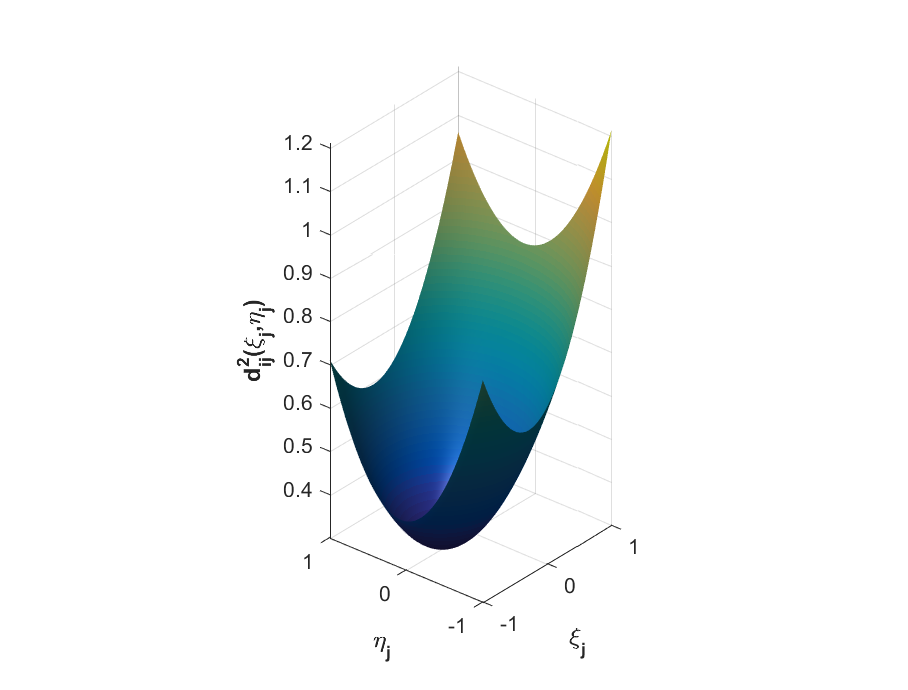
\includegraphics[width=0.5\textwidth]{images/Ch1/distance_squared.eps}
          } 
          \subfloat[Minimal distance configuration for a bi-linear quad element\label{fig.8b}]{%
            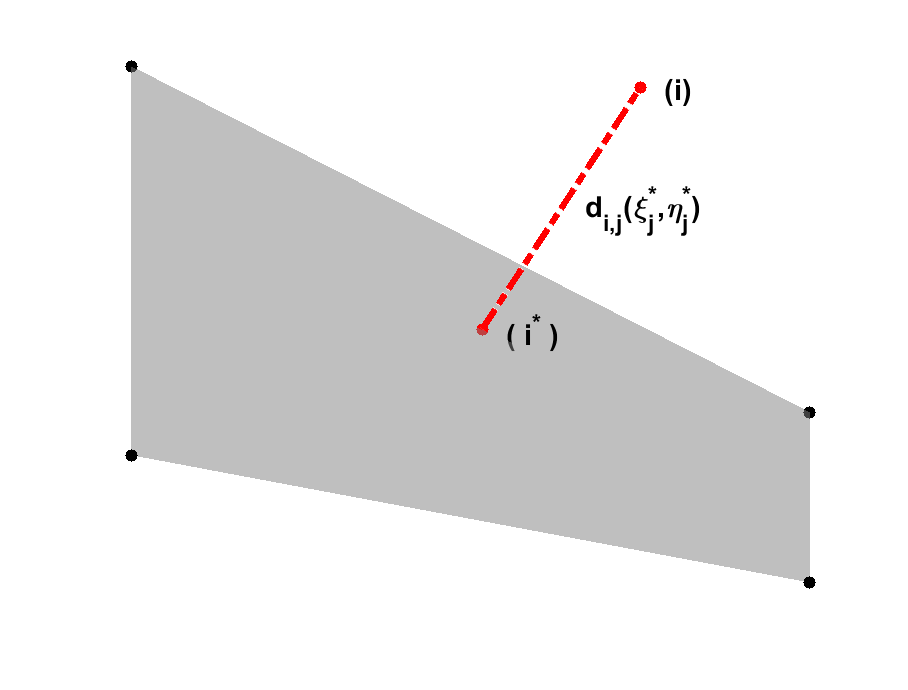
\includegraphics[width=0.5\textwidth]{images/Ch1/projection}
          }
          \caption{Node to element projection}
          \label{fig.8}
        \end{figure}
     When this procedure is used, for convex interface meshes there may be nodes that are far from the element $(j)$ but  that have their corresponding point $(i^*)$ inside the element $(j)$. The shape function of equation \eqref{eq.42} should take in account the minimal distance $d_{ij}\left(\xi^*_j,\eta^*_j \right)$: all the DOFs of the node $(i)$ at a distance superior to a given tolerance $t$ to its projection  $ (i^*) $ on $ \Gamma_j $ , should not be considered dependent on the $ (j) $ elements DOFs i.e.:
     \begin{equation}
     \label{eq.46}
     \Pi_{21i,j}=\begin{cases}\MatrixVar{N}_{j}^{\Gamma_1}\left(\xi^*,\eta^* \right) & d_{ij}\left(\xi^*_j,\eta^*_j \right)\leq t\\
     0 & \text{otherwise}.
     \end{cases}
     \end{equation}
\subsubsection{Weighted Residual Methods (WRM)}\label{sssec334}
The methods described until now are based on a strong formulation of the continuity on the interface of the displacement field (equation \eqref{eq.28}). On the other hand, segment to segment methods try to impose the continuity of displacements at the interface by the use of a weak form. One such method is the Weighted residual methods described in De Boer et al. \cite{de2007review}, Cebral{\=I} et al \cite{cebrali1997conservative} and  L{\"o}hner et al. \cite{lohner1998fluid} for the fluid-structure interaction problem.\footnote{These approaches do not make the use of Lagrange multipliers like in the Mortar methods (\cite{bernardi1989new},\cite{bernardi1993domain}); anyway when the shape functions of Lagrange multipliers are the same of the displacement field of the slave surface, the consequent equations are the same as it is also shown in Jeon et al. \cite{jeong2017element}} In this approach the jump of the displacement field across the interface has to be orthogonal in the $\mathbb{L}_2$ sense to the trace on $\Gamma_2$ of the kinematic admissible virtual displacement $\VectorVar{v} \in \mathbb{V}$:
\begin{equation}
\label{eq.47}
\begin{array}{cc}
  \int_{\Gamma}{\VectorVar{v}(\VectorVar{x})\cdot\left(\VectorVar{u}_{\Gamma_2}(\VectorVar{x})-\VectorVar{u}_{\Gamma_1}(\VectorVar{x}) \right)d\Gamma}=0 & \forall \VectorVar{v} \in \mathbb{V}    
\end{array}
\end{equation}
Discretizing $\VectorVar{v}(\VectorVar{x})$ using the shape functions of $\Gamma_2$  and using equation \eqref{eq.1.11} for each sub-domains and writing one equation for each shape function of the discretized space $\mathbb{V}^h_{\Gamma_2}$ equation \eqref{eq.47} becomes :
\begin{equation}
\label{eq.48}
\MatrixVar{M}_2\VectorVar{u}_{\Gamma_2}-\MatrixVar{M}_{21}\VectorVar{u}_{\Gamma_1}=\VectorVar{0}
\end{equation}
where the mass matrices are defined as:
\begin{eqnarray}
\label{eq.49}
M_{2i,j}=\int_{\Gamma}\MatrixVar{N}_{i}^{\Gamma_2}(\VectorVar{x})\cdot\MatrixVar{N}_{j}^{\Gamma_2}(\VectorVar{x})d\Gamma\\
\label{eq.50}
M_{21i,j}=\int_{\Gamma}\MatrixVar{N}_{i}^{\Gamma_2}(\VectorVar{x})\cdot\MatrixVar{N}_{j}^{\Gamma_1}(\VectorVar{x})d\Gamma
\end{eqnarray}
We can finally explicit the slave DOFs as a function of the master DOFs as:
\begin{equation}
\label{eq.51}
\VectorVar{u}_{\Gamma_2}=\MatrixVar{M}_2^{-1}\MatrixVar{M}_{21}\VectorVar{u}_{\Gamma_1}=\MatrixVar{\Pi}_{21}\VectorVar{u}_{\Gamma_1}
\end{equation}
It is shown in De Boer et al. \cite{de2007review}  that this method respects the condition of equation \eqref{eq32}, therefore the force resultant is conserved at the interface.
In order to evaluate the integral from equation \eqref{eq.49} and \eqref{eq.50} the support of the integral has to be chosen.

 \begin{figure}[!ht]
 \centering
     \subfloat[ Elements belonging to inconsistent meshes of the same  interface surface.\label{fig.9a}]{%
       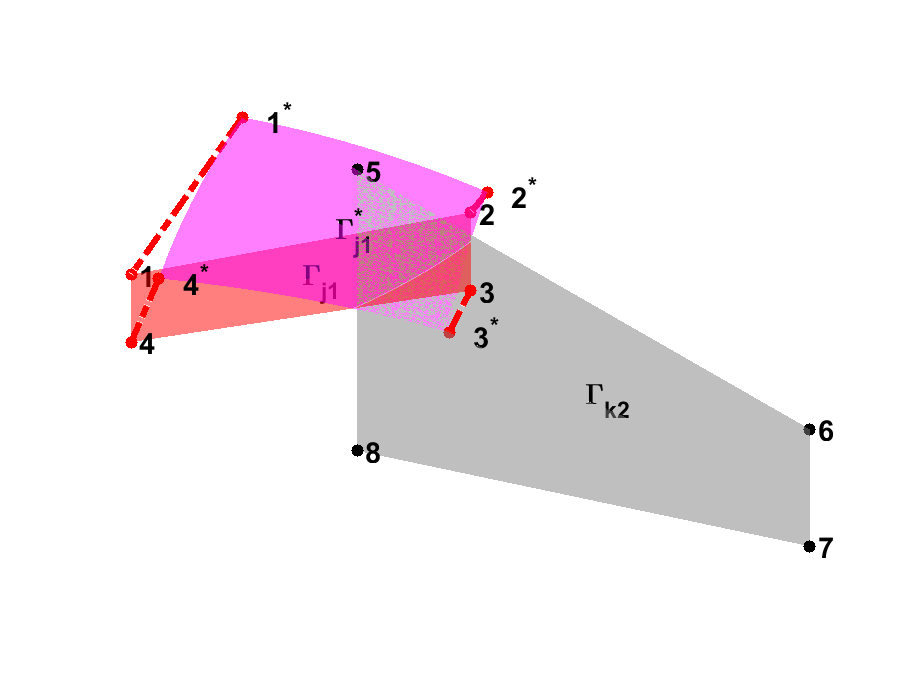
\includegraphics[width=0.6\textwidth]{images/Ch1/elementproj3}
     } \\
     \subfloat[ Projected master element on slave element  surface in slave local coordinates.\label{fig.9b}]{%
       \includegraphics[width=0.75\textwidth]{images/Ch1/projected_element}
     }
 
  
  \caption{Element to element projection examples. The master element surface $\Gamma_{j1}$ has been projected on the slave element surface $\Gamma_{k2}$ using the same procedure shown in figure (\ref{fig.8}) for each node of the element $j1$ ($1,2,3,4$). In this way it is possible to obtain the projected slave surface $\Gamma_{j1}^*$ ($1^*,2^*,3^*,4^*$). The union of the projection of all the elements of $\Gamma_1$ on $\Gamma_2$ is then indicated as $\Gamma_1^*$. After this projection, a change in local variables $(\xi_{k2},\eta_{k2})$ of the element $k2$ can be employed for the evaluation of Mass matrices (equations \eqref{eq.49} and \eqref{eq.50})}
  \label{fig.9}
\end{figure}
In fact in the most general case the surfaces described by the meshes will not be coincident and a projection will be needed (cf. figure (\ref{fig.9})) \footnote{Note that $\Gamma_{j1}^*$ sides are generally curved, in this work they are considered to be straight; this approximation will affect the accuracy of the evaluation of $ \mathbf{M_{21}}$ in equation \eqref{eq.50}. Nevertheless the error induced by this approximation can be considered negligible.}
\begin{figure}[!ht]
\centering
     \subfloat[ $N_{3^*}(\xi_{k2},\eta_{k2})$\label{fig.10a}]{%
       \includegraphics[width=0.3\textwidth]{images/Ch1/N3star}
     }
     \subfloat[  $N_{5}(\xi_{k2},\eta_{k2})$\label{fig.10b}]{%
       \includegraphics[width=0.3\textwidth]{images/Ch1/N5}
     }
     \subfloat[ $N_{3^*}(\xi_{k2},\eta_{k2})\cdot N_{5}(\xi_{k2},\eta_{k2})$\label{fig.10c}]{%
       \includegraphics[width=0.3\textwidth]{images/Ch1/N3sN5}
     }
     \caption{Shape function of node $3^*$ of $j1$, of node $5$ of $k2$ for the example of figure \ref{fig.9} and their product that has to be integrated in equation  \eqref{eq.50}, are represented.}
     \label{fig.10}
   \end{figure}
   \\
   One can observe that the integrand's support (cf. figure \ref{fig.10c}) is $\Gamma_{j1^*k2}\equiv \Gamma_{j1^*} \cap  \Gamma_{k2} $. The total support $\Gamma$ is therefore the union of all the intersections of each $\Gamma_{k2}$ with all corresponding projections $\Gamma_{j1^*}$ of $\Gamma_{j1}$ on $\Gamma_{k2}$:\\
\begin{equation}
\label{eq.52}
\Gamma\equiv\cup_{k2=1}^{N^{(e)}_2}\cup_{j1=1}^{N^{(e)}_1}\Gamma_{j1^*k2}
\end{equation}
 For the numeric evaluation of $\MatrixVar{M}_2$ and $\MatrixVar{M}_{21}$ we were inspired by the procedure in Puso et al. \cite{puso20043d}. Compared to Puso's original approach we implemented however some modifications in terms of node-to-element projection, and in terms of intersection polygon definition in order to render the procedure more robust. Instead of using the clipping algorithm of Foley \cite{foley1996computer} that may fail in some cases ( see \cite{gander2013algorithm} for further details), we implemented the procedure described by Gander et al. in \cite{gander2013algorithm}.
 To obtain the intersection polygon $\Gamma_{j1^*k2}$, firstly the nodes $(s1)$ of $\Gamma_{j1}$ that have a projection inside the element $(k2)$ are found.
Secondly the nodes $(s2)$ of $\Gamma_{k2}$ that are inside the projected element surface $\Gamma_{j1^*}$ are found.
Thirdly the intersection points $(s3)$ of all the sides of $\Gamma_{k2}$ with the one of $\Gamma_{j1^*}$ is carried out. The union of $(s1),(s2)$ and $(s3)$ form the vertices of the intersection polygon see figure \ref{fig.11a}.
\\
\begin{figure}[!ht]
     \subfloat[ Determination of $\Gamma_{j1^*k2}$ vertices. \label{fig.11a}]{%
       \includegraphics[width=0.5\textwidth]{images/Ch1/intersection_polygon}
     }
     \subfloat[  Integration over $\Gamma_{j1^*k2}$\label{fig.11b}]{%
       \includegraphics[width=0.5\textwidth]{images/Ch1/Gauss_point.eps}
     }
     \caption{Procedure for the determination of  $\Gamma_{j1^*k2}$ vertices and consequent numerical integration }
     \label{fig.11}
   \end{figure}
A triangulation of this polygon is obtained connecting all the sides with the polygon center. Finally, 3 Gauss points per triangle have to be used for the numerical integration of equation \eqref{eq.49} and \eqref{eq.50}) (see the example of figure \ref{fig.11b}). The Gauss point local coordinates  $(\VectorVar{\Xi}_{k2}^{(GP)},\VectorVar{\Theta}_{k2}^{(GP)})$ are easy to find as a function of the triangulation coordinates. On the other hand, to know the value of $\MatrixVar{N}_{j}^{\Gamma_1}$ on the corresponding points of $\Gamma_{j1^*}$ for equation \eqref{eq.50}), the local coordinates  $(\VectorVar{\Xi}_{j1}^{(GP)},\VectorVar{\Theta}_{j1}^{(GP)})$  have to be determined. Puso suggested even for this projection to use the normal of element ($k2$) on the center of the element. To be completely rigorous one should evaluate the normal to the surface $\Gamma_{k2}$ in each Gauss point and then make an intersection of the line on which the normal lies and the surface of $\Gamma_{j1}$ to finally have the local coordinates $(\VectorVar{\Xi}_{j1}^{(GP)},\VectorVar{\Theta}_{j1}^{(GP)})$ . In other words we should find the roots of the nonlinear system of equations:
\begin{multline}
\label{eq.53}
2\nabla\VectorVar{x}_{\Gamma_{k2}}\left(\VectorVar{\Xi}_{k2}^{(GP)},\VectorVar{\Theta}_{k2}^{(GP)}\right)\cdot \\ \cdot\left( \VectorVar{x}_{\Gamma_{k2}}\left(\VectorVar{\Xi}_{k2}^{(GP)},\VectorVar{\Theta}_{k2}^{(GP)}\right)-\VectorVar{x}_{\Gamma_{j1}}\left(\VectorVar{\Xi}_{j1}^{(GP)},\VectorVar{\Theta}_{j1}^{(GP)}\right)\right)= \VectorVar{0}
\end{multline}
Taking in consideration the fact that the sides of $\Gamma_{j1^*}$ are considered as straight segment between the projection on  $\Gamma_{k2}$ of the nodes of $(j1)$, even if this is not always the case, the use of equation \eqref{eq.53} is not recommended. Some Gauss points when re-projected on $\Gamma_{j1}$ could lie outside the element $(j1)$. To avoid this situation a geometric isoparametric interpolation between the local coordinate $(\xi_{j1},\eta_{j1})$ and the projected one $(\xi_{k2},\eta_{k2})$ is considered here:
\begin{eqnarray}
\label{eq.54}
\begin{aligned}
\xi_{k2}\left(\xi_{j1},\eta_{j1}\right)=\xi_{k2}^{1^*}N_1\left( \xi_{j1},\eta_{j1}\right)+\xi_{k2}^{2^*}N_2\left( \xi_{j1},\eta_{j1}\right)+\xi_{k2}^{3^*}N_3\left( \xi_{j1},\eta_{j1}\right)+\xi_{k2}^{4^*}N_4\left( \xi_{j1},\eta_{j1}\right)
\end{aligned} \\
\label{eq.55}
\begin{aligned}
\eta_{k2}\left(\xi_{j1},\eta_{j1}\right)=\eta_{k2}^{1^*}N_1\left( \xi_{j1},\eta_{j1}\right)+\eta_{k2}^{2^*}N_2\left( \xi_{j1},\eta_{j1}\right)+\eta_{k2}^{3^*}N_3\left( \xi_{j1},\eta_{j1}\right)+\eta_{k2}^{4^*}N_4\left( \xi_{j1},\eta_{j1}\right) 
\end{aligned} 
\end{eqnarray}
Where $(\xi_{k2}^{n^*},\xi_{k2}^{n^*})$ are the local coordinates of the projection of the n-th node of $(j1)$ on $\Gamma_{k2}$ and $N_n$ are the classic bilinear shape functions:
\begin{equation}
\begin{array}{cc}
\label{eq.56}
N_1\left( \xi_{j1},\eta_{j1}\right)=\frac{1}{4}\left( 1-\xi_{j1}\right)\left( 1-\eta_{j1}\right) \\ N_2\left( \xi_{j1},\eta_{j1}\right)=\frac{1}{4}\left( 1-\xi_{j1}\right)\left( 1+\eta_{j1}\right) \\
N_3\left( \xi_{j1},\eta_{j1}\right)=\frac{1}{4}\left( 1+\xi_{j1}\right)\left( 1+\eta_{j1}\right) \\ N_4\left( \xi_{j1},\eta_{j1}\right)=\frac{1}{4}\left( 1+\xi_{j1}\right)\left( 1-\eta_{j1}\right)
\end{array}
\end{equation}
Finally, equation \eqref{eq.54}-\eqref{eq.55} can be used to find $(\VectorVar{\Xi}_{j1}^{(GP)},\VectorVar{\Theta}_{j1}^{(GP)})$ solving another nonlinear system of equations:
\begin{eqnarray}
\label{eq.57}
\VectorVar{\Xi}_{k2}^{(GP)}-\xi_{k2}\left( \VectorVar{\Xi}_{j1}^{(GP)},\VectorVar{\Theta}_{j1}^{(GP)}\right)=\VectorVar{0} \\
\label{eq.58}
\VectorVar{\Theta}_{k2}^{(GP)}-\eta_{k2}\left( \VectorVar{\Xi}_{j1}^{(GP)},\VectorVar{\Theta}_{j1}^{(GP)}\right)=\VectorVar{0} 
\end{eqnarray}
This system can be solved numerically (e.g. with a Newton-Raphson algorithm) giving the analytical expression of the Jacobian matrix. In figure \ref{fig.12} the Gauss points are projected from $\Gamma_{j1*k2}$ back on $\Gamma_{j1}$ using the iso-parametric projection of equations \eqref{eq.57}-\eqref{eq.58}.
\begin{figure}[ht]
\centering
\includegraphics[width=8cm]{images/Ch1/PGproj}
\caption{Gauss point projection from $\Gamma_{j1*k2}$ back on $\Gamma_{j1}$ using the iso-parametric projection of equations \eqref{eq.57}-\eqref{eq.58}.}  
\label{fig.12}
\end{figure}
\subsection{Variational based approaches}\label{ssec34}
In variational approaches, instead of using the principle of virtual work to get the final system of equations, the displacement field solution of the static problem will be sought to minimize the total energy:
\begin{equation}
\label{eq.59}
E(\VectorVar{u})=\VectorVar{u}^T\MatrixVar{K}\VectorVar{u}-\VectorVar{u}^T\VectorVar{f}
\end{equation}
Considering the partition that we already introduced, the total energy becomes:
\begin{equation}
\label{eq.60}
\begin{aligned}
E( \VectorVar{u}_1,\VectorVar{u}_{\Gamma_1},\VectorVar{u}_{\Gamma_2},\VectorVar{u}_2
    )=\left\lbrace\begin{array}{cccc} \VectorVar{u}_1^T&\VectorVar{u}_{\Gamma_1}^T&\VectorVar{u}_{\Gamma_2}^T&\VectorVar{u}_2^T
    \end{array}\right\rbrace \\\left(\left[ \begin{array}{cccc} 
    \MatrixVar{K}_{1,1} & \MatrixVar{K}_{1,\Gamma_1} & \MatrixVar{0}& \MatrixVar{0} \\
   \MatrixVar{K}_{\Gamma_1,1} & \MatrixVar{K}_{\Gamma_1,\Gamma_1} & \MatrixVar{0}& \MatrixVar{0}\\ \MatrixVar{0}& \MatrixVar{0}& \MatrixVar{K}_{\Gamma_2,\Gamma_2}&\MatrixVar{K}_{\Gamma_2,2}\\   
    \MatrixVar{0} & \MatrixVar{0}& \MatrixVar{K}_{2,\Gamma_2} & \MatrixVar{K}_{2,2}\end{array} \right]\left\lbrace\begin{array}{c} \VectorVar{u}_1\\\VectorVar{u}_{\Gamma_1}\\\VectorVar{u}_{\Gamma_2}\\\VectorVar{u}_2
    \end{array}\right\rbrace
    -\left\lbrace\begin{array}{c} \VectorVar{f}_1\\\VectorVar{f}_{\Gamma_1}\\\VectorVar{f}_{\Gamma_2}\\\VectorVar{f}_2
    \end{array}\right\rbrace\right)
\end{aligned}
\end{equation}
Note that in equation \eqref{eq.60} the work at the interface of the residual is eliminated for energy conservation. The system of equations that comes from this formulation has a singular matrix, so that the solution of the static problem cannot be simply obtained by minimizing the total energy.
\subsubsection{Mortar Element Method}\label{sssec341}
The basic idea of the Mortar approach is to add a dislocation potential to the total energy, in order to impose the continuity of the displacement field at the interface:
\begin{equation}
\label{eq.61}
E_d\left( \VectorVar{u}, \VectorVar{\lambda} \right)=\int_{\Gamma} \VectorVar{\lambda}\left(\VectorVar{u}|_{\Gamma_1}-\VectorVar{u}|_{\Gamma_2}\right)d\Gamma
\end{equation}
This potential is summed with the total energy to get the Lagrangian functional $E_l \left(\VectorVar{u}, \VectorVar{\lambda} \right)=E_d\left( \VectorVar{u}, \VectorVar{\lambda} \right)+E(\VectorVar{u})$ whose stationary points are the solution of the constrained optimization:
\begin{equation}
\label{eq.62}
\left\lbrace \begin{array}{c}
\min_{\VectorVar{u}}(E(\VectorVar{u}))\\
  \VectorVar{u}|_{\Gamma_1}-\VectorVar{u}|_{\Gamma_2}=0
\end{array}\right.
\end{equation}
Similarly to Master/Slave approaches, the mortar approach needs the choice of one surface to be the mortar surface and the other to be the non-mortar.
The interpolation functions of the Lagrangian multipliers $\VectorVar{\lambda}$ are (in the case of two domains) chosen to be the same as those of the slave surface:\footnote{In the work of Puso et al \cite{puso20043d} the dual space is also employed}
\begin{equation}
\label{eq.63}
\VectorVar{\lambda}(\VectorVar{x}|_{\Gamma_2})=\MatrixVar{N}(\VectorVar{x}|_{\Gamma_2})\VectorVar{\lambda}_{\Gamma_2}
\end{equation}
The dislocation potential can then be written as:
\begin{equation}
\label{eq.64}
E_d( \VectorVar{u}_{\Gamma_1},\VectorVar{u}_{\Gamma_2},\VectorVar{\lambda}_{\Gamma_2})=\VectorVar{\lambda}_{\Gamma_2}^T\left(\MatrixVar{M}_{21}\VectorVar{u}_{\Gamma_1}-\MatrixVar{M}_2\VectorVar{u}_{\Gamma_2}\right)
\end{equation}
Then the Lagrangian functional is stationary  for:
\begin{equation}
\label{eq.65}
 \left[ \begin{array}{ccccc} 
    \MatrixVar{\mathbf{K}}_{1,1} & \MatrixVar{\mathbf{K}}_{1,\Gamma_1} &\MatrixVar{0} &\MatrixVar{0}& \MatrixVar{0} \\
   \MatrixVar{\mathbf{K}}_{\Gamma_1,1} & \MatrixVar{\mathbf{K}}_{\Gamma_1,\Gamma_1} &\MatrixVar{M}_{21}^T & \MatrixVar{0}& \MatrixVar{0}\\ \MatrixVar{0} &\MatrixVar{M}_{21} &\MatrixVar{0} &-\MatrixVar{M}_{2}& \MatrixVar{0}\\\MatrixVar{0}& \MatrixVar{0}& -\MatrixVar{M}_{2}^T & \MatrixVar{\mathbf{K}}_{\Gamma_2,\Gamma_2} &\MatrixVar{\mathbf{K}}_{\Gamma_2,2}\\   
    \MatrixVar{0} & \MatrixVar{0}&\MatrixVar{0}& \MatrixVar{\mathbf{K}}_{2,\Gamma_2} & \MatrixVar{\mathbf{K}}_{2,2}\end{array} \right]\left\lbrace\begin{array}{c} \VectorVar{u}_1\\\VectorVar{u}_{\Gamma_1}\\\VectorVar{\lambda}_{\Gamma_2}\\\VectorVar{u}_{\Gamma_2}\\\VectorVar{u}_2
    \end{array}\right\rbrace=\left\lbrace\begin{array}{c} \VectorVar{f}_1\\\VectorVar{f}_{\Gamma_1}\\\VectorVar{0}\\\VectorVar{f}_{\Gamma_2}\\\VectorVar{f}_2
    \end{array}\right\rbrace
\end{equation}
Even if the equations obtained from this approach seem to be different from the one of the WRM, eliminating the Lagrange eigenvalues from equation \eqref{eq.65} we can recognize that they have the same solution (see Jeong et al. \cite{jeong2017element} for the proof). It can be noted that this method has the same difficulties of implementation and of evaluation cost encountered with the WRM method: The integral of the shape function over the intersection of the interface has to be evaluated in order to evaluate the mass matrices $\MatrixVar{M}_{21},\MatrixVar{M}_{2}$. The Mortar approach is shown to be as accurate as the WRM approach but with a noticeably longer effort due to the increased number of variables. For this reason in section \ref{sec4} only WRM has been implemented and compared with other methods.
\subsection{The Internodes Approach}\label{ssec35}
Here we describe the internodes approach, introduced by Deparis et al in \cite{deparis2016internodes} and further analyzed by Gervasio et al. in \cite{gervasio2016analysis}. We derived its matrix formulation directly from equation \eqref{eq.15}. Like in the elimination approaches the continuity of the displacement field is guaranteed by equation \eqref{eq.28}. On the other hand the balance of energy and force sum are not imposed. The forces $\VectorVar{t}_{12}$ and $\VectorVar{t}_{21}$ are supposed to be interpolated with the same shape functions of displacement  on each subdomain interface:
\begin{eqnarray}
\label{eq.66}
 \VectorVar{t}_{12}(\VectorVar{x}|_{\Gamma_2})=\MatrixVar{N}^{(h)}(\VectorVar{x}|_{\Gamma_2}) \VectorVar{p}_{2}\\
 \label{eq.67}
 \VectorVar{t}_{21}(\VectorVar{x}|_{\Gamma_1})=\MatrixVar{N}^{(h)}(\VectorVar{x}|_{\Gamma_1}) \VectorVar{p}_{1}
\end{eqnarray}
where $\VectorVar{p}_{1}$ and $\VectorVar{p}_{2}$ are the vector of internal forces per unit of surface interpolating $\VectorVar{t}_{12}(\VectorVar{x}|_{\Gamma_2})$ and $ \VectorVar{t}_{21}(\VectorVar{x}|_{\Gamma_1})$.
Conforming to these definitions the residual at the interface may be evaluated as:
\begin{eqnarray}
\label{eq.68}
 \VectorVar{r}_{\Gamma_1}=\int_{\Gamma_1}\MatrixVar{N}^{(h)}(\VectorVar{x}|_{\Gamma_1})\cdot\MatrixVar{N}^{(h)}(\VectorVar{x}|_{\Gamma_1}) \VectorVar{p}_{1}d\Gamma_1=\MatrixVar{M}_1\VectorVar{p}_{1}\\
 \label{eq.69}
\VectorVar{r}_{\Gamma_2}=\int_{\Gamma_2}\MatrixVar{N}^{(h)}(\VectorVar{x}|_{\Gamma_2})\cdot\MatrixVar{N}^{(h)}(\VectorVar{x}|_{\Gamma_2}) \VectorVar{p}_{2}d\Gamma_2=\MatrixVar{M}_2\VectorVar{p}_{2}
\end{eqnarray}
The balance of the internal forces per unit area is imposed in a similar fashion to the continuity of the displacements as in equation \eqref{eq.28}, but this time a second interpolation operator is used:
\begin{equation}
\label{eq.70}
\VectorVar{p}_{1}+\MatrixVar{\Pi}_{12}\VectorVar{p}_{2}=\VectorVar{0}
\end{equation}
Substituting equation \eqref{eq.68} and \eqref{eq.69} in \eqref{eq.70} one gets:
\begin{equation}
\label{eq.71}
\VectorVar{r}_{\Gamma_1}+\MatrixVar{M}_1\MatrixVar{\Pi}_{12}\MatrixVar{M}_2^{-1}\VectorVar{r}_{\Gamma_2}=\VectorVar{r}_{\Gamma_1}+\MatrixVar{Q}_{12}\VectorVar{r}_{\Gamma_2}=\VectorVar{0}
\end{equation}
Finally, using equations \eqref{eq.71} and \eqref{eq.28} in \eqref{eq.15} one can get:
\begin{equation}
\label{eq.72}
\begin{aligned}
\left[ \begin{array}{ccc} 
    \MatrixVar{\mathbf{K}}_{1,1} & \MatrixVar{\mathbf{K}}_{1,\Gamma_1} & \MatrixVar{0} \\
   \MatrixVar{\mathbf{K}}_{\Gamma_1,1} & \MatrixVar{\mathbf{K}}_{\Gamma_1,\Gamma_1}+ \MatrixVar{Q}_{12}\MatrixVar{\mathbf{K}}_{\Gamma_2,\Gamma_2}\MatrixVar{\Pi}_{21} & \MatrixVar{Q}_{12}\MatrixVar{\mathbf{K}}_{\Gamma_2,2}\\   
    \MatrixVar{0} & \MatrixVar{\mathbf{K}}_{2,\Gamma_2}\MatrixVar{\Pi}_{21} & \MatrixVar{\mathbf{K}}_{2,2}\end{array} \right] \left\lbrace \begin{array}{c} \VectorVar{u}_1\\\VectorVar{u}_{\Gamma_1}\\\VectorVar{u}_2
    \end{array}\right\rbrace= \left\lbrace\begin{array}{c} \VectorVar{f}_1\\\VectorVar{f}_{\Gamma_1}+\MatrixVar{Q}_{12}\VectorVar{f}_{\Gamma_2}\\\VectorVar{f}_2
    \end{array}\right\rbrace
    \end{aligned}
\end{equation}
It can be observed that the system of equations of the internodes formulation is not symmetric and that equations \eqref{eq.31} and \eqref{eq32} are not imposed, so that internodes does not conserve \textit{apriori} neither work nor resultants of forces and moments. On the other hand the formulation and the implementation are straightforward if compared with the mortar and the WRM approaches: only the mass matrices $\MatrixVar{M}_2$, $\MatrixVar{M}_1$ and the interpolation operators $\MatrixVar{\Pi}_{12}$ and $\MatrixVar{\Pi}_{21}$ are needed. Good convergence properties have been showed in the work of Gervasio et al. \cite{gervasio2016analysis}.
\subsection{Weighted Average Continuity Approach (WACA)}\label{sssec36}
The collocation approaches even if simple are not accurate enough when the most refined mesh is chosen as master surface. On the other hand the segment to segment approaches are very accurate but are complex and need much more computational effort. The Internodes approach seeks to achieve such a trade-off between complexity and accuracy but, as it will be shown in section \ref{sec4}, the fact that it does not conserve the resultant force vector and total energy at the interface can deteriorate its accuracy. In \cite{coniglio2018weighted} we proposed a new approach that shares with Internodes its simplicity but achieves an improved accuracy.
This one is based on another expression of the continuity of the displacement field at the interface. Before we introduce the new formulation let us highlight some equations that can be derived. Each line of the vector coming from the multiplication of the interface mass matrix and the interface displacement vector represents the integral over the interface of the displacement field times the shape function of the DOF corresponding to the selected line. We can define a weighted average displacement field using as weight the shape function:
\begin{equation}
\label{eq.73a}
\bar{u}_{\Gamma_1i}=\frac{\int_{\Gamma_1}\VectorVar{u}(\VectorVar{x}\|_{\Gamma_1})\cdot\MatrixVar{N}_{i}^{\Gamma_1}(\VectorVar{x}\|_{\Gamma_1})d\Gamma_1}{\int_{\Gamma_1(\MatrixVar{N}_{i}^{\Gamma_1}(\VectorVar{x}\|_{\Gamma_1}))_id\Gamma_1}}
\end{equation}
this can be reformulated as:
\begin{equation}
\label{eq.73}
({M}_{1}{u}_{\Gamma_1})_i=S_{N_i}\bar{u}_{\Gamma_1i}
\end{equation}
where $S_{N_i}$ is the integral of the i-th shape function over its support  and $\bar{u}_{\Gamma_1i}$ is the weighted average of the i-th displacement on $\Gamma_1$. 
We can put this relationship in the matrix form:
\begin{eqnarray}
\label{eq.74}
\MatrixVar{M}_{1}\VectorVar{u}_{\Gamma_1}=\MatrixVar{S}_1\VectorVar{\bar{u}}_{\Gamma_1}\qquad
\MatrixVar{M}_{2}\VectorVar{u}_{\Gamma_2}=\MatrixVar{S}_2\VectorVar{\bar{u}}_{\Gamma_2}
\end{eqnarray}
where we denote with $\MatrixVar{S}_1$ and $\MatrixVar{S}_2$ the diagonal matrices containing on the diagonal the integral of each shape function on its support\footnote{$\MatrixVar{S}_1$ and $\MatrixVar{S}_2$ are also denoted as lumped mass matrices}, and with $\VectorVar{\bar{u}}_{\Gamma_1}$ and $\VectorVar{\bar{u}}_{\Gamma_2}$ the weighted average displacement field of each component over the corresponding shape function support.
In the approach we propose we seek to state the continuity of the weighted average displacement interpolating between the two surfaces i.e.
\begin{equation}
\label{eq.75}
\VectorVar{\bar{u}}_{\Gamma_2}=\MatrixVar{\Pi}_{21}\VectorVar{\bar{u}}_{\Gamma_1}
\end{equation}
By substitution of equation \eqref{eq.74}  into equation  \eqref{eq.75} one gets a new interpolation operator between the displacement fields:
\begin{equation}
\label{eq.76}
\VectorVar{u}_{\Gamma_2}=\MatrixVar{M}_{2}^{-1}\MatrixVar{S}_2\MatrixVar{\Pi}_{21}\MatrixVar{S}_1^{-1}\MatrixVar{M}_{1}\VectorVar{u}_{\Gamma_1}=\MatrixVar{\Pi}_{21}^{*}\VectorVar{u}_{\Gamma_1}
\end{equation}
If the interpolation operator $\MatrixVar{\Pi}_{21}$ satisfies the conservation conditions given by equation \eqref{eq32}, $\MatrixVar{\Pi}^{*}_{21}$ will also satisfy the same conditions:
\begin{equation}
\label{eq.77}
\begin{aligned}
\MatrixVar{\Pi}_{21}^{*}\MatrixVar{1}_{\Gamma_1}=\MatrixVar{M}_{2}^{-1}\MatrixVar{S}_2\MatrixVar{\Pi}_{21}\MatrixVar{S}_1^{-1}\MatrixVar{M}_{1}\MatrixVar{1}_{\Gamma_1}=\MatrixVar{M}_{2}^{-1}\MatrixVar{S}_2\MatrixVar{\Pi}_{21}\MatrixVar{S}_1^{-1}\MatrixVar{S}_1\MatrixVar{1}_{\Gamma_1}=\\=
\MatrixVar{M}_{2}^{-1}\MatrixVar{S}_2\MatrixVar{\Pi}_{21}\MatrixVar{1}_{\Gamma_1}=\MatrixVar{M}_{2}^{-1}\MatrixVar{S}_2\MatrixVar{1}_{\Gamma_2}=\MatrixVar{M}_{2}^{-1}\MatrixVar{M}_{2}\MatrixVar{1}_{\Gamma_2}=\MatrixVar{1}_{\Gamma_2}
\end{aligned}
\end{equation}
where we used twice the fact that the mass coherent and lumped mass matrices conserve the sum of lines i.e.
\begin{eqnarray}
\label{eq.78}
\MatrixVar{M}_{1}\MatrixVar{1}_{\Gamma_1}=\MatrixVar{S}_{1}\MatrixVar{1}_{\Gamma_1} \qquad \MatrixVar{M}_{2}\MatrixVar{1}_{\Gamma_2}=\MatrixVar{S}_{2}\MatrixVar{1}_{\Gamma_2} 
\end{eqnarray}
The condition of zero work at the interface (equation \eqref{eq.29}) can be used as was done in the classic elimination methods so that the final matrix form of the WACA approach is:
\begin{equation}
\label{eq.79}
\begin{aligned}
\left[ \begin{array}{ccc} 
    \MatrixVar{\mathbf{K}}_{1,1} & \MatrixVar{\mathbf{K}}_{1,\Gamma_1} & \MatrixVar{0} \\
   \MatrixVar{\mathbf{K}}_{\Gamma_1,1} & \MatrixVar{\mathbf{K}}_{\Gamma_1,\Gamma_1}+ (\MatrixVar{\Pi}_{21}^{*})^T\MatrixVar{\mathbf{K}}_{\Gamma_2,\Gamma_2}\MatrixVar{\Pi}_{21}^* & (\MatrixVar{\Pi}_{21}^{*})^T\MatrixVar{\mathbf{K}}_{\Gamma_2,2}\\   
    \MatrixVar{0} & \MatrixVar{\mathbf{K}}_{2,\Gamma_2}\MatrixVar{\Pi}^{*}_{21} & \MatrixVar{\mathbf{K}}_{2,2}\end{array} \right] \left\lbrace \begin{array}{c} \VectorVar{u}_1\\\VectorVar{u}_{\Gamma_1}\\\VectorVar{u}_2
    \end{array}\right\rbrace=\\ \left\lbrace\begin{array}{c} \VectorVar{f}_1\\\VectorVar{f}_{\Gamma_1}+(\MatrixVar{\Pi}_{21}^{*})^T\VectorVar{f}_{\Gamma_2}\\\VectorVar{f}_2
    \end{array}\right\rbrace
\end{aligned}
\end{equation}
This formulation shares the same simplicity of the Internodes approach, on the other hand satisfies \textit{\textit{a priori}} the conservation of the residual sum at the interface and of the energy at the interface.  

\subsection{\textit{A priori} conservation of moments}\label{ssec37}
All the methods proposed here do respect the balance of residual resultant and residual work but do not respect an \textit{a priori} condition on the moments of the resultant at the interface. In the work of Puso \cite{puso20043d}, to enforce this balance of moments and keep the same formulation of the mortar method the nodes of the slave surface in the undeformed configuration are moved on the interface surface. This method is interesting but still not very practical to conserve the meshes of both sub-domains. Another interesting approach is proposed by  Park et al. in \cite{park2002simpl}, were a third surface and mesh (the frame) are introduced and the balance of moments and of the patch test are satisfied choosing the position of nodes on the frame. To the authors' best knowledge no works exist which propose to satisfy the moments' balance equation through an \textit{a priori} condition on the interpolation operators $\Pi_{12}$, $\Pi_{21}$. This is the objective of this subsection in which a necessary condition is determined and used to correct the projection operator for all eliminations methods as well as for the new WACA method.
First of all let’s write the balance of moments of the residual:
\begin{equation}
\label{eq.80}
\sum_{i=1}^{n_{\Gamma_1}}\VectorVar{OP}_{i\Gamma_1}\times \VectorVar{R}_{i\Gamma_1}+\sum_{j=1}^{n_{\Gamma_2}}\VectorVar{OP}_{j\Gamma_2}\times \VectorVar{R}_{j\Gamma_2}=\VectorVar{0}
\end{equation}
We defined here $\VectorVar{OP}_{i\Gamma_s}$ as the vector connecting the fixed point O to the positions of the $i^{th}$ nodes of the $\Gamma_s$ surface (s=1,2); $\VectorVar{R}_{i\Gamma_s}$ as the vector of the residual force at the same node. This equation must be satisfied for each possible combination of residuals. For the energy balance \eqref{eq.31} the residuals are not independent so that all the combinations of residuals can be obtained as all the vectors in $\VectorVar{R}^{N_{\Gamma_2}}$ where $N_{\Gamma_2}=n_d n_{\Gamma_2}$ is the number of DOFs of the second interface. Satisfying equation \eqref{eq.80} for all vectors of $\VectorVar{R}^{N_{\Gamma_2}}$ means that it has to be verified for each vector in a normal basis, for example the canonical one.
For each node $j$ and for each direction $n_d^{(j)}$ (for each $k_2$ DOF) we can then write 3 equations as follows: 
\begin{eqnarray}
\label{eq.80b}
\begin{aligned}
\sum_{i=1}^{n_{\Gamma_1}}\VectorVar{OP}_{i\Gamma_1}\times (\VectorVar{R}_{i\Gamma_1})_{n_d^{(i)}}+\VectorVar{OP}_{j\Gamma_2}\times (\VectorVar{R}_{j\Gamma_2})_{n_d^{(j)}}=\VectorVar{0} \quad \forall k_2\in \lbrace1,2,\dots,N_{\Gamma_2} \rbrace
\end{aligned}
\end{eqnarray}
By the use of \eqref{eq.31} on can replace $(\VectorVar{R}_{i\Gamma_1})_{n_d^{(i)}}$ by the $(k_2,\VectorVar{k_1})$ terms of $\MatrixVar{\Pi}_{21}$ , that we will denote here as $\left(\VectorVar{\Pi_{21}}\right)_{(k_2,\VectorVar{k_1})}$, where   $\VectorVar{k_1}$ are the indexes of the DOFs of the $i^{th}$ node of $\Gamma_1$. Choosing $O \equiv P_{j\Gamma_2} $ to write each moment equation, equation \eqref{eq.80b} becomes:
\begin{eqnarray}
\label{eq.80c}
\begin{aligned}
\sum_{i=1}^{n_{\Gamma_1}}\VectorVar{P_{j\Gamma_2}P_{i\Gamma_1}}\times \left(\VectorVar{\Pi_{21}}\right)_{(k_2,\VectorVar{k_1})}^T=\VectorVar{0} \quad \forall k_2\in \lbrace1,2,\dots,N_{\Gamma_2} \rbrace
\end{aligned}
\end{eqnarray}
This equation can be also written in the following matrix form:
\begin{eqnarray}
\label{eq.80d}
\left(\VectorVar{\Pi_{21}}\right)_{k_2}\cdot\MatrixVar{B}_{k2}=\VectorVar{0} \qquad \forall k_2\in \lbrace1,2,\dots,N_{\Gamma_2} \rbrace
\end{eqnarray}
Where $\left(\VectorVar{\Pi_{21}}\right)_{k_2}$ is the $k_2^{th}$ line of $\MatrixVar{\Pi}_{21}$, $\MatrixVar{B}_{k2}$ is a matrix $N_{\Gamma_1}\times3$ defined by:
\begin{eqnarray}
\label{eq.80e}
(\MatrixVar{B}_{k2})_{(k_1,n_d)}=(\VectorVar{P_{j\Gamma_2}P_{i\Gamma_1}}\times\VectorVar{n_d}^{(k_1)})_{n_d}
\end{eqnarray}
 $\VectorVar{n_d}^{(k_1)}$ is the $3\times1$ versor of the $k_1^{th}$ DOF direction and by $(\bullet)_{n_d}$ the extraction of the  ${n_d}$ component of a vector. Equation \eqref{eq.80d} and equation \eqref{eq32} form a system of 6 equations for each line of the projecting operator that can be compactly written as:
 \begin{equation}
 \label{eq.80f}
 \left(\VectorVar{\Pi_{21}}\right)_{k_2}\cdot\MatrixVar{A}_{k_2}^T=\left(\VectorVar{\Pi_{21}}\right)_{k_2}\cdot\left[
 \begin{array}{c c}
   \MatrixVar{1}_{\Gamma_1}&
   \MatrixVar{B}_{k2}
 \end{array}
 \right]=\left[\begin{array}{c c}
   \left(\VectorVar{1_{\Gamma_2}}\right)_{k_2}&
   \VectorVar{0}
 \end{array}
 \right]=\VectorVar{b}^T
 \end{equation}
 We seek to correct the projection operator coming from an elimination approach (RBF, WRM, WACA) to respect equation \eqref{eq.80f}. Since we do not want to significantly modify the previous interpolations, we would like to have a new line  $ \left(\VectorVar{\Pi_{21}}\right)_{k_2}^{(c)}$ that is as close as possible to the original one  $ \left(\VectorVar{\Pi_{21}}\right)_{k_2}$ and that satisfies equation \eqref{eq.80f}. In other terms we want to solve the optimization problem
 \begin{equation}
 \label{eq.80g}
\left\lbrace \begin{array}{c}
 min_{\VectorVar{s}}\left(\VectorVar{s}-\left(\VectorVar{\Pi_{21}}\right)_{k_2} \right)^T\cdot\left(\VectorVar{s}-\left(\VectorVar{\Pi_{21}}\right)_{k_2} \right)\\
 \VectorVar{s}\cdot\MatrixVar{A}_{k_2}^T=\VectorVar{b}^T
 \end{array} \right.
 \end{equation}
 Here we indicated $ \left(\VectorVar{\Pi_{21}}\right)_{k_2}^{(c)}$ as $\VectorVar{s}$ for brevity. To solve this constrained optimization problem the Lagrangian approach can be used. The stationary condition of the Lagrangian form a linear system of equations that can be solved to find  $\VectorVar{s}^T$ is:
 \begin{equation}
 \label{eq.80h}
\left(\left(\VectorVar{\Pi_{21}}\right)_{k_2}^{(c)}\right)^T=\left(\VectorVar{\Pi_{21}}\right)_{k_2}^T+\MatrixVar{A}_{k_2}^T\cdot(\MatrixVar{A}_{k_2}\cdot\MatrixVar{A}_{k_2}^T)^{-1}(\VectorVar{b}-\MatrixVar{A}_{k_2}\cdot\left(\VectorVar{\Pi_{21}}\right)_{k_2}^T)
 \end{equation}
 The resulting operator $\MatrixVar{\Pi}_{21}^{(c)}$ will then respect both the balance of resultant of residual/energy and moments. Still, its precision in terms of displacement and stress continuity could be affected, so in the next section we will analyze its numerical efficiency. The correction presented here can be adapted even for the Internodes approach. The corrected scheme will modify the column of the $\MatrixVar{Q}_{12}$ and not the line of $\MatrixVar{\Pi}_{21}$. The resulting scheme will therefore conserve the balance  of forces and moments but not of energy since $\MatrixVar{Q}_{12}^{(c)}\neq\MatrixVar{\Pi}_{21}^T$.
 \subsection{Benchmarking on numerical test cases}\label{sec4}
 \subsubsection{Test cases definition and analysis for consistent meshes}\label{ssec41}
 In this section we present two test case geometries, each investigated under pure traction and bending-traction boundary conditions, which will serve for benchmarking various methods considered. The first case is a column like structure with spherical ends see figure \ref{fig.13a}. In the second case (figure \ref{fig.13b}) the bottom structure is wider and shorter than the upper one and both ends are spherical. Both structures are completely fixed at the bottom face and for the pure traction loading they are loaded on the upper surface with a constant surface traction in the z direction of magnitude 30.25 MPa. The analysis made for configuration (1) is actually very similar to the ones frequently studied in the literature (cf. \cite{song2017virtual}). The main differences consist in the clamping on the bottom side and in curved instead of planar upper and bottom faces. Hence our test does not have a closed form solution and we had to consider the fine and consistent mesh as reference for the analysis. One should also keep in mind that none of the presented methods passes linear patch tests for curved interfaces. Anyway classic constant stress patch test is not a necessary condition for optimality convergence \cite{stummel1980limitations}, other conditions have to be fulfill like in the Generalized patch test \cite{stummel1979generalized} or in the FEM test \cite{shi1987fem} . On the other hand one could be wondering how much the error induced by the violation of the patch test can affect a general solution. The following benchmarking will try to bring some insights to this question.\\
 In the FEM, the upper and the lower domains are meshed with linear brick finite elements with complete quadrature (8 Gauss points). In configuration (1) in figure \ref{fig.13a} the upper and the lower domains are meshed with $10\times10\times10$ and $10\times10\times20$ elements respectively. Configuration (1) represents a very simple configuration and we also sought a more general case in which the interface surfaces do not have the same boundaries. To achieve this we considered configuration (2), see figure \ref{fig.13b}. In this case the nodes that are not inside the boundary of the intersection of the interface surfaces have to be eliminated from the interface node set. To find these nodes one has to check the interpolation operator (applicable for RL-RBF but also for ES) looking for all-zero column and all-zero lines and eliminate the corresponding nodes from the set of interface node. This avoids major errors of projection and gives much better results for all the methods considered. In configuration (2) in figure \ref{fig.13b} the upper domain is meshed in the same way and the lower domain with $20\times20\times5$ elements. The total active DOFs are 10890 in configuration (1) and 10245 in configuration (2). These configurations are denoted in the rest of this paper as reference configurations and will serve for comparison, since they involve consistent meshes between the upper and lower domains and involve the most refined meshes.
 \begin{figure}[!ht]
 \centering
      \subfloat[Geometric configuration (1) \label{fig.13a}]{%
      \adjincludegraphics[width=0.35\textwidth,trim={{.4\width} {.27\height} {.35\width} {.15\height} },clip]{images/Ch1/scenario2}
      }
      \subfloat[Geometric configuration (2)  \label{fig.13b}]{%
      \adjincludegraphics[width=0.35\textwidth,trim={{.4\width} {.27\height} {.35\width} {.15\height} },clip]{images/Ch1/scenario4}
      }
      \caption{Geometric configurations (1) and (2), pure traction load case }
      \label{fig.13}
    \end{figure}
 \\
 In figure \ref{fig.14} a bending-traction loading condition is applied to both geometrical configurations. In this case we simply added a second surface traction component in the x direction with the same magnitude as the one in z direction (30.25MPa).
 \begin{figure}[!ht]
 \centering
      \subfloat[Geometric configuration (1)  \label{fig.14a}]{%
      \adjincludegraphics[width=0.35\textwidth,trim={{.3\width} {.1\height} {.35\width} {.1\height} },clip]{images/Ch1/scenario2B}
      }
      \subfloat[Geometric configuration (2)  \label{fig.14b}]{%
      \adjincludegraphics[width=0.35\textwidth,trim={{.4\width} {.27\height} {.35\width} {.15\height} },clip]{images/Ch1/scenario4b}
      }
      \caption{Geometric configurations (1) and (2), bending-traction traction load case }
      \label{fig.14}
    \end{figure}
 The upper and the lower domains are meshed with consistent meshes, so that this analysis does not introduce any interpolation error between the meshes. The displacement field corresponding to the pure traction and to the bending-traction loadings are represented in figure \ref{fig.15} and \ref{fig.16} respectively.
 \\
    \begin{figure}[!ht]
    \centering
      \subfloat[Geometric configuration (1) \label{fig.15a}]{%
      \adjincludegraphics[width=0.35\textwidth]{images/Ch1/displacement_magnitude2}
      }
      \subfloat[Geometric configuration (2) \label{fig.15b}]{%
      \adjincludegraphics[width=0.35\textwidth]{images/Ch1/displacement_magnitude4}
      }
      \caption{Displacement amplitude under pure traction load case }
      \label{fig.15}
    \end{figure}
    \begin{figure}[!ht]
    \centering
      \subfloat[Geometric configuration (1) \label{fig.16a}]{%
      \adjincludegraphics[width=0.35\textwidth]{images/Ch1/displacement_magnitude2b}
      }
      \subfloat[Geometric configuration (2) \label{fig.16b}]{%
      \adjincludegraphics[width=0.35\textwidth]{images/Ch1/displacement_magnitude4b}
      }
      \caption{Displacement amplitude under bending-traction load case }
      \label{fig.16}
    \end{figure}
    The finite element code (in house code, implemented in Matlab) used for this test has been tested and validated with a comparison with Abaqus 6.14.
    One can observe that in these configurations the displacement field is continuous at the interface between the upper and the lower domain. 
    To represent the Von Mises stress, that is evaluated at each Gauss integration point a global least square interpolation approach \cite{hinton1974local} was adopted  (cf. figure \ref{fig.17} and \ref{fig.18})\footnote{In such approach the value of von Mises stress is supposed to be interpolated by finite element shape functions. As the values of von Mises stress are computed at the Gauss points, a least square approach is adopted to determine the nodal values that minimize the difference between the interpolated von Mises stress and the computed ones at Gauss point locations.}. One can observe that for these meshes in both configurations the Von Mises stress is continuous at the interface. 
 \newpage
    \begin{figure}[!ht]
    \centering
      \subfloat[Geometric configuration (1)\label{fig.17a}]{%
      \adjincludegraphics[width=0.35\textwidth]{images/Ch1/VMstress2}
      }
      \subfloat[Geometric configuration (2) \label{fig.17b}]{%
      \adjincludegraphics[width=0.35\textwidth]{images/Ch1/VMstress4t}
      }
      \caption{Von Mises stress under pure traction load case}
      \label{fig.17}
    \end{figure}
    \begin{figure}[!ht]
    \centering
      \subfloat[Geometric configuration (1) \label{fig.18a}]{%
      \adjincludegraphics[width=0.35\textwidth]{images/Ch1/VMstress2B}
      }
      \subfloat[Geometric configuration (2) \label{fig.18b}]{%
      \adjincludegraphics[width=0.35\textwidth]{images/Ch1/VMstress4Bt}
      }
      \caption{Von Mises stress under bending-traction load case }
      \label{fig.18}
    \end{figure}
 \newpage
 \subsection{Benchmark Results}\label{ssec42}
 The inconsistent meshes that are tested here are obtained by changing the mesh of the bottom domain and keeping constant the mesh of the upper domain. The upper domain will always be a ($10\times10\times10$) domain, on the other hand the bottom domain will change its mesh as ($n\times n\times20$) for configuration (1) and as ($m \times m \times 5$) in the configuration (2), with $n$ and $m$ varying.
    \begin{figure}[!ht]
    \centering
      \subfloat[Geometric configuration (1) $n=4$ \label{fig.19a}]{%
      \adjincludegraphics[width=0.35\textwidth]{images/Ch1/n=4}
      }
      \subfloat[Geometric configuration (1) $n=6$ \label{fig.19b}]{%
      \adjincludegraphics[width=0.35\textwidth]{images/Ch1/n=6}
      }
      \caption{Configuration (1) example of inconsistent meshes}
      \label{fig.19}
    \end{figure}
    \begin{figure}[!ht]
    \centering
      \subfloat[Geometric configuration (2) $m=8$  \label{fig.20a}]{%
      \adjincludegraphics[width=0.35\textwidth]{images/Ch1/m=8}
      }
      \subfloat[Geometric configuration (2) $m=10$ \label{fig.20b}]{%
      \adjincludegraphics[width=0.35\textwidth]{images/Ch1/m=10}
      }
      \caption{Configuration (2) example of inconsistent meshes }
      \label{fig.20}
    \end{figure}
  \\
  One can observe that in configuration (1) we are in the scenario of figure \ref{fig.6}. On the other hand in configuration (2) both the inconsistency of figure \ref{fig.5} and \ref{fig.6} are encountered. 
   To measure the quality of a given mesh tying technique, several parameters are studied as a function of the discretization of each domain:
  \begin{itemize}
 \item The interface must be in balance of force and moments. The sum of the residuals at one side must be the opposite value of the sum of residuals on the other side. The same for the moments.
 We introduce the percent resultant force and moment relative error as:
 \begin{eqnarray}
 \label{eq.81}
 E_{R}=\frac{\|\VectorVar{R}_{\Gamma_1}+\VectorVar{R}_{\Gamma_2}\|}{\|\VectorVar{R}_{\Gamma_1}\|}\times 100 \% \qquad E_{M}=\frac{\|\VectorVar{\mathcal{M}}_{\Gamma_1}+\VectorVar{\mathcal{M}}_{\Gamma_2}\|}{\|\VectorVar{\mathcal{M}}_{\Gamma_1}\|}\times 100 \%
 \end{eqnarray}
 Where we define as $\VectorVar{R}_{\Gamma_i}$ the vector of the sum of the residual on the interface $\Gamma_i$, and $\VectorVar{\mathcal{M}}_{\Gamma_i}$ as the sum of residual moments around a fixed point (in our case the origin).
 \item In the same way, the total work of the internal forces at the interface should vanish. For this reason one must also consider the compliance error as:
 \begin{eqnarray}
 \label{eq.82}
 E_{c}=\left|\frac{\VectorVar{r}_{\Gamma_1}^T\VectorVar{u}_{\Gamma_1}+\VectorVar{r}_{\Gamma_2}^T\VectorVar{u}_{\Gamma_2}}{\VectorVar{r}_{\Gamma_1}^T\VectorVar{u}_{\Gamma_1}}\right|\times 100 \%
 \end{eqnarray}
 \item The displacement field has to be continuous at the interface. An indicator of displacement discontinuity can be considered as:
 \begin{eqnarray}
 \label{eq.83}
 E_{d}=\left(\frac{\|\VectorVar{u}_{\Gamma_1}-\MatrixVar{\Pi}_{12}\VectorVar{u}_{\Gamma_2}\|}{2\|\VectorVar{u}_{\Gamma_1}\|}+\frac{\|\VectorVar{u}_{\Gamma_2}-\MatrixVar{\Pi}_{21}\VectorVar{u}_{\Gamma_1}\|}{2\|\VectorVar{u}_{\Gamma_2}\|}\right)\times 100 \%
 \end{eqnarray}
 This indicator quantifies the amplitude of gaps and com-penetrations at both interfaces’ mesh nodes. 
 \item If $m\leq20$ and $n\leq 10$ the conforming meshes can be considered as reference solutions. We can then compare the displacement field at the node of the constant mesh side (upper domain) with the one in the conforming cases figure \ref{fig.13} and \ref{fig.14}.  
 \begin{eqnarray}
 \label{85}
 E_{U}=\frac{1}{N_{\Gamma_1}}\sum_{i=1}^{N_{\Gamma_1}}\frac{\|\VectorVar{u}_{\Gamma_1i}-\VectorVar{u}^{ref}_{\Gamma_1i}\|}{\|\VectorVar{u}^{ref}_{\Gamma_1i}\|}\times 100 \% 
 \end{eqnarray}
 $N_{\Gamma_1}$ indicates the number of nodes of $\Gamma_1$ (interface surface  of the upper domain) and $\VectorVar{u}_{\Gamma_1i}$ is the displacement vector in the i-th node of the same surface.
 The drawback of these indicators is that they are affected by the discretization in each sub-domain as well as they are affected by the interface interpolation.
 \item The convergence trough reference Von Mises stress can also be studied comparing upper domain Gauss point stresses with the corresponding one in reference configuration. Once again the upper domain is unchanged as are its Gauss point locations. The average and the maximum Von Mises stress relative error over the entire upper domain Gauss points are studied.
 \begin{eqnarray}
 E_{S}=\frac{1}{N_{PG_1}}\sum_{i=1}^{N_{PG_1}}\frac{|\VectorVar{\sigma}_{i}-\VectorVar{\sigma}^{ref}_{i}|}{|\VectorVar{\sigma}^{ref}_{i}|}\times 100 \%  \\
 E_{\sigma}=
 \text{max}_i
  \left(\frac{|\VectorVar{\sigma}_{i}-\VectorVar{\sigma}^{ref}_{i}|}{|\VectorVar{\sigma}^{ref}_{i}|}\times 100 \%   \right) 
 \end{eqnarray}
 Where $N_{PG_1}$ is the number of Gauss integration points in the upper domain finite elements.
 \item To complete the comparison the evaluation time will also be considered for each approach.
 \end{itemize}
 Different combinations can be adopted using methods described in section 3, For conciseness here we will concentrate only on a few methods:
 \begin{itemize}
     \item Re-Localized Radial Basis Function (RL-RBF) interpolation operator as described in subsection \ref{sssec332}
     \item Weighted residual method (WRM) as described in subsection \ref{sssec334}. This approach has the same accuracy of Mortar of subsection \ref{sssec341} but is less expensive in terms of computational effort due to the reduced number of variables. Since the solution of the WRM method has been proven to be the same solution as the Mortar method (cf. \cite{jeong2017element}) we will use the label "WRM/Mortar" throughout the benchmark results.
     \item The Internodes approach as described in subsection \ref{ssec35} and RL-RBF interpolation operators. 
     \item the Weighted Average Continuity Approach (WACA) following the description of subsection \ref{sssec36} also using the same RL-RBF interpolation operators.
 \end{itemize}
 For the benchmarking of these methods in configuration (1), the mesh refinement $n$ of the bottom domain is made varying between 4 and 10.  The choice of Master and Slave surfaces is also varied and both loading conditions (pure traction and bending-traction) are considered. Furthermore the application or not of the proposed moment correction approach is also considered. The detailed results of these parametric studies are provided in the Appendix.  Similarly for configuration (2) the mesh refinement of the bottom domain $m$ is varied between 8 and 20. The detailed results for configuration (2) are also provided in the Appendix. In order to summarize these parametric studies presented in the Appendix we provide here in the main section, box plots that aggregate the error measures for all the different cases considered, cf. Fig. \ref{fig.27}. In these plots the results are grouped by method and application of moment correction. The labeling "corrected method" means that the proposed moment correction was applied to the respective method. For recall, the line in the middle of the box is the median while the edges of the box represent the 25\% and 75\% percentiles. The whiskers extend to the most extreme data points not considered outliers, and the outliers are plotted individually by crosses in the plot.
 \\
 Several conclusions can be drawn from the plots of Fig. \ref{fig.27}.
 \text{Apriori} moment correction not only makes it possible to satisfy the exact balance of moments as it is clear from figure \ref{fig.27b}, moreover it sensibly improves the accuracy of all elimination approaches in terms of stress and displacements discrepancy (cf. figures \ref{fig.27d},\ref{fig.27e},\ref{fig.27f} and \ref{fig.27g}). For the computation time on the other hand this projection can cost less than the 25$\%$ of the overall CPU time, but improved implementation based on the use of matrices could further reduce this cost.   
 \\
 Overall the most accurate method is found to be WRM/Mortar, which is in accordance with the literature. Unfortunately, as often noted in the literature as well, the accuracy of the WRM/Mortar approach comes at the expense of a significant implementation complexity and significant computational cost (cf. Fig. \ref{fig.27h}) . This is due to the fact that the WRM/Mortar method needs the tedious element to element projections and integrations for the mass matrix assembly that are not necessary in the other approaches. In \cite{de2007review} the WRM method was described as ineffective for fluid structure applications with curved interfaces. Here we show that for elastostatic problems this method does not suffer of this weakness. 
 The three other methods (RL-RBF, Internodes and WACA) have much lower implementation complexity and computational cost but come with different tradeoffs with respect to accuracy. The Internodes method does not appear to be able to achieve the vanishing of the work of the internal forces at the interface (cf. Fig. \ref{fig.27c}), but this does not appear to necessarily badly affect the accuracy of the displacement field, compared to the other methods.
 \\
 While on the majority of error metrics all methods appear to perform reasonably well, especially after balance of moments correction, one of the most discriminating error metrics is the discrepancy in the Von Mises stresses, where relatively large errors can still be encountered. In order to obtain a better overview of the actual discrepancy in terms of stresses we plot the stress maps corresponding to each approach before and after moment correction, for $n=4$ and when $\Gamma_1$ (resp. $\Gamma_2$) is chosen as master surface in Fig. \ref{fig.40} (resp. in Fig.\ref{fig.41} ). Artificial stress concentrations are generated by the mesh coupling at the interface especially for RL-RBF, Internodes and WACA (even after moment correction). Note however that the \textit{apriori} balance of moments correction sensibly improves the accuracy of the stress fields for all the methods, which performed very poorly without this correction. It is also important to note that outliers can have totally unacceptable accuracy in terms of stresses. Overall, in terms of accuracy of the stress field, we can note that the corrected WACA approach allows to achieve, on average, a low error on the stresses and a low dispersion from case to case, as well as less extreme outliers, making it a pertinent alternative to the WRM/Mortar approach, while involving a lower implementation complexity and computational cost. Several other additional conclusions can be drawn based on the detailed study of the dependence of the error measures with mesh density (see figures \ref{fig.21}-\ref{fig.25}). In configuration (1)(figure \ref{fig.21}) we can make following observations:
 \begin{itemize}
     \item n=10 is not represented for clarity, nevertheless we verified that all the error indicators were equal to 0 for n=10.
     \item In Figure  \ref{fig.21a}, and \ref{fig.21c} one can check that RL-RBF,WACA and WRM/Mortar respecting equations \eqref{eq.31} and \eqref{eq32} consequently conserve force resultant and elastic energy at the interface. On the other hand Internodes, that does not respect these equations, shows a discrepancy in terms of reaction sum and residual work at the interface. This discrepancy is severe when the difference between element areas at the interface is important (n=4-7) and when the coarser mesh (always $\Gamma_2$ in our study) is the master. Moreover the discrepancy becomes more severe when the load case is combined (bending-traction load case).
     \item None of the methods studied here conserve \textit{apriori} the interface total moment(c.f. figure \ref{fig.21b}). WACA and internodes do not conserve the moments for coarse meshes and in the combined load case. WRM/Mortar and RL-RBF perform better and seem to be reasonably accurate even for coarser mesh size. Of course for the pure traction case all the methods perform well in terms of zero moment conservation.
     \item In figure \ref{fig.21d} we find that RL-RBF generate openings in the deformed configuration when the interface with the finest mesh ($\Gamma_1$ in our case) is the master. This is a classic problem of node to segment approaches. WACA improves the continuity of the displacement field but is less accurate than internodes and WRM/Mortar especially in the combined load case. All these methods focus on the displacement field. 
     \item In figure \ref{fig.21e},\ref{fig.21f} and \ref{fig.21g} one can observe displacements and stress convergence at the upper domain\footnote{As mentioned before we considered the error average over interface ($\Gamma_1$) nodes for displacement and the average over all the upper domain Gauss points for stress} to the reference configuration (finest mesh tested with consistent mesh on the interface).We find that WRM/Mortar is quite accurate even for coarse meshes. The other methods are reasonably accurate for finer meshes.
     \item From figure \ref{fig.21e}, \ref{fig.21b} and \ref{fig.21g} one can also observe that both WACA and internodes lose their precision in bending-traction load case. The non-conservation of moments may be a cause of these weaknesses in agreements with the accuracy improvements obtained after moment correction.
     \item In figure \ref{fig.21h} we can see that WRM/Mortar is much slower (almost an order of magnitude) than the other methods, and this difference of cost increases with the problem size and with the interface refinement. The particular implementation chosen for this work has not been optimized to reduce the computational cost, anyway in all implementation the tedious element to element projection is the main source of computational effort.
     \item In figure \ref{fig.21d} for n=5 for WACA, Internodes and RL-RBF, when $\Gamma_2$ is master  $E_d \%$ is 0 to the machine precision. This is due to the fact that for this mesh all the nodes of $\Gamma_2$ are superposed to one node of $\Gamma_1$. For that reason choosing the coarsest mesh surface ($\Gamma_2$) as master will also imply the  point-wise continuity on each node of ($\Gamma_1$). This is not the case for WRM/Mortar as the continuity is imposed in an integral form.
 \end{itemize}
 The same study was conducted for configuration (2) and following additional observations can be made:
    \begin{itemize}
        \item In this case as well consistent mesh accuracy ($m=20$) is not represented for clarity purpose nevertheless it has been checked that all errors converge to 0 in this configuration.
        \item The accuracy is much better when m is a multiple of 4 ($m=8,12,16,20$) i.e. when $\Gamma_1$ and $\Gamma_2$ have the same boundaries like in figure \ref{fig.20a}. For all other configurations, the error is much higher for all the methods studied. The fact that some elements are cut by the interface boundaries like (cf. figure \ref{fig.20b}) affects the precision of all the studied methods.
        \item The error in the total moments balance (figure \ref{fig.22b}) is much smaller in this case for all methods except for Internodes where also the energy and the total reaction as indicated in figures \ref{fig.22a} and \ref{fig.22c} is much higher. Not having exactly the same area of element in both meshes is probably the main cause of this error. 
        \item In terms of displacement continuity at the interface (cf. figures \ref{fig.22d}) , the RL-RBF is this time overtaken by both WACA and Internodes. It must be noted that $E_{d} \%$ is small when both interfaces have similar displacements even if this is not the "good" one. RL-RBF's poor accuracy results in gaps appearing at the interface in the deformed configuration especially in pure traction load case. 
        \item Looking at the displacement and stress convergence to the reference solution (figures \ref{fig.22f} and \ref{fig.22g} respectively) WRM/Mortar confirms its accuracy even in this case. On the other hand Internodes and RL-RBF show poor convergence especially for $m\neq 8,12,16,20$ . WACA lies somewhere in between WRM/Mortar and Internodes. 
        \item The CPU time in seconds (figure \ref{fig.22h}) is still much higher for the WRM, for the same reason as in configuration (1).
        \item As was highlighted for configuration (1), looking at figures \ref{fig.22b} , \ref{fig.22e} and \ref{fig.22g} a method seems to lose its accuracy for the stress prediction when the total moments balance at the interface is not respected.
    \end{itemize}
 
  \clearpage
 \begin{figure}[!ht]
 \begin{tabular}{c c}
    \centering
      \subfloat[$E_R$ $\%$\label{fig.27a}]{%
      \adjincludegraphics[width=0.4\textwidth]{images/Ch1/boxplot_ER}
      } &
      \subfloat[$E_M$ $\%$\label{fig.27b}]{%
      \adjincludegraphics[width=0.4\textwidth]{images/Ch1/boxplot_EM}
      }
      \\
      \subfloat[$E_c$ $\%$\label{fig.27c}]{%
      \adjincludegraphics[width=0.4\textwidth]{images/Ch1/boxplot_Ec}
      } &
      \subfloat[$E_d$ $\%$ \label{fig.27d}]{%
      \adjincludegraphics[width=0.4\textwidth]{images/Ch1/boxplot_Ed}
      }\\
      \subfloat[$E_\sigma$ $\%$ \label{fig.27e}]{%
      \adjincludegraphics[width=0.4\textwidth]{images/Ch1/boxplot_sig}
      } &
      \subfloat[$E_U$ $\%$ \label{fig.27f}]{%
      \adjincludegraphics[width=0.4\textwidth]{images/Ch1/boxplot_EU}
      }\\
      \subfloat[$E_S$ $\%$ \label{fig.27g}]{%
      \adjincludegraphics[width=0.4\textwidth]{images/Ch1/boxplot_ES}
      } &
      \subfloat[CPU time\label{fig.27h}]{%
      \adjincludegraphics[width=0.4\textwidth]{images/Ch1/boxplot_TIME}
      }
      \end{tabular}
    \caption{\label{fig.27} Results accuracy and CPU time dispersion over the whole test battery:
    (a) Boxplot of $E_R$, the Resultant Force relative error,
    (b) Boxplot of $E_M$, the moment relative error,
    (c) Boxplot of $E_c$, the interface compliance relative error,
    (d) Boxplot of $E_d$, the displacement discontinuity relative error,
    (e) Boxplot of $E_{\sigma}$, the maximum of Von Mises stress relative error,
    (f) Boxplot of $E_U$, interface displacement field relative error,
    (g) Boxplot of $E_S$, average Von Mises stress relative error,
    (h) Boxplot of CPU time (s);}
    \end{figure}
    \clearpage
    \newpage
    \clearpage
       \begin{figure}[!ht]
    \begin{tabular}{c c}
       \centering
         \subfloat[ WACA  \label{fig.40a}]{%
         \adjincludegraphics[width=0.4\textwidth]{images/Ch1/is161}
         } &
         \subfloat[Corrected WACA   \label{fig.40b}]{%
         \adjincludegraphics[width=0.4\textwidth]{images/Ch1/is16c1}
         }
         \\
         \subfloat[WRM/Mortar \label{fig.40c}]{%
         \adjincludegraphics[width=0.4\textwidth]{images/Ch1/is101}
         } &
         \subfloat[Corrected WRM/Mortar  \label{fig.40d}]{%
         \adjincludegraphics[width=0.4\textwidth]{images/Ch1/is10c1}
         }\\
         \subfloat[Internodes \label{fig.40e}]{%
         \adjincludegraphics[width=0.4\textwidth]{images/Ch1/is11}
         } &
         \subfloat[Corrected Internodes  \label{fig.40f}]{%
         \adjincludegraphics[width=0.4\textwidth]{images/Ch1/is1c1}
         }\\
         \subfloat[RL-RBF \label{fig.40g}]{%
         \adjincludegraphics[width=0.4\textwidth]{images/Ch1/is01}
         } &
         \subfloat[Corrected RL-RBF  \label{fig.40h}]{%
         \adjincludegraphics[width=0.4\textwidth]{images/Ch1/is0c1}
         }
         \end{tabular}
       \caption{\label{fig.40} Von Mises stress plot configuration (1) under bending-traction load case, for $n=4$ and $\Gamma_1$ master.}
       \end{figure}
        \clearpage
    
    
    
    \newpage
    \clearpage
    \begin{figure}[!ht]
 \begin{tabular}{c c}
    \centering
      \subfloat[WACA  \label{fig.41a}]{%
      \adjincludegraphics[width=0.4\textwidth]{images/Ch1/is16}
      } &
      \subfloat[Corrected WACA   \label{fig.41b}]{%
      \adjincludegraphics[width=0.4\textwidth]{images/Ch1/is16c}
      }
      \\
      \subfloat[ WRM/Mortar \label{fig.41c}]{%
      \adjincludegraphics[width=0.4\textwidth]{images/Ch1/is10}
      } &
      \subfloat[Corrected WRM/Mortar  \label{fig.41d}]{%
      \adjincludegraphics[width=0.4\textwidth]{images/Ch1/is10c}
      }\\
      \subfloat[Internodes \label{fig.41e}]{%
      \adjincludegraphics[width=0.4\textwidth]{images/Ch1/is1}
      } &
      \subfloat[Corrected Internodes  \label{fig.41f}]{%
      \adjincludegraphics[width=0.4\textwidth]{images/Ch1/is1c}
      }\\
      \subfloat[RL-RBF \label{fig.41g}]{%
      \adjincludegraphics[width=0.4\textwidth]{images/Ch1/is0}
      } &
      \subfloat[Corrected RL-RBF  \label{fig.41h}]{%
      \adjincludegraphics[width=0.4\textwidth]{images/Ch1/is0c}
      }
      \end{tabular}
    \caption{\label{fig.41} Von Mises stress plot configuration (1) under bending-traction load case, for $n=4$ and $\Gamma_2$ master.}
    \end{figure}
     \clearpage
 
 
 
 \newpage
 
      There is a last point we would like to point out on which a further method could be developed. In this paper we focused just on elastostatic problem, so we didn't check for the continuity of the kinetic energy at the interface. Passing to a dynamic problem a relevant error measure is the continuity of the kinematic energy at the interface that can be written as:
 \begin{equation}
 \label{eq.90}
 \VectorVar{u}_{\Gamma_1}^{T}\MatrixVar{M}_1\VectorVar{u}_{\Gamma_1}=\VectorVar{u}_{\Gamma_2}^{T}\MatrixVar{M}_2\VectorVar{u}_{\Gamma_2}
 \end{equation}
 We made a check of this continuity using the kinetic energy error index $E_k \%$ defined as:
 \begin{equation}
 \label{eq.91}
 E_k =\frac{\VectorVar{u}_{\Gamma_1}^{T}\MatrixVar{M}_1\VectorVar{u}_{\Gamma_1}-\VectorVar{u}_{\Gamma_2}^{T}\MatrixVar{M}_2\VectorVar{u}_{\Gamma_2}}{\VectorVar{u}_{\Gamma_1}^{T}\MatrixVar{M}_1\VectorVar{u}_{\Gamma_1}}\times 100 \%
 \end{equation}
 \begin{figure}
 \centering
 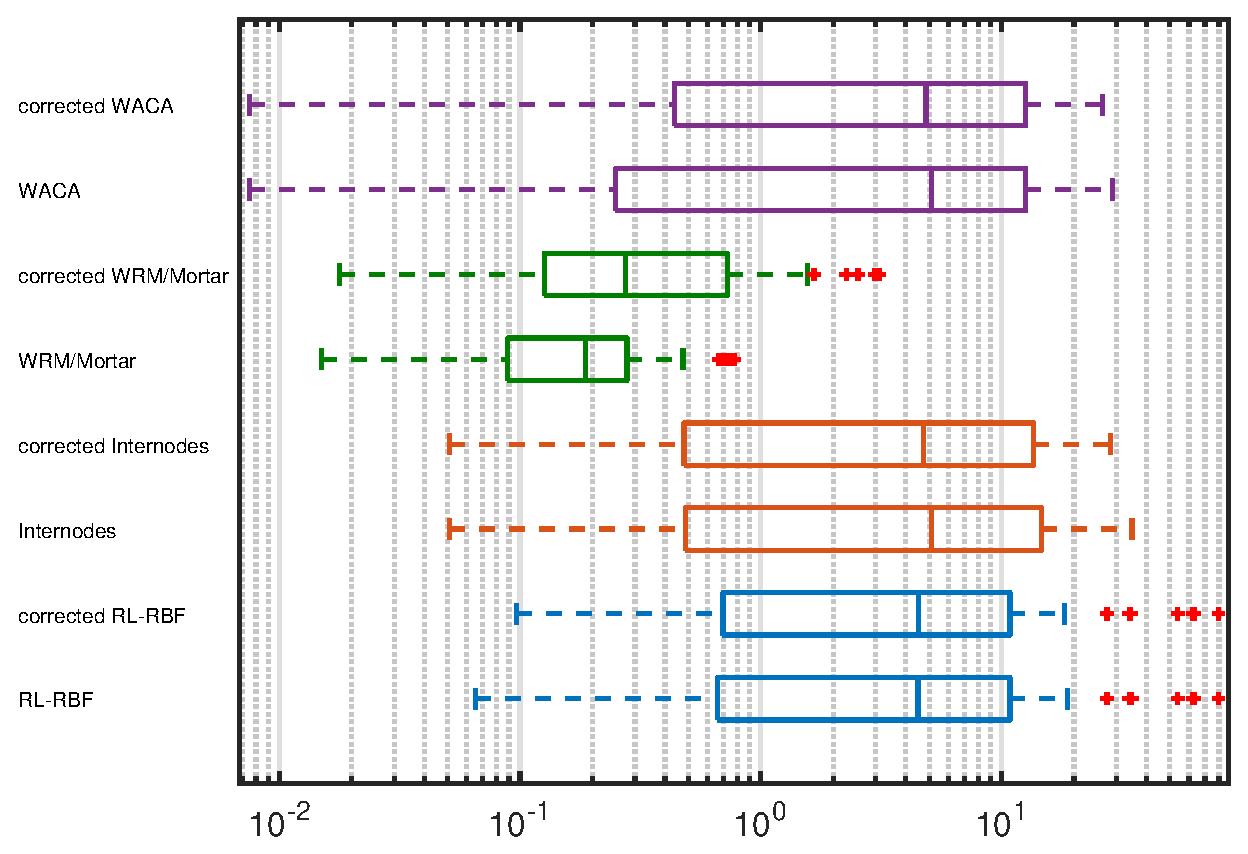
\includegraphics[width=0.7\linewidth]{images/Ch1/boxplot_EK}
 \caption{Boxplot of $E_K$, interface kinetic energy relative error.\label{fig.30}}
 \label{fig:boxplot_EK}
 \end{figure}
 
 Figure \ref{fig.30} results of all previous experiences are given also for $E_K \%$. We can see from these boxplots that further developments are still possible aimed at improving specifically the accuracy of the methods for dynamic problems.
\section{Advanced solver for FEA}
\subsection{Superelement exploitation}
\label{subsection1.4.1}
In the previous sections a 3D solid finite element formulation was considered. These, even if very general, suffer of strong limitations, when considering degenerated geometry, such as beam or shell geometries. In such structures linear solid elements suffer of some important shortcomings such as shear locking or computational burden. For this reason more specific component such as beam or shell elements have been developed in many FEM libraries. The Whole Engine Model (WEM) in our context is a very complex assembly of many different kinds of Elements, with many complicated loadings computed from both the engine manufacturer and the load analysis department. In such way of working the WEM needs to be considered with its contributions to loads and stiffness. These two contribute to the final measure of engine displacements that we want to monitor in this study.  The fact that an industrial engine model has to be integrated in the finite element analysis poses a real problem in terms of both implementation efficiency and development time since the combined engine and design zone structural model may be too complex and computationally expensive to be solved at each iteration of the optimization process. To circumvent these issues superelements \cite{nastran2013superelements} were employed. These are very efficient to deal with complex linear models that do not change in the optimization loop \cite{krog2004topology}.
Here we develop this method on a general structure shown in Figure \ref{f.3}.
\begin{figure}[hbt!]
\centering
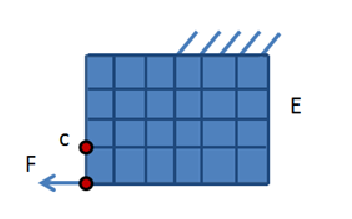
\includegraphics[width=.4\textwidth]{images/Ch1/dof_part.eps}
\caption{Example of DOFs partition: the nodes of the structure are sorted in retained nodes (whose DOFs are ($c$)) and other nodes (whose  DOFs are ($E$)). After the static condensation, a superelement containing only ($c$) DOFs will be generated. Nevertheless the suppressed DOFs ($E$) can still be computed after static analysis thanks to equation \ref{e.7}.  \label{f.3}}
\end{figure}
Sorting the structure's degrees of freedom into retained ($c$) and other degrees of freedom ($E$)\footnote{note that here ($E$) indicates only free DOFs and homogeneous Dirichlet conditions are considered.}, the static balance equation can then be written in the following form:
\begin{equation}
\label{e.6}
\left[ \begin{array}{cc}
\left[ \mathbf{K_{cc}} \right] & \left[ \mathbf{K_{cE}} \right]\\
\left[ \mathbf{K_{Ec}} \right] & \left[ \mathbf{K_{EE}} \right]
\end{array} \right] \left\lbrace \begin{array}{c}
\lbrace u_c \rbrace\\
\lbrace u_E \rbrace\\
\end{array}\right\rbrace =  \left\lbrace \begin{array}{c}
\lbrace F_c \rbrace\\
\lbrace F_E \rbrace\\
\end{array}\right\rbrace
\end{equation}
Using the second line block of equations and solving for $\lbrace u_E \rbrace$
\begin{equation}
\label{e.7}
\lbrace u_E \rbrace =\left[ P \right]\lbrace u_c \rbrace + \lbrace u_0 \rbrace
\end{equation}
With 
\begin{eqnarray}
\left[P\right]=-\left[ \mathbf{K_{EE}}\right]^{-1} \left[\mathbf{K_{Ec}}\right] \\
\lbrace u_0 \rbrace=\left[\mathbf{K_{EE}}\right]^{-1}\lbrace F_E \rbrace
\end{eqnarray}
The $\left[P\right]$ matrix is called constrained modal matrix in Nastran and recovery matrix in Abaqus. $\lbrace u_0 \rbrace$ is called fixed interface displacement on Nastran and has to be computed in a separated analysis on Abaqus.
Substituting   equation \ref{e.7} back in the first line block of \ref{e.6}:
\begin{equation}
\label{e.10}
\left[ \mathbf{\tilde{K}_{cc}}\right]\lbrace u_c \rbrace=\lbrace \tilde{F}_c \rbrace 
\end{equation}
With 
\begin{eqnarray}
\left[ \mathbf{\tilde{K}_{cc}}\right]=\left[\mathbf{K_{cc}}\right]+ \left[ P\right]^T\left[ \mathbf{K_{Ec}}\right] \\
\lbrace \tilde{F}_c \rbrace =\lbrace F_c \rbrace + \left[ P\right]^T\lbrace F_E \rbrace
\end{eqnarray}
In our problem we can make the evaluation of $ \left[ \mathbf{\tilde{K}_{cc}}\right]$ ,$\lbrace \tilde{F}_c \rbrace$ , $\left[ P\right]$ using a commercial software like Abaqus using the engine model. 
The $\lbrace u_0 \rbrace$ vector can also be evaluated using a linear perturbation static analysis of the engine, fixing the DOFs of the interface. If the structure has to be integrated into another model, the retained DOFs ($c$) can be used to describe the displacements of the whole assembly. The stiffness matrix of equation \ref{e.6} doesn't need to be inverted anymore, the only knowledge of $\left[\mathbf{\tilde{K}_{cc}}\right]$ and $\lbrace \tilde{F}_c \rbrace$ is sufficient.
Considering the engine interface DOFs as retained DOFs ($c$), we can make possible the evaluation of engine and design zone assembly displacements just considering the retained DOFs stiffness matrix and load vector. Using mesh tying techniques reviewed in section \ref{sec1.3} the engine retained nodes stiffness matrix and load vector can be integrated to the design zone.
In fact let's consider a simple elimination approach for the mesh tying of engine superelement and design zone finite element model.
  \begin{equation}
    \lbrace u_c \rbrace = \left[ \Pi_{cd} \right] \lbrace u_{d}\rbrace
    \end{equation}
Where $\lbrace u_c \rbrace$, $\lbrace u_{d}\rbrace $ are respectively engine and design zone interface DOFs.
After eliminating engine DOFs, the final system of equation reads :
    \begin{equation}
    \label{eq.1.119}
    \left[ \begin{array}{cc}
    \left[ \mathbf{K_{oo}} \right] & \left[ \mathbf{K_{od}} \right]\\
    \left[ \mathbf{K_{do}} \right] & \left[ \mathbf{K_{dd}} \right]+\left[ \Pi_{cd} \right]^T\left[ \mathbf{\tilde{K}_{cc}} \right]\left[ \Pi_{cd} \right]
    \end{array} \right] \left\lbrace \begin{array}{c}
    \lbrace u_o \rbrace\\
    \lbrace u_d \rbrace\\
    \end{array}\right\rbrace =  \left\lbrace \begin{array}{c}
    \lbrace F_o \rbrace\\
    \lbrace F_d\rbrace+\left[ \Pi_{cd} \right]^T\lbrace \tilde{F}_c\rbrace\\
    \end{array}\right\rbrace
    \end{equation} 
Where $o$ is the index of design zone DOFs not lying on the interface and:
\begin{equation}
\MatrixVar{\mathbf{K_{DZ}}}=\left[ \begin{array}{cc}
    \left[ \mathbf{K_{oo}} \right] & \left[ \mathbf{K_{od}} \right]\\
    \left[ \mathbf{K_{do}} \right] & \left[ \mathbf{K_{dd}} \right] 
    \end{array} \right] 
\end{equation}
Is the stiffness matrix relative to the Design Zone of the topology optimization problem and
\begin{equation}
\MatrixVar{\mathbf{K_{Eng}}}=\left[ \begin{array}{cc}
    \left[ 0 \right] & \left[ 0 \right]\\
    \left[ 0 \right] & \left[ \Pi_{cd} \right]^T\left[ \mathbf{\tilde{K}_{cc}} \right]\left[ \Pi_{cd} \right] 
    \end{array} \right] 
\end{equation} 
Is the engine superelement stiffness matrix.
The final system of equations in this case can then be written in a short form as :
\begin{equation}
\left(\MatrixVar{\mathbf{K_{Eng}}}+\MatrixVar{\mathbf{K_{DZ}}}\right)\VectorVar{U}=\MatrixVar{\mathbf{K}}\VectorVar{U}=\VectorVar{F}
\end{equation}
The superelement exploitation implies a significant economy in CPU time especially for big and complex engine models, since the full engine model does not have to be evaluated at each change of the design zone considered by the topology optimization. Furthermore, this also implies that the software used for evaluating the engine model can be separate from the one for evaluating the design zone model and carrying out the topology optimization. This is important since in practice the engine model is usually constructed in commercial FE software. In this work we used Abaqus for the engine model and Matlab for the design zone model and topology optimization. Accordingly reading Abaqus \textit{.dat} and \textit{.mtx} file from Matlab environment we can make the evaluation of the whole structure just using the Matlab environment as is summarized in figure \ref{f.6b}. Abaqus is used to generate both the engine and the design zone. A parsing of the input file is made on Matlab to import the design zone mesh coordinates and finite elements. The engine model is reduced to a superelement on the interface using Abaqus, then a parsing is made on the .mtx and the .dat file coming respectively from the sub-structuring and the linear load case. 
The stiffness matrix of the design zone is assembled together with the engine superelement stiffness matrix, the same is done for the load vectors. For each iteration of the topology optimization loop, the assembled problem is solved to determine the design zone displacements and the recovered engine displacements.  Finally tip clearance variations are computed in each stage and employed to compute consumption variation.
\begin{figure}[hbt!]
\centering
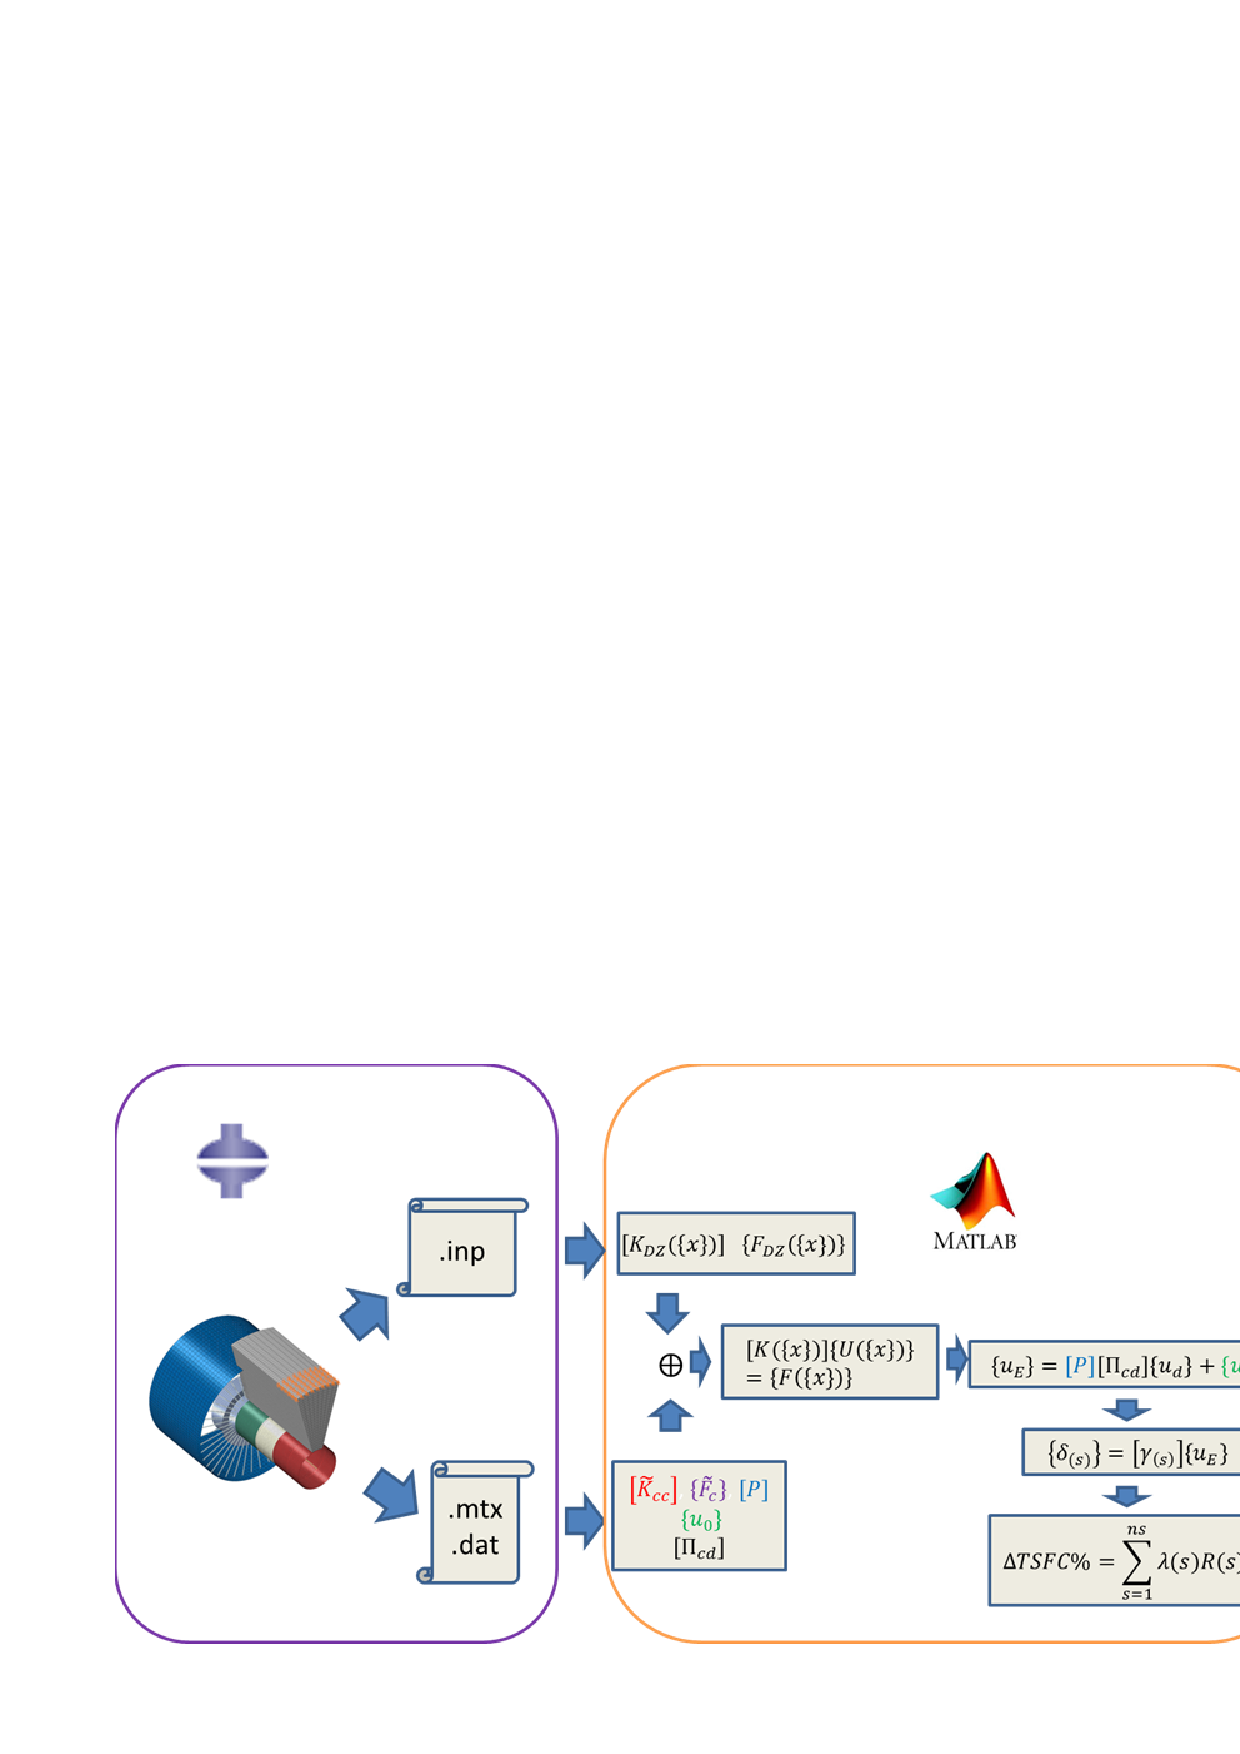
\includegraphics[width=0.85\textwidth]{images/Ch1/tip_cl_wkf.png}
\caption{Tip-clearance evaluation work-flow. 
\label{f.6b}}
\end{figure}
 This gives significant flexibility in implementing various approaches developed for topology optimization.
\subsection{Iterative solvers}
\label{subsection1.4.2}
Solving the balance equations \eqref{eq.1.119} for the free DOFs vector is an expensive task especially for large 3D problem as the one we try to tackle in this work. The stiffness matrix is large, sparse and positive definite. For this reason one can either employ direct solvers \cite{davis2006direct} or
iterative solvers \cite{saad2003iterative}. When dealing with small 2D problems, direct solvers are preferable due to their computational efficiency and robustness. In these approaches, the stiffness matrix is decomposed in the product of a lower triangular and an upper triangular matrices (LU or Choleski decompositions). Then, the resolution two systems of linear equations is carried out as a back substitution operation. For large scale 3D problems, these approaches become too expensive and ineffective \cite{davis2006direct}. For these cases, the sparsity of the stiffness matrix results in an inexpensive matrix vector product operation which can be effectively utilized by iterative solution algorithms.
\subsubsection{The Conjugate Gradient Algorithm}
 For symmetric positive definite matrices, a classic choice in terms of iterative solvers is the Conjugate Gradient (CG) algorithm \cite{hestenes1952methods}. Here we derive this algorithm following the procedure illustrated in \cite{saad2003iterative}. At each iteration $k$ of the Conjugate Gradient algorithm, the solution vector $\VectorVar{U}$ is updated as:
\begin{equation}
\VectorVar{U}_{(k+1)}=\VectorVar{U}_{(k)}+\alpha_{(k)}\VectorVar{p}_{(k)}
\end{equation}
where $\VectorVar{U}_{(k+1)}$ is the solution at the next iteration $k+1$ that is written in function of the solution at the previous iteration $\VectorVar{U}_{(k)}$, $\alpha_{(k)}$ is a scalar and $\VectorVar{p}_{(k)}$ is the perturbation direction at the same iteration $k$. One can define the residual vector $\VectorVar{r}$ defined at each iteration as:
\begin{equation}
\VectorVar{r}_{(k)}=\VectorVar{F}-\MatrixVar{\mathbf{K}}\VectorVar{U}_{(k)}
\end{equation}
The residual for the $k+1$ iteration can be then written as:
\begin{equation}
\VectorVar{r}_{(k+1)}=\VectorVar{F}-\MatrixVar{\mathbf{K}}\VectorVar{U}_{(k)}-\alpha_{(k)}\MatrixVar{\mathbf{K}}\VectorVar{p}_{(k)}=\VectorVar{r}_{(k)}-\alpha_{(k)}\MatrixVar{\mathbf{K}}\VectorVar{p}_{(k)}
\end{equation}
To enforce the residual at the iteration $k+1$ to be orthogonal to the one of the previous iteration $k$:
\begin{equation}
\VectorVar{r}_{(k+1)}^T \VectorVar{r}_{(k)}=0
\end{equation}
That is true only if:
\begin{equation}
\alpha_{(k)}=\frac{\VectorVar{r}_{(k)}^T\VectorVar{r}_{(k)}}{\VectorVar{r}_{(k)}^T\MatrixVar{\mathbf{K}}\VectorVar{p}_{(k)}}
\end{equation}
For the update of the search direction, one can ask that it has to belong to the span of vectors $\VectorVar{r}_{(k+1)}$ and $\VectorVar{p}_{(k)}$:
\begin{equation}
\label{eq.1.128}
\VectorVar{p}_{(k+1)}=\VectorVar{r}_{(k+1)} +\beta_{(k)}\VectorVar{p}_{(k)}
\end{equation}
To determine $\beta_{(k)}$ one has to enforce this time the orthogonality between $\VectorVar{p}_{(k+1)}$ and $\MatrixVar{\mathbf{K}}\VectorVar{p}_{(k)}$:
\begin{equation}
\label{eq.1.129}
\VectorVar{p}_{(k)}^T\MatrixVar{\mathbf{K}}\VectorVar{p}_{(k+1)}=0
\end{equation}
true only if:
\begin{equation}
\beta_{(k)}=-\frac{\VectorVar{p}_{(k)}^T\MatrixVar{\mathbf{K}}\VectorVar{r}_{(k+1)}}{\VectorVar{p}_{(k)}^T\MatrixVar{\mathbf{K}}\VectorVar{p}_{(k)}}
\end{equation}
Being:
\begin{equation}
\MatrixVar{\mathbf{K}}\VectorVar{p}_{(k)}=-\frac{1}{\alpha_{(k)}}\left(\VectorVar{r}_{(k+1)}-\VectorVar{r}_{(k)}\right)
\end{equation}
So that:
\begin{equation}
\beta_{(k)}=\frac{\VectorVar{r}_{(k+1)}^T\VectorVar{r}_{(k+1)}}{\alpha_{(k)}\VectorVar{p}_{(k)}^T\MatrixVar{\mathbf{K}}\VectorVar{p}_{(k)}}
\end{equation}
Using equations \eqref{eq.1.128} and \eqref{eq.1.129}:
\begin{equation}
\VectorVar{p}_{(k)}^T\MatrixVar{\mathbf{K}}\VectorVar{p}_{(k)}=\VectorVar{p}_{(k)}^T\MatrixVar{\mathbf{K}}\left(\VectorVar{r}_{(k)} +\beta_{(k-1)}\VectorVar{p}_{(k-1)}\right)=\VectorVar{p}_{(k)}^T\MatrixVar{\mathbf{K}}\VectorVar{r}_{(k)}
\end{equation}
then:
\begin{equation}
\beta_{(k)}=\frac{\VectorVar{r}_{(k+1)}^T\VectorVar{r}_{(k+1)}}{\VectorVar{r}_{(k)}^T\VectorVar{r}_{(k)}}
\end{equation}
The CG algorithm can then be written as:
\begin{algorithm}
\KwIn{$\MatrixVar{\mathbf{K}},\VectorVar{F},\varepsilon_{U}, N_{max}$}
\KwOut{$\VectorVar{U}_{(k)}$ approximation of the solution of $\MatrixVar{\mathbf{K}}\VectorVar{U}=\VectorVar{F}$ }

$k\gets 0$\;
$\VectorVar{U}_{(0)}\gets\VectorVar{0}$\;
$\VectorVar{r}_{(0)}\gets \VectorVar{F}$\;
$\VectorVar{p}_{(0)}\gets \VectorVar{r}_{(0)}$\;
 \While{$\frac{\|\VectorVar{r}_{(k)}\|_2}{\|\VectorVar{r}_{(0)}\|_2}\leq \varepsilon_{r}$ or $k\geq N_{max}$}{
 $\alpha_{(k)}\gets\frac{\VectorVar{r}_{(k)}^T\VectorVar{r}_{(k)}}{\VectorVar{p}_{(k)}^T\MatrixVar{\mathbf{K}}\VectorVar{p}_{(k)}}$\;
 $\VectorVar{U}_{(k+1)}\gets\VectorVar{U}_{(k)}+\alpha_{(k)}\VectorVar{p}_{(k)}$\;
$\VectorVar{r}_{(k+1)}\gets\VectorVar{r}_{(k)}-\alpha_{(k)}\MatrixVar{\mathbf{K}}\VectorVar{p}_{(k)}$\;
$\beta_{(k)}\gets\frac{\VectorVar{r}_{(k+1)}^T\VectorVar{r}_{(k+1)}}{\VectorVar{r}_{(k)}^T\VectorVar{r}_{(k)}}$\;
$\VectorVar{p}_{(k+1)}\gets\VectorVar{r}_{(k+1)} +\beta_{(k)}\VectorVar{p}_{(k)}$\;
  $k\gets k+1$\;
 }
 \KwRet{$\VectorVar{U}_{(k)}$}
 \caption{Conjugate Gradient \label{CG}}
\end{algorithm}
\subsubsection{The Preconditioned Conjugate Gradient (PCG) Algorithm}
It can be proven \cite{saad2003iterative} that CG reaches the solution vector $\VectorVar{U^*}$ in at most $n$ iterations\footnote{$n$ being the number of free DOFs i.e. the length of $\VectorVar{F}$.},and the convergence rate is shown to be:
\begin{equation}
\label{eq.1.135}
\|\VectorVar{U}_{(k)}-\VectorVar{U^*}\|_{\MatrixVar{\mathbf{K}}}\leq 2 \left(\frac{\sqrt{\kappa}-1}{\sqrt{\kappa}+1}\right)^k\|\VectorVar{U}_{0}-\VectorVar{U^*}\|_{\MatrixVar{\mathbf{K}}}
\end{equation}
where the $\MatrixVar{\mathbf{K}}$-norm of a vector is defined as:
\begin{equation}
\|\VectorVar{x}\|_{\MatrixVar{\mathbf{K}}}=\sqrt{\VectorVar{x}\MatrixVar{\mathbf{K}}\VectorVar{x}}
\end{equation}
$k$ is the iteration where the CG algorithm was stopped and $\kappa$ is the condition number of the stiffness matrix $\MatrixVar{\mathbf{K}}$. Equation \eqref{eq.1.135} shows that for $\kappa\gg 1$ the convergence of CG algorithm is very slow. In practice to accelerate and ensure convergence, preconditioning techniques are employed. The basic idea of these techniques is to replace the original system of equations by another one that has the same solution and is easier to be solved by iterative algorithms. An operator $\MatrixVar{\mathbf{M}}^{-1}$ has to be constructed so that $\kappa(\MatrixVar{\mathbf{M}}^{-1}\MatrixVar{\mathbf{K}}) \ll \kappa( \MatrixVar{\mathbf{K}})$.
By the use of such techniques the CG algorithm can be modified as in algorithm \ref{PCG}.
\begin{algorithm}[ht!]
\KwIn{$\MatrixVar{\mathbf{K}},\MatrixVar{\mathbf{M}}^{-1},\VectorVar{F},\varepsilon_{U}, N_{max}$}
\KwOut{$\VectorVar{U}_{(k)}$ approximation of the solution of $\MatrixVar{\mathbf{K}}\VectorVar{U}=\VectorVar{F}$ }

$k\gets 0$\;
$\VectorVar{U}_{(0)}\gets\VectorVar{0}$\;
$\VectorVar{r}_{(0)}\gets \VectorVar{F}$\;
$\VectorVar{z}_{(0)}\gets \MatrixVar{\mathbf{M}}^{-1} \VectorVar{r}_{(0)}$\;
$\VectorVar{p}_{(0)}\gets \VectorVar{z}_{(0)}$\;
 \While{$\frac{\|\VectorVar{r}_{(k)}\|_2}{\|\VectorVar{r}_{(0)}\|_2}\leq \varepsilon_{r}$ or $k\geq N_{max}$}{
 $\alpha_{(k)}\gets\frac{\VectorVar{r}_{(k)}^T\VectorVar{z}_{(k)}}{\VectorVar{p}_{(k)}^T\MatrixVar{\mathbf{K}}\VectorVar{p}_{(k)}}$\;
 $\VectorVar{U}_{(k+1)}\gets\VectorVar{U}_{(k)}+\alpha_{(k)}\VectorVar{p}_{(k)}$\;
$\VectorVar{r}_{(k+1)}\gets\VectorVar{r}_{(k)}-\alpha_{(k)}\MatrixVar{\mathbf{K}}\VectorVar{p}_{(k)}$\;
$\VectorVar{z}_{(k+1)}\gets\MatrixVar{\mathbf{M}}^{-1} \VectorVar{r}_{(k+1)}$\;
$\beta_{(k)}\gets\frac{\VectorVar{z}_{(k+1)}^T\VectorVar{r}_{(k+1)}}{\VectorVar{z}_{(k)}^T\VectorVar{r}_{(k)}}$\;
$\VectorVar{p}_{(k+1)}\gets\VectorVar{z}_{(k+1)} +\beta_{(k)}\VectorVar{p}_{(k)}$\;
  $k\gets k+1$\;
 }
 \KwRet{$\VectorVar{U}_{(k)}$}
 \caption{Preconditioned Conjugate Gradient \label{PCG}}
\end{algorithm}
One can observe that the application of the projection operator in \ref{PCG}, is needed once per iteration. For this reason a good preconditioning operator should be:
\begin{itemize}
\item Cheap: its application should not involve too many operations
\item Effective: $\kappa(\MatrixVar{\mathbf{M}}^{-1}\MatrixVar{\mathbf{K}})$ should be as close as possible to 1.
\item Scalable:  $\kappa(\MatrixVar{\mathbf{M}}^{-1}\MatrixVar{\mathbf{K}})$ and its computational burden should be proportional to the problem size $n$.
\item Robust:  $\MatrixVar{\mathbf{M}}^{-1}$ efficiency should not be problem dependent.
\item Simple:  complexity should be justified by the computational gain.
\end{itemize}
Among most common general purpose techniques we can find incomplete Cholesky Factorization \cite{kershaw1978incomplete}, the diagonal compensation \cite{jacobi1845ueber} and the Factorized Sparse Approximate Inverses (FSAI) \cite{buleev1960numerical,buleev1960numerical2,meijerink1977iterative,il1992iterative,varga1960boundary}. All these techniques are well adapted when the matrix of coefficients is not linked with a particular physics. In the next subsection we describe multi-grid approaches that take advantage from the fact that the matrix of coefficients comes from a PDE problem discretization.
\subsubsection{Multigrid Methods}
\label{multigrid}
The convergence of PCG for solving linear systems arising from PDE slows down with the size of the problem. Multigrid methods \cite{trottenberg2001multigrid} have been initially designed specifically to solve such problems. On the other hands these approaches' success is strongly dependent on the problem at hand and they need attention to get improved performances. They consist in the use of smoothers and coarse level corrections. 
Considering the residual decomposition over the basis of eigenvectors of the stiffness matrix, it can be shown that residual components associated with higher frequencies, are damped within few iterations by simple smoothing techniques like damped Jacobi, Gauss Seidel or Red-Black Gauss Seidel \cite{saad2003iterative}. On the other hand the low frequency components survive the smoothing step and need to be dealt with by coarse mesh corrections. The proofs of this results can be found in \cite{saad2003iterative}, for uniform 1D and 2D discretizations. In the present work we considered non uniform meshes, and this can be challenging for theoretical reasons, since one cannot directly transpose the considerations valid for uniform meshes to non-uniforms ones, and for practical reasons, since prolongation and interpolation operators may not be easily available. For this reason in the literature one can find Algebraic Multigrid (AMG) \cite{stuben2001review} that tries to emulate Geometric Multigrid (GMG) performance on the only knowledge of the coefficient matrix. In this work we focus our analysis on hierarchical non uniform hexahedral meshes.  This means that we considered fine meshes to be a consequence of a coarse mesh successive refinements. Each mesh refinement is considered as a level in the GMG.
In this way it is relatively simple to construct Interpolation and Prolongation operators to transfer vectors through levels.
Given a finite element of the coarse mesh, its refinement can be obtained cutting each finite element in 8 as shown in figures
\ref{f7},\ref{f8}.  
  \begin{figure}[hbt!]
  \centering
       \subfloat[ \label{fig.7a}]{%
                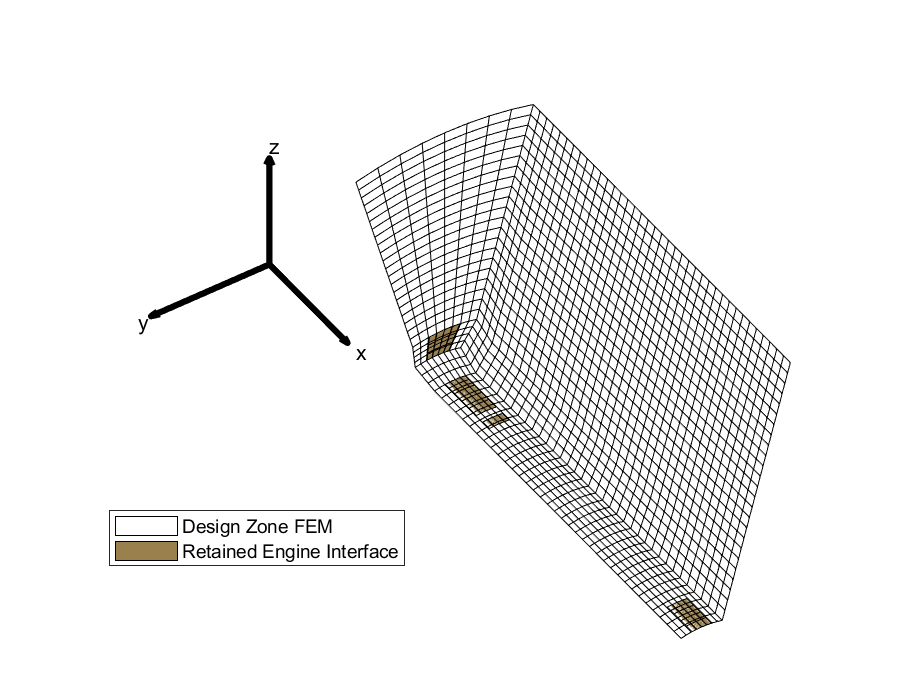
\includegraphics[width=0.5\textwidth]{images/Ch1/original_mesh.eps}
              }
       \subfloat[  \label{fig7b}]{%
         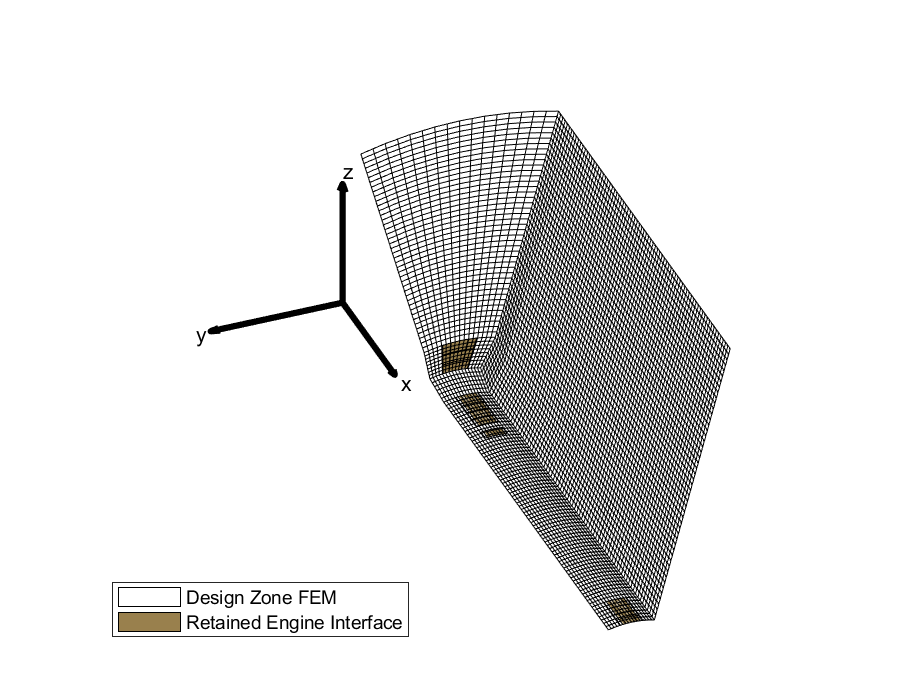
\includegraphics[width=0.5\textwidth]{images/Ch1/mesh_ref1.eps}
       }
       \caption{Mesh refinement procedure needed for multi-grid approach. The engine reduced element set is colored in yellow. Each node of these elements is kept in the engine superelement.(a) Original design zone mesh, generated in Abaqus and imported on matlab by input file parsing. The mesh counts 7600 8-node linear 3D solid finite elements and 9126 nodes. (b) Design zone mesh after refinement. Each element of the original element is cut in 8 new elements, that give a total of 7600$\times$8=60800 8-node linear 3D solid finite elements and  66759 nodes. }
       \label{f7}
     \end{figure} 
    \begin{figure}[hbt!]
        \centering
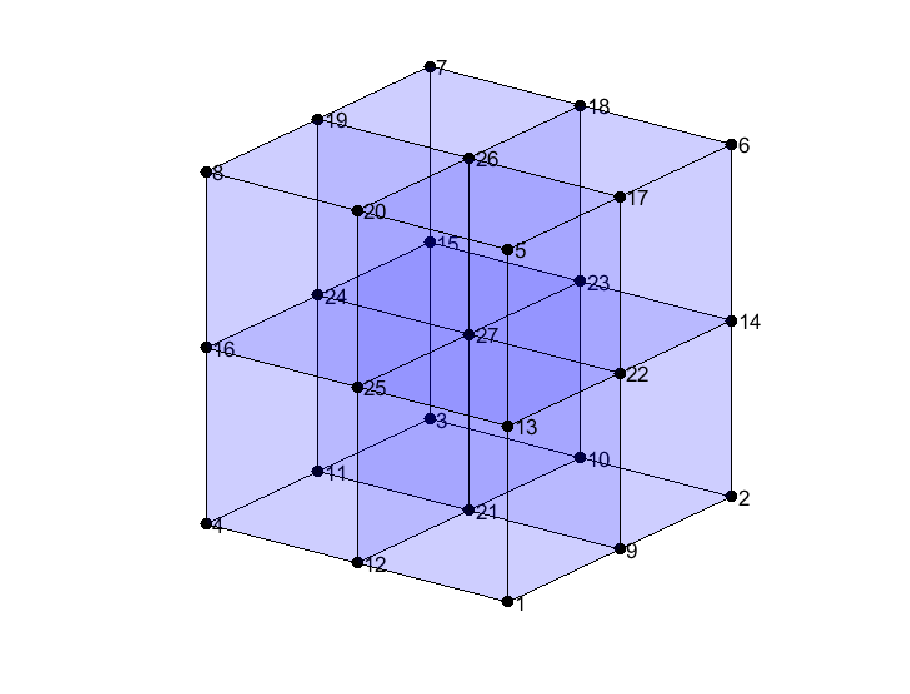
\includegraphics[width=0.5\textwidth]{images/Ch1/partition_3D.eps}
  \caption{3D partition employed for mesh refinement, nodes 1 to 8 belong to original coarse mesh element. Partition determines node 9 to 27 and 8 elements of the finer mesh.  }
       \label{f8}
     \end{figure}
     For each element of the coarse mesh we can define a transfer of the information between coarse level filed $u^c_i$ $i=1,2,...,8$ and the fine level field $u^f_j$ $j=1,2,...,27$, that can be used to construct the interpolation operator. 
     \begin{itemize}
     \item Node 1 to 8 of the fine mesh have their corresponding node in the coarse level so that: $u^c_i=u^f_i$ for $i=1,2,...,8$.
     \item Nodes 9 to 20 are in the middle of a coarse element edge. For this reason their field can be interpolated using the extremities of edges. For example $u^f_9=\frac{u^c_1+u^c_2}{2}$.
     \item Nodes 21 to 26 correspond to coarse element facet middle points. The corresponding component can be interpolated by the vertex of the corresponding coarse element facets. For instance $u^f_{21}=\frac{u^c_1+u^c_2+u^c_5+u^c_6}{4}$.
     \item Finally node 27 is in the coarse element centroid. Its nodal variable can be interpolated using all the coarse mesh node variables: $u^f_{27}=\frac{u^c_1+u^c_2+u^c_3+u^c_4+u^c_5+u^c_6+u^c_7+u^c_8}{8}$.
     \end{itemize}
        All previous relationships can be written in the matrix form: 
     \begin{equation}
     \VectorVar{u_f^{el}}=\MatrixVar{I_{fc}^{el}}\VectorVar{u_c^{el}}
     \end{equation}
     When considering the communication of several independent fields between each level one can use the same interpolation operator for each field:
     \begin{equation}
     \VectorVar{U_f^{el}}=\MatrixVar{I_{fc}^{el}\bigotimes I_d}\VectorVar{U_c^{el}}
     \end{equation}
     where $\bigotimes$ denotes the Kronecker product.
     Finally one can combine the equations coming from each coarse level element to build the global Interpolation operator. In doing so one has to consider each DOF of the fine mesh only once. Generally speaking the interpolation between the $l^{th}$ refinement and the corresponding coarser level is given by: 
      \begin{equation}
      \VectorVar{U_l}=\MatrixVar{I_{l,l-1}}\VectorVar{U_{l-1}}
      \end{equation}
      The prolongation operator allows for the inverse communication.  
 \begin{equation}
       \VectorVar{U_{l-1}}=\MatrixVar{P_{l-1,l}}\VectorVar{U_{l}}
 \end{equation}
 To keep the stiffness matrix at each refinement symmetric, the prolongation operator is considered to be:
 \begin{equation}
 \MatrixVar{P_{l-1,l}}=\MatrixVar{I_{l,l-1}}^T
 \end{equation}
 In this way given the state problem at the l-th refinement:
 \begin{equation}
 \MatrixVar{\mathbf{K_{l}}}\VectorVar{U_{l}}=\VectorVar{F_{l}}
 \end{equation}
 one can get a state problem at the coarser level as:
  \begin{equation}
  \MatrixVar{I_{l,l-1}}^T \MatrixVar{\mathbf{K_{l}}}\MatrixVar{I_{l,l-1}}\VectorVar{U_{l-1}}=\MatrixVar{\mathbf{K_{l-1}}}\VectorVar{U_{l-1}}=\MatrixVar{I_{l,l-1}}^T\VectorVar{F_{l}}=\VectorVar{F_{l-1}}
  \end{equation}
  This notation will be used to define the coarse mesh correction step needed in the multigrid. The other important ingredient plays a fundamental role in multigrid convergence is the smoothing.
  Here we will note:
  \begin{equation}
 \VectorVar{U_{l,\upsilon}}=\textit{smooth}^{\upsilon}(\MatrixVar{\mathbf{K_{l}}},\VectorVar{U_{l,0}},\VectorVar{F_{l}})
  \end{equation}
  where $\textit{smooth}^{\upsilon}$ denotes the application of $\upsilon$ steps of the form:
  \begin{equation}
 \VectorVar{ U_{l,j+1}}= \MatrixVar{\mathbf{B_{l}}}\VectorVar{U_{l,j}}+\MatrixVar{\mathbf{C_{l}}}\left(\VectorVar{F_{l}}\right)
  \end{equation}
  Where the matrix $\MatrixVar{\mathbf{B_{l}}}$ and $\MatrixVar{\mathbf{C_{l}}}$ depend on the particular approach chosen for the smoothing and will be detailed later. For two levels the multigrid algorithm can be encoded as in algorithm \ref{TGC}.
  \begin{algorithm}
 Pre-smooth: $\VectorVar{U_{l}}\gets\textit{smooth}^{\upsilon_1}(\MatrixVar{\mathbf{K_{l}}},\VectorVar{U_{l}},\VectorVar{F_{l}})$\;
 Get residual: $\VectorVar{r_{l}}\gets\VectorVar{F_{l}}-\MatrixVar{\mathbf{K_{l}}}\VectorVar{U_{l}}$\;
 Coarsen: $\VectorVar{r_{l-1}}\gets\MatrixVar{I_{l,l-1}}^T\VectorVar{r_{l}}$\;
 Solve: $\MatrixVar{\mathbf{K_{l-1}}}\VectorVar{\delta_{l-1}}=\VectorVar{r_{l-1}}$\;
 Correct: $\VectorVar{U_{l}}\gets\VectorVar{U_{l}}+\MatrixVar{I_{l,l-1}}\VectorVar{\delta_{l-1}}$\;
 Post-smooth: $\VectorVar{U_{l}}\gets\textit{smooth}^{\upsilon_2}(\MatrixVar{\mathbf{K_{l}}},\VectorVar{U_{l}},\VectorVar{F_{l}})$\;
   \caption{Two Grid cycle \label{TGC}}
  \end{algorithm}
Note that using this technique recursively, the algorithm moves to coarsen levels until the coarsest mesh is reached and direct solvers can indeed be employed to solve the corresponding state problem. Such idea is at the origin of the V-cycle (c.f. algorithm \ref{Vcy}).
  \begin{algorithm}
 Pre-smooth: $\VectorVar{U_{l}}\gets\textit{smooth}^{\upsilon_1}(\MatrixVar{\mathbf{K_{l}}},\VectorVar{U_{l}},\VectorVar{F_{l}})$\;
 Get residual: $\VectorVar{r_{l}}\gets\VectorVar{F_{l}}-\MatrixVar{\mathbf{K_{l}}}\VectorVar{U_{l}}$\;
 Coarsen: $\VectorVar{r_{l-1}}\gets\MatrixVar{I_{l,l-1}}^T\VectorVar{r_{l}}$\;
If $l=1$\;
 Solve: $\MatrixVar{\mathbf{K_{l-1}}}\VectorVar{\delta_{l-1}}=\VectorVar{r_{l-1}}$\;
 Else \;
 Recursion: $\VectorVar{\delta_{l-1}}\gets$V-cycle$(\MatrixVar{\mathbf{K_{l-1}}},\VectorVar{0},\VectorVar{r_{l-1}})$\;
End \;
 Correct: $\VectorVar{U_{l}}\gets\VectorVar{U_{l}}+\MatrixVar{I_{l,l-1}}\VectorVar{\delta_{l-1}}$\;
 Post-smooth: $\VectorVar{U_{l}}\gets\textit{smooth}^{\upsilon_2}(\MatrixVar{\mathbf{K_{l}}},\VectorVar{U_{l,0}},\VectorVar{F_{l}})$\;
   \caption{$\VectorVar{U_{l}}$=V-cycle$(\MatrixVar{\mathbf{K_{l}}},\VectorVar{U_{l}},\VectorVar{F_{l}})$ \label{Vcy}}
  \end{algorithm}
  One can observe that in the V-cycle only matrix times vector multiplications are introduced at each prolongation and interpolation step. This operator can be introduced in line 10 of PCG \ref{PCG}. The resulting algorithm also called Multigrid Conjugate Gradients) (MGCG) \cite{tatebe1994efficient,ashby1996parallel} depending on the smoother and the number of levels can be both robust and efficient for solving the linear system associated with the displacement evaluation in topology optimization \cite{amir2014multigrid,aage2017giga}. As aforementioned, the smother choice has to be complementary to the coarse mesh corrections in terms of residual error components. In the problem at hand, superelements and non-uniform meshes make this choice particularly important. Damped Jacobi iterations (c.f. \ref{DJs}) are inexpensive and effective options especially for large problems.
  \begin{algorithm}
 $\VectorVar{U_{l}}\gets\VectorVar{U_{l}}+\omega\MatrixVar{\mathbf{D_{l}}}^{-1}\left(\VectorVar{F_{l}}-\MatrixVar{\mathbf{K_{l}}}\VectorVar{U_{l}}\right)$\;
 \caption{Damped Jacobi smoother \label{DJs}}
  \end{algorithm}
  \clearpage
  Where $\MatrixVar{\mathbf{D_{l}}}$ is the diagonal matrix of $\MatrixVar{\mathbf{K_{l}}}$. 
   On the other hand bad mesh quality and static condensation can cause large positive out-of-diagonal terms in the final stiffness matrix that can make diagonal scaling ineffective. Another issue consists in the choice of the damping parameter $\omega$. Theoretical considerations can be applied for the uniform meshes as explained in \cite{saad2003iterative}. For non-uniform meshes and for superelements, the accurate choice of this parameter can be even more complicated \cite{bin2010geometric}.
   We can cite here other effective smoother techniques that can be employed instead of damped Jacobi iterations.
   The  multi-parameter Jacobi method that can be considered as the sequential application of Jacobi step with different values (c.f. algorithm \ref{MPJ}).
     \begin{algorithm}
     For $j=1,2,...,p$\;
    $\VectorVar{U_{l}}\gets\VectorVar{U_{l}}+\omega_j\MatrixVar{\mathbf{D_{l}}}^{-1}\left(\VectorVar{F_{l}}-\MatrixVar{\mathbf{K_{l}}}\VectorVar{U_{l}}\right)$\;
    End\;
    \caption{Multi-parameter Jacobi Method \label{MPJ}}
     \end{algorithm}
  Using such approach, the frequency range on which damping is effective can be amplified \cite{bin2009efficient}.
  One can also consider Gauss-Seidel Iterations. Given the decomposition:
  \begin{equation}
  \MatrixVar{\mathbf{K_{l}}}=\MatrixVar{\mathbf{D_{l}}}+\MatrixVar{\mathbf{L_{l}}}+\MatrixVar{\mathbf{L_{l}}}^T
  \end{equation}
  Where $\MatrixVar{\mathbf{L_{l}}}$ is the lower triangular part of $\MatrixVar{\mathbf{K_{l}}}$, then the Gauss-Seidel Iterations takes the form in algorithm \ref{GS}.
\begin{algorithm} 
       $\VectorVar{U_{l}}\gets\left(\MatrixVar{\mathbf{D_{l}}}+\MatrixVar{\mathbf{L_{l}}}\right)^{-1}\left(\VectorVar{F_{l}}-\MatrixVar{\mathbf{L_{l}}}^T\VectorVar{U_{l}}\right)$\;
       \caption{Gauss-Seidel smoother\label{GS}}
\end{algorithm}
For high dimensional problems the effectiveness of these approaches can be improved introducing a relaxation parameter $0<\omega<2$ that gives the Successive Over Relaxation (SOR)method (algorithm \ref{SOR}).
 \begin{algorithm} 
        $\VectorVar{U_{l}}\gets\left(\MatrixVar{\mathbf{D_{l}}}+\omega\MatrixVar{\mathbf{L_{l}}}\right)^{-1}\left(\omega\VectorVar{F_{l}}+\left((1-\omega)\MatrixVar{\mathbf{D_{l}}}-\omega\MatrixVar{\mathbf{L_{l}}}^T\right)\VectorVar{U_{l}}\right)$\;
        \caption{SOR smoother\label{SOR}}
 \end{algorithm}
Multi-parameter Jacobi principle can be extended to SOR approach. In this work we refer to this technique as Multi Parameter Successive Over Relaxation (MPSOR) (algorithm \ref{MPSOR}).
 \clearpage
 \begin{algorithm} 
 For $j=1,2,...,p$\;
        $\VectorVar{U_{l}}\gets\left(\MatrixVar{\mathbf{D_{l}}}+\omega_j\MatrixVar{\mathbf{L_{l}}}\right)^{-1}\left(\omega_j\VectorVar{F_{l}}+\left((1-\omega_j)\MatrixVar{\mathbf{D_{l}}}-\omega_j\MatrixVar{\mathbf{L_{l}}}^T\right)\VectorVar{U_{l}}\right)$\;
        EndFor\;
        \caption{MPSOR smoother\label{MPSOR}}
 \end{algorithm}
 For some problems all reviewed approaches may be not efficient, so that Incomplete decomposition smoothers (Ichol(0), ILU(0)) have to be considered. In our case, the stiffness matrix being symmetric:
 \begin{equation}
 \MatrixVar{\mathbf{K_{l}}}\approx \MatrixVar{\mathbf{\bar{L}_{l}}}\MatrixVar{\mathbf{\bar{L}_{l}}}^T
 \end{equation}
 where $\MatrixVar{\mathbf{\bar{L}_{l}}}$ is the incomplete Cholesky decomposition of the stiffness matrix. 
 The ICHOL smoother step is presented in algorithm \ref{ICHOL}.
 \begin{algorithm} 
      $\VectorVar{U_{l}}\gets\VectorVar{U_{l}}+\omega\MatrixVar{\mathbf{\bar{L}_{l}}}^{-1}{\MatrixVar{\mathbf{\bar{L}_{l}}}}^{-T}\left(\VectorVar{F_{l}}-\MatrixVar{\mathbf{K_{l}}}\VectorVar{U_{l}}\right)$\;
         \caption{ICHOL smoother\label{ICHOL}}
  \end{algorithm}
 Smoothers like ICHOL and damped Jacobi can also be written as:
 \begin{equation}
 \VectorVar{U_{l}}_{k+1}=\VectorVar{U_{l}}_{k}+\omega_k\VectorVar{\delta_{l}}_{k+1}
 \end{equation}
 Common choices of damping parameter $\omega$ are based on experience or theoretical principles for Damped Jacobi, in order to be complementary with coarse mesh correction. In topology optimization this can represent a challenge since each configuration has a different stiffness matrix and potentially several optimal $\omega$. To make a reasonable choice of the damping parameter here we consider that smoother efficiency could be related to the residual 2-norm after the smoothing step. If this is looked as part of a deepest descent algorithm, then the $\omega$ value can be obtained as the result of a line-search minimization of the residual 2-norm over the descent direction. 
  \begin{algorithm} 
  Compute $\VectorVar{\delta_{l}}$ and $\VectorVar{\hat{\delta}_{l}}=\MatrixVar{\mathbf{K_{l}}}\VectorVar{\delta_{l}}$\;
  $\VectorVar{r_{l}}\gets\VectorVar{F_{l}}-\MatrixVar{\mathbf{K_{l}}}\VectorVar{U_{l}}$\;
  	$\omega\gets\frac{\VectorVar{r_{l}}^T\VectorVar{\hat{\delta}_{l}}}{\VectorVar{\hat{\delta}_{l}}^T\VectorVar{\hat{\delta}_{l}}}$\;
       $\VectorVar{U_{l}}\gets\VectorVar{U_{l}}+\omega\VectorVar{\delta_{l}}$\;
          \caption{Line Search $\omega$ update\label{LS}}
   \end{algorithm}
 \\
 This method is not theoretically proven to be more effective than constant $\omega$ counterpart but in our experience can provide results that are comparable with an optimal constant choice of $\omega$. This comes at the cost of a more expensive computation of the smoother since a matrix-vector and 2 scalar products have to be computed to use this scheme. When the algorithm \ref{LS} is adopted together with a reviewed smoother we will refer to LS-Ichol and LS-Jacobi. The most suitable smother should then be selected on the base of tests made on a given configuration.  
 \subsubsection{Multigrid tuning and smoothers benchmark}
 As it was stated in the previous subsection, multigrid efficiency comes with the loss of solver robustness. In fact smoother tuning and selection is a problem dependent choice.
 In this section we try several combinations of coarse mesh corrections and of smoothers to get faster convergence on the finite element model presented in chapters \ref{chap:2} and \ref{chap:3} for three load cases. The design region's Young Modulus is the one of the full material (Iron) for each finite element.
 We are limiting our attention to Damped Jacobi, Ichol, SOR, LS-Jacobi and LS Ichol smoothers. We considered the same number of pre and post smoothing: $\upsilon_1=\upsilon_2=\upsilon$. We considered only 1 or two sweeping. For Line Search variants the value of $\omega$ was computed for each sweeping step on the other hand for simple variants we investigated
 \begin{eqnarray}
\omega_{Jacobi}\in[0.2,0.5]\\
\omega_{SOR} \in [0.4,1.6]\\
\omega_{Ichol} \in [0.9,1.2]
 \end{eqnarray}
 The convergence criterion was based on the maximum of the $L^2$-norm of each load case's residual and on the maximum number of iterations:
 \begin{eqnarray}
 r_r=\frac{max_i\|\VectorVar{r_{IT,i}}\|_2}{max_i\|\VectorVar{r_{0,i}}\|_2}\leq 10^{-5}\\
  IT\leq 10^{2}
 \end{eqnarray}
 where $ r_r$ is referred to as relative residual.
  The 3 load cases were solved simultaneously adapting the original Matlab code of \cite{amir2014multigrid}.
 We then compared the results in terms of Iterations at convergence, CPU total time $T_{tot}$, the average residual reduction per iteration and convergence speed. We indicate the average residual reduction per iteration, the coefficient that reduces residual norm at each iteration:
 \begin{equation}
 \label{eq.arr}
 ARR=\left(\frac{max_i\|\VectorVar{r_{0,i}}\|_2}{max_i\|\VectorVar{r_{IT,i}}\|_2}\right)^{\frac{1}{IT}}
 \end{equation}
 where $\VectorVar{r_{0,i}}$ indicates the residual of load case $i$ at iteration 0, and $\VectorVar{r_{IT,i}}$ indicates the residual of load case $i$ at the last iteration $IT$.
 One can say that at each iteration the residual norm in average is reduced by $ARR$ times. That is still an incomplete piece of information because the evaluation time per iteration is not considered.
  We refer then to convergence speed measured in Hertz or reductions per second  as:
 \begin{equation}
 \label{eq.cs}
 C_S=-\frac{IT \log\left(ARR\right)}{T_{it}}
 \end{equation}
 where $T_{it}$ is the CPU time in seconds of the iterative approach that grows with the PCG iterations. In fact the time needed for the incomplete and full Cholesky decomposition of stiffness matrices in each level has to be conducted just once before PCG iterations. The $C_S$ parameter is considered the average convergence ratio over the whole convergence. If the convergence history had an exponential form with respect to the computational time from the beginning of iteration $t$ it would have the form of:
 \begin{equation}
 max_i\|\VectorVar{r_{IT,i}}\|_2(t)=max_i\|\VectorVar{r_{0,i}}\|_2e^{-C_St}
 \end{equation}
 The higher the $C_S$, the faster is the convergence for the same accuracy. 
  Finally the total CPU time here mentioned as ${T_{tot}}$ include both the part coming from iterations and the part coming from decompositions.
   \begin{figure}[hbt!]
   \centering
        \subfloat[ \label{fig.1.32a}]{%
                 \includegraphics[width=0.5\textwidth]{code_matlab/Iterations_Damped_Jacobi.eps}
               }
        \subfloat[  \label{fig.1.32b}]{%
          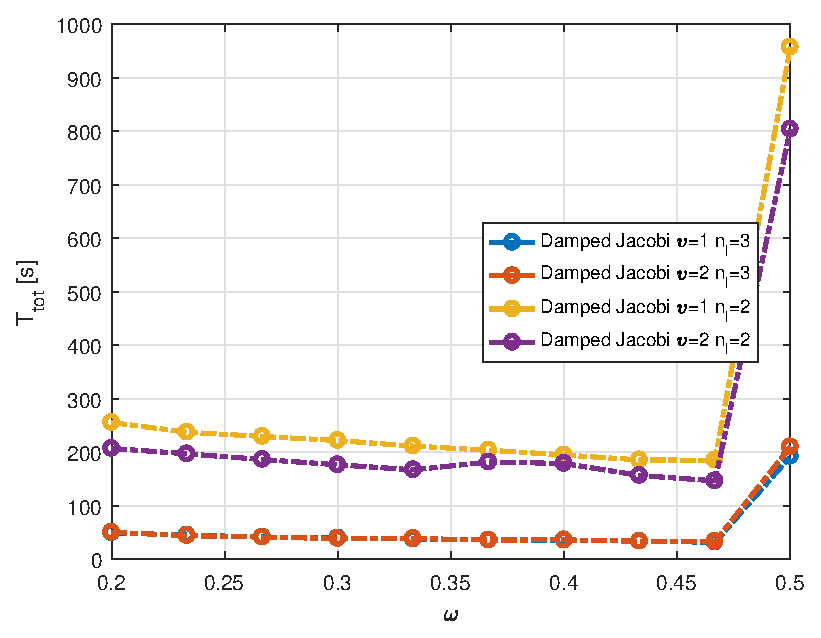
\includegraphics[width=0.5\textwidth]{code_matlab/cputime_Damped_Jacobi.eps}
        }\\
        \subfloat[ \label{fig.1.32c}]{%
          \includegraphics[width=0.5\textwidth]{code_matlab/convergence_speed_Damped_Jacobi.eps}
                       }
        \subfloat[  \label{fig.1.32d}]{%
           \includegraphics[width=0.5\textwidth]{code_matlab/ARR_Damped_Jacobi.eps}
                }
        \caption{Damped Jacobi smoother performances as a function of $\omega$ and for different numbers of mesh levels $n_l$, different numbers of sweeping $\upsilon$. (a) Iterations at convergence.(b) CPU time [s]. (c) Convergence speed defined in equation [Hz] \eqref{eq.cs}. (d) Average Residual Reduction per iteration defined in equation \eqref{eq.arr}. }
        \label{f.1.32}
      \end{figure} 
      In figure \ref{f.1.32} the performances of damped Jacobi smoother are computed for several values of $\omega$, mesh levels $n_l$ and different numbers of sweeping $\upsilon$. One can observe that the minimal CPU time $\approx33$ seconds is reached for $n_l=3$, $\upsilon=2$, $\omega\approx0.47$. 
      One can observe that for $\omega=0.5$ and $\upsilon=1$ the desired accuracy for the relative residual was not reached within 100 iterations. 
      The maximal convergence speed was of $0.35 Hz$, that makes the error reduced by 2.7 at each iteration ( c.f. figure \ref{fig.1.32d}).
       \begin{figure}[hbt!]
         \centering
              \subfloat[ \label{fig.1.33a}]{%
                       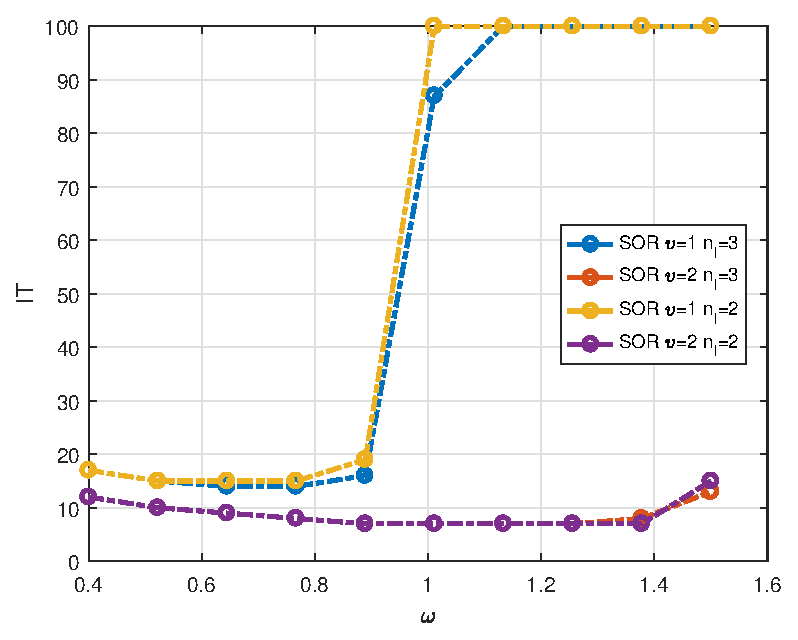
\includegraphics[width=0.5\textwidth]{code_matlab/Iterations_SOR.eps}
                     }
              \subfloat[  \label{fig.1.33b}]{%
                \includegraphics[width=0.5\textwidth]{code_matlab/cputime_SOR.eps}
              }\\
              \subfloat[ \label{fig.1.33c}]{%
                \includegraphics[width=0.5\textwidth]{code_matlab/convergence_speed_SOR.eps}
                             }
              \subfloat[  \label{fig.1.33d}]{%
                 \includegraphics[width=0.5\textwidth]{code_matlab/ARR_SOR.eps}
                      }
              \caption{SOR smoother performances as a function of $\omega$ and for different numbers of mesh levels $n_l$, different numbers of sweeping $\upsilon$. (a) Iterations at convergence.(b) CPU time [s]. (c) Convergence speed defined in equation [Hz] \eqref{eq.cs}. (d) Average Residual Reduction per iteration defined in equation \eqref{eq.arr}.}
              \label{f.1.33}
            \end{figure}
            SOR smoother performances were reported in figure \ref{f.1.33}. In figures \ref{fig.1.33a}  and \ref{fig.1.33b} one can observe a strong dependency of the convergence with the number of sweeping. In fact for $\upsilon=1$ and for $\omega\geq 1$ PCG didn't converged within 100 iterations. The best convergence is obtained for $\omega\approx1.13$, $\upsilon=2$ and $n_l=3$ with 7 iterations in 31 seconds. In figures \ref{fig.1.33c}  and \ref{fig.1.33d} one can also observe that for this point the convergence speed is of $C_S\approx0.4Hz$ and the $ARR\approx6$. This investigation seems to suggest that one could improve performances increasing the number of levels and increasing the number of sweeping. 
            \begin{figure}[hbt!]
                     \centering
                          \subfloat[ \label{fig.1.34a}]{%
                                   \includegraphics[width=0.5\textwidth]{code_matlab/Iterations_Ichol.eps}
                                 }
                          \subfloat[  \label{fig.1.34b}]{%
                            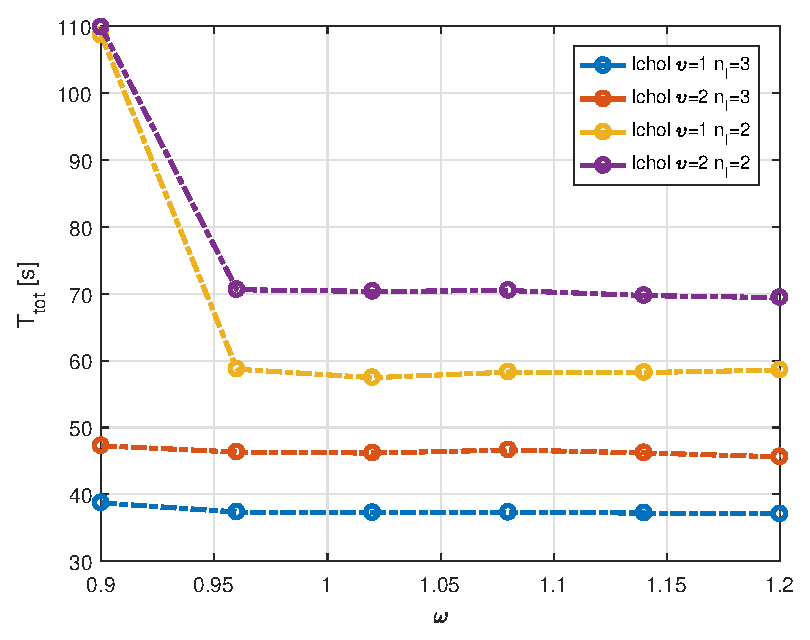
\includegraphics[width=0.5\textwidth]{code_matlab/cputime_Ichol.eps}
                          }\\
                          \subfloat[ \label{fig.1.34c}]{%
                            \includegraphics[width=0.5\textwidth]{code_matlab/convergence_speed_Ichol.eps}
                                         }
                          \subfloat[  \label{fig.1.34d}]{%
                             \includegraphics[width=0.5\textwidth]{code_matlab/ARR_Ichol.eps}
                                  }
                          \caption{Ichol smoother performances as a function of $\omega$ and for different numbers of mesh levels $n_l$, different numbers of sweeping $\upsilon$. (a) Iterations at convergence.(b) CPU time [s]. (c) Convergence speed defined in equation [Hz] \eqref{eq.cs}. (d) Average Residual Reduction per iteration defined in equation \eqref{eq.arr}. }
                          \label{f.1.34}
                        \end{figure}  
                        Ichol smoother performances are described in figure \ref{f.1.34}.  For this method the CPU time include the computation of incomplete Cholesky decompositions for each level. One can observe that much less PCG iterations are needed up to convergence ($\leq 5$). The CPU time per iteration is on the other hand very high and reaches its minimum of 37 seconds for $\omega\approx1.12$ $n_l=3$ and $\upsilon=1$. The maximum convergence speed is reached for the same point $C_S\approx 0.64 Hz$ and is bigger than the value found for the other methods. This means that Ichol smoother has a fast convergence, but still the investment required for the construction of preconditioning is not justified for the accuracy of $10^{-5}$. That is why finally the SOR optimal point is still better than the Ichol point if we look at the total CPU time. If we consider the Line Search variants for Damped Jacobi and Ichol smoother (cf. table \ref{tab:1.1}) we can observe that the fastest combinations are for $\upsilon=1$ and $n_l=3$. The best approach found for this configuration was the LS variant of Ichol with $T_{tot}\approx 37$ seconds. Still this approach is less interesting then Ichol in terms of convergence speed. For a general conclusion based on this configuration, depending on the accuracy needed ichol and LS-ichol smoothers can be effective for applications where strict accuracy is demanded so that the investment on the initial evaluation of the incomplete Cholesky decomposition is repaid by the improved convergence speed. On the other hand SOR and damped Jacobi are very inexpensive and can be adopted in situations where the final accuracy is less critical. Another important criterion of selection that is out of the scope of this work is the scalability of the preconditioner.
                        \begin{table}[h!]
                        % table caption is above the table
                        \caption{Performance of Line Search variants}
                        \label{tab:1.1}       % Give a unique label
                        \centering
                        % For LaTeX tables use
                        \begin{tabular}{lllllll}
                        \hline\noalign{\smallskip}
                        Method & $\upsilon$ & $n_l$ & $IT$ & $T_{tot} [s]$ & $C_S [Hz]$ & $ARR$\\
                        \noalign{\smallskip}\hline\noalign{\smallskip}
                        LS-Damped Jacobi & 1 & 2 & 12 & 53.1 & 0.2348 & 2.78 \\
                        LS-Damped Jacobi & 2 & 2 & 11 & 169.9 & 0.0892 & 2.89 \\
                        LS-Damped Jacobi & 1 & 3 & 18 & 50.5 & 0.2421 & 1.95 \\
                        LS-Damped Jacobi & 2 & 3 & 17 & 208.8 & 0.0699 & 2.01 \\
						LS-Ichol & 1 & 2 & 4 & 52.9 & 0.3384 & 23.1 \\
                        LS-Ichol & 2 & 2 & 4 & 114 & 0.2348 & 39.4 \\
                        LS-Ichol & 1 & 3 & 4 & 37 & 0.5452 & 17.8 \\
                        LS-Ichol & 2 & 3 & 4 & 99.5 & 0.2635 & 23.5 \\
                        \noalign{\smallskip}\hline
                        \end{tabular}
                        \end{table}
\section{Summary and conclusions}      
In this chapter the Finite Element Model approach was reviewed for the resolution of linear elastostatics problems. The optimization framework that is developed in this PhD requires in fact the reliable and fast evaluation of displacements, tip-clearance and stress in a large finite element model including both design space and engine models. In the introduction we also detailed the challenges that this simulation problem represented.  The engine model can be large and complex, to make it available in our Matlab framework, the exploitation of superelements was first reviewed. The design space being meshed in an external environment, 8 node full integration hexahedral elements were reviewed. This gives the freedom to mesh mappable design space geometries that can easily satisfy aerodynamic and integration constraints. The communication between design space mesh and engine model is delicate since discretizations are not consistent at the interface. Several techniques were reviewed and compared with  a new technique we proposed. To make the evaluation of model responses faster in the optimization loop, multigrid preconditioned conjugate gradient was implemented and tested with several smoothers. To summarize the review in this chapter recovered the following topics :
\begin{itemize}
\item Finite Element notation
\item Mesh tying
\item Superelements
\item Multigrid preconditioners
\end{itemize}
A personal contribution was given in:
\begin{itemize}
\item Weighted Average Continuity Approach (WACA) and Moment correction were proposed to deal with mesh tying related issues. Their performances were compared with reviewed approaches on simple 3D examples. Moment correction sensibly improves displacement or stress accuracy of all reviewed technique. Its implementation is recommended in Structural Finite Element models with mesh tying to enforce the local mechanical moment balance at the tied interface. 
\item This work led to the publication of a journal article \cite{coniglio2018weighted}.
\item Different smoother techniques were reviewed and benchmarked on a  demonstration example that includes non-uniform hexahedral elements and the engine superelement for a 3 right hand side vectors application.
\end{itemize}
The studies conducted in this chapter show that our framework, using a combination of reviewed techniques and proposed approaches, provides accurate and relatively fast responses that can be considered consistent with modeling hypothesis.
As possible axes of improvement we can cite:
\begin{itemize}
\item Distributed memory implementations of the provided framework could also be considered as a valid improvement axis. 
\item Other important issue like shear locking control could be introduced in order to improve finite element accuracy.
\item  Still, the major limitation of the proposed framework consists in the fact that the WEM needs to be a linear model to be imported as a superelement. A possible solution in case of nonlinear engine models could be provided by non-intrusive coupling techniques \cite{Gendre2009}.
\end{itemize}
%%% Local Variables: 
%%% mode: latex
%%% TeX-master: "../phdthesis"
%%% End:
